% Options for packages loaded elsewhere
\PassOptionsToPackage{unicode}{hyperref}
\PassOptionsToPackage{hyphens}{url}
%
\documentclass[
  12pt,
  a4paper,
]{report}
\usepackage{lmodern}
\usepackage{setspace}
\usepackage{amssymb,amsmath}
\usepackage{ifxetex,ifluatex}
\ifnum 0\ifxetex 1\fi\ifluatex 1\fi=0 % if pdftex
  \usepackage[T1]{fontenc}
  \usepackage[utf8]{inputenc}
  \usepackage{textcomp} % provide euro and other symbols
\else % if luatex or xetex
  \usepackage{unicode-math}
  \defaultfontfeatures{Scale=MatchLowercase}
  \defaultfontfeatures[\rmfamily]{Ligatures=TeX,Scale=1}
\fi
% Use upquote if available, for straight quotes in verbatim environments
\IfFileExists{upquote.sty}{\usepackage{upquote}}{}
\IfFileExists{microtype.sty}{% use microtype if available
  \usepackage[]{microtype}
  \UseMicrotypeSet[protrusion]{basicmath} % disable protrusion for tt fonts
}{}
\usepackage{xcolor}
\IfFileExists{xurl.sty}{\usepackage{xurl}}{} % add URL line breaks if available
\IfFileExists{bookmark.sty}{\usepackage{bookmark}}{\usepackage{hyperref}}
\hypersetup{
  hidelinks,
  pdfcreator={LaTeX via pandoc}}
\urlstyle{same} % disable monospaced font for URLs
\usepackage[left=2.5cm,right=1.5cm,top=2cm,bottom=2cm]{geometry}
\usepackage{color}
\usepackage{fancyvrb}
\newcommand{\VerbBar}{|}
\newcommand{\VERB}{\Verb[commandchars=\\\{\}]}
\DefineVerbatimEnvironment{Highlighting}{Verbatim}{commandchars=\\\{\}}
% Add ',fontsize=\small' for more characters per line
\newenvironment{Shaded}{}{}
\newcommand{\AlertTok}[1]{\textcolor[rgb]{1.00,0.00,0.00}{\textbf{#1}}}
\newcommand{\AnnotationTok}[1]{\textcolor[rgb]{0.38,0.63,0.69}{\textbf{\textit{#1}}}}
\newcommand{\AttributeTok}[1]{\textcolor[rgb]{0.49,0.56,0.16}{#1}}
\newcommand{\BaseNTok}[1]{\textcolor[rgb]{0.25,0.63,0.44}{#1}}
\newcommand{\BuiltInTok}[1]{#1}
\newcommand{\CharTok}[1]{\textcolor[rgb]{0.25,0.44,0.63}{#1}}
\newcommand{\CommentTok}[1]{\textcolor[rgb]{0.38,0.63,0.69}{\textit{#1}}}
\newcommand{\CommentVarTok}[1]{\textcolor[rgb]{0.38,0.63,0.69}{\textbf{\textit{#1}}}}
\newcommand{\ConstantTok}[1]{\textcolor[rgb]{0.53,0.00,0.00}{#1}}
\newcommand{\ControlFlowTok}[1]{\textcolor[rgb]{0.00,0.44,0.13}{\textbf{#1}}}
\newcommand{\DataTypeTok}[1]{\textcolor[rgb]{0.56,0.13,0.00}{#1}}
\newcommand{\DecValTok}[1]{\textcolor[rgb]{0.25,0.63,0.44}{#1}}
\newcommand{\DocumentationTok}[1]{\textcolor[rgb]{0.73,0.13,0.13}{\textit{#1}}}
\newcommand{\ErrorTok}[1]{\textcolor[rgb]{1.00,0.00,0.00}{\textbf{#1}}}
\newcommand{\ExtensionTok}[1]{#1}
\newcommand{\FloatTok}[1]{\textcolor[rgb]{0.25,0.63,0.44}{#1}}
\newcommand{\FunctionTok}[1]{\textcolor[rgb]{0.02,0.16,0.49}{#1}}
\newcommand{\ImportTok}[1]{#1}
\newcommand{\InformationTok}[1]{\textcolor[rgb]{0.38,0.63,0.69}{\textbf{\textit{#1}}}}
\newcommand{\KeywordTok}[1]{\textcolor[rgb]{0.00,0.44,0.13}{\textbf{#1}}}
\newcommand{\NormalTok}[1]{#1}
\newcommand{\OperatorTok}[1]{\textcolor[rgb]{0.40,0.40,0.40}{#1}}
\newcommand{\OtherTok}[1]{\textcolor[rgb]{0.00,0.44,0.13}{#1}}
\newcommand{\PreprocessorTok}[1]{\textcolor[rgb]{0.74,0.48,0.00}{#1}}
\newcommand{\RegionMarkerTok}[1]{#1}
\newcommand{\SpecialCharTok}[1]{\textcolor[rgb]{0.25,0.44,0.63}{#1}}
\newcommand{\SpecialStringTok}[1]{\textcolor[rgb]{0.73,0.40,0.53}{#1}}
\newcommand{\StringTok}[1]{\textcolor[rgb]{0.25,0.44,0.63}{#1}}
\newcommand{\VariableTok}[1]{\textcolor[rgb]{0.10,0.09,0.49}{#1}}
\newcommand{\VerbatimStringTok}[1]{\textcolor[rgb]{0.25,0.44,0.63}{#1}}
\newcommand{\WarningTok}[1]{\textcolor[rgb]{0.38,0.63,0.69}{\textbf{\textit{#1}}}}
\usepackage{longtable,booktabs}
% Correct order of tables after \paragraph or \subparagraph
\usepackage{etoolbox}
\makeatletter
\patchcmd\longtable{\par}{\if@noskipsec\mbox{}\fi\par}{}{}
\makeatother
% Allow footnotes in longtable head/foot
\IfFileExists{footnotehyper.sty}{\usepackage{footnotehyper}}{\usepackage{footnote}}
\makesavenoteenv{longtable}
\setlength{\emergencystretch}{3em} % prevent overfull lines
\providecommand{\tightlist}{%
  \setlength{\itemsep}{0pt}\setlength{\parskip}{0pt}}
\setcounter{secnumdepth}{5}
% Neoversity formatting preamble. Single source of truth: edit preamble_extra.tex.
% ===========================================================================
% Neoversity academic-research thesis — formatting per
% requirements/Шаблон ... .md (technical formatting block).
% Injected into the pandoc-generated preamble via `pandoc -H`.
% A4; margins L2.5/R1.5/T2/B2 cm (set via -V geometry); Times New Roman;
% body 12pt; headings bold 14pt; line spacing 1.5; paragraph indent 1.25 cm;
% page numbers centred in the bottom footer; chapter titles uppercase.
% ===========================================================================

% --- Fonts: Times New Roman equivalent for pdfLaTeX (portable, no system font) ---
\usepackage{newtxtext}
\usepackage{newtxmath}

% --- Language ---
\usepackage[english]{babel}

% --- Paragraph indent (1.25 cm) instead of inter-paragraph skip ---
\setlength{\parindent}{1.25cm}
\setlength{\parskip}{0pt}

% --- Justified body text is the LaTeX default; keep it. ---

% --- Custom float families: Graph and Chart (separate from Table/Figure) ---
\usepackage{newfloat}
\DeclareFloatingEnvironment[fileext=logrp, listname={List of Graphs}, name=Graph, placement=htbp]{graph}
\DeclareFloatingEnvironment[fileext=lochr, listname={List of Charts}, name=Chart, placement=htbp]{chart}

% --- Number every float family X.Y by chapter ---
\counterwithin{table}{chapter}
\counterwithin{figure}{chapter}
\counterwithin{graph}{chapter}
\counterwithin{chart}{chapter}

% --- Graphics: reference reproducible artifacts under repo root ---
\usepackage{graphicx}
% figures/ holds packaged copies (self-contained, Overleaf-ready); ../../ is the
% in-repo fallback if you build before running the figure-packaging step.
\graphicspath{{figures/}{../../}}

% --- Heading format (titlesec) ---
\usepackage{titlesec}
% Chapter title: bold 14pt, UPPERCASE, centred; 2 blank lines before body text.
\titleformat{\chapter}[hang]
  {\normalfont\bfseries\fontsize{14}{17}\selectfont\filcenter}
  {\MakeUppercase{\chaptertitlename}\ \thechapter.}{1ex}
  {\MakeUppercase}
\titlespacing*{\chapter}{0pt}{0pt}{2\baselineskip}
% Sections / subsections: bold 12pt, left, 1 blank line before body text.
\titleformat{\section}
  {\normalfont\bfseries\fontsize{12}{15}\selectfont}{\thesection}{0.75em}{}
\titlespacing*{\section}{0pt}{1.5\baselineskip}{1\baselineskip}
\titleformat{\subsection}
  {\normalfont\bfseries\fontsize{12}{15}\selectfont}{\thesubsection}{0.75em}{}
\titlespacing*{\subsection}{0pt}{1\baselineskip}{0.5\baselineskip}

% --- Page numbers: centred in the bottom footer on all pages ---
\usepackage{fancyhdr}
\pagestyle{fancy}
\fancyhf{}
\fancyfoot[C]{\thepage}
\renewcommand{\headrulewidth}{0pt}
\renewcommand{\footrulewidth}{0pt}
\fancypagestyle{plain}{%
  \fancyhf{}\fancyfoot[C]{\thepage}%
  \renewcommand{\headrulewidth}{0pt}\renewcommand{\footrulewidth}{0pt}}

% --- Wide data tables: typeset at \small so many-column tables fit A4 width.
%     (Template allows tighter spacing inside tables; line spacing there is 1.) ---
\usepackage{etoolbox}
\AtBeginEnvironment{longtable}{\small}
\usepackage{pdflscape}  % landscape pages for the widest statistics table

% --- Caption style: label and text, small gap ---
\usepackage{caption}
\captionsetup{labelsep=colon, font=normalsize}
\captionsetup[table]{position=top}

% --- \allowbreak breakpoints are injected into long \texttt identifiers/paths
%     by build_thesis.py (post-process), so they wrap inside narrow table
%     columns and never overflow the margin. No hyphen is inserted. ---


\author{}
\date{}

\begin{document}

% Template requires 1.5 line spacing for ALL text (front matter included);
% single spacing only inside tables/figures. Set here so it covers the
% front matter, which is injected before pandoc's own body-level \setstretch.
\setstretch{1.5}

% Front matter (title page, certification, declaration, acknowledgments, TOC,
% the four lists, abbreviations, glossary, abstract). Single source of truth:
% edit frontmatter.tex (it in turn \inputs abbrev/glossary/abstract fragments).
% Fill the remaining <BLANK> fields (dates, signatures) there.
% ===========================================================================
% Front matter (inserted right after \begin{document} via pandoc -B).
% Title page, certification, declaration, acknowledgments, TOC, the four
% lists, abbreviations, glossary, abstract.  Fill the <BLANK> items before
% submission (Student ID, supervisor names, dates, signatures).
% ===========================================================================

% ----------------------------- Title page ---------------------------------
\begin{titlepage}
\thispagestyle{empty}
\centering
\vspace*{2cm}
{\large\bfseries Cross-Modality Validation of Explainable AI Methods for Medical Image Classification: Chest X-ray Pneumothorax and Head CT Hemorrhage Case Studies\par}
\vspace{2cm}
{\normalsize Author: Dmytro Valantsevych\par}
\vspace{1.5cm}
{\normalsize A Master's Thesis submitted to Neoversity in partial fulfillment of the requirements for the degree of Master of Science in Computer Science\par}
\vspace{1cm}
{\normalsize June, 2026\par}
\vspace{2cm}
\begin{flushleft}
Student ID: \underline{1262048355}\\[0.6em]
Thesis Supervisor: \underline{prof. Oleksii Kudin}\\[0.6em]
Co-Supervisor (if applicable): \rule{5cm}{0.4pt}\\[0.6em]
Date of Submission: \rule{4cm}{0.4pt} (target draft cutoff 04/06/2026; defense 21/06/2026)
\end{flushleft}
\vfill
{\footnotesize\itshape \copyright{} The dissertation of Dmytro Valantsevych is approved, and it is acceptable in quality and form for publication electronically.\par}
\end{titlepage}
\setcounter{page}{2}% title page is page 1 (unprinted); avoid duplicate page.1 hyperref destination

% --------------------------- Certification ---------------------------------
\chapter*{Thesis Certification}
\addcontentsline{toc}{chapter}{Thesis Certification}
I confirm that I have reviewed this study and, in my judgment, it adheres to the appropriate standards of academic presentation. I believe it satisfactorily meets the criteria, in terms of both quality and breadth, to serve as a thesis for the attainment of the Master of Science in Computer Science degree. This thesis has been submitted to Neoversity and is deemed sufficient to fulfill the prerequisites for the Master of Science in Computer Science degree.

\vspace{2cm}
\noindent\rule{7cm}{0.4pt}\\
Supervisor

\vspace{1.5cm}
\noindent\rule{7cm}{0.4pt}\\
Co-Supervisor (if applicable)

% ---------------------------- Declaration ----------------------------------
\chapter*{Declaration of Academic Integrity}
\addcontentsline{toc}{chapter}{Declaration of Academic Integrity}
I confirm that this thesis, submitted to fulfill the requirements for the Master of Science in Computer Science degree, completed by me from \underline{13.05.2026} to \rule{3cm}{0.4pt}, is the result of my own individual endeavor. Any contributions from external sources or individuals, including the use of AI tools, are appropriately acknowledged through citation. Furthermore, I confirm that this material has not been previously submitted, in its entirety or in part, for the completion of a degree at this institution or any other.

By making this declaration, I acknowledge that any violation of this statement constitutes academic misconduct. I understand that such misconduct may lead to expulsion from the program and/or disqualification from receiving the degree.

\vspace{0.8cm}
\noindent Name of the Candidate: Dmytro Valantsevych

\vspace{1.2cm}
\noindent Signature of Candidate: \rule{6cm}{0.4pt}\hfill Date: \rule{3.5cm}{0.4pt}


% -------------------------- Acknowledgments --------------------------------
\chapter*{Acknowledgments}
\addcontentsline{toc}{chapter}{Acknowledgments}
I would like to express my sincere gratitude to my thesis supervisor, prof.~Oleksii Kudin, for his guidance, constructive feedback, and support throughout the planning and execution of this research. I am also grateful to the faculty of Neoversity for the academic foundation on which this work builds, prof.~Kateryna Doikova, prof.~Dmytro Doikov, Dmitry Balabka MCSc, Kateryna Strembitska MD for support throughout planning of this research, and to my family and friends for their patience and encouragement during the intense period of experiments and writing.

\vspace{0.8cm}
\noindent\textbf{Use of artificial intelligence tools.} In the interest of transparency and in accordance with the academic integrity requirements of this program, the author discloses the following use of AI and AI-assisted development tools during the research workflow:

\begin{itemize}
  \item \textbf{GPT-5.5 and Codex} (OpenAI, \url{https://openai.com/}) were used for code assistance (writing, refactoring, and debugging of experiment code) and for brainstorming and planning discussions around experiment design.
  \item \textbf{Claude Sonnet~4.6, Claude Opus~4.7, and Claude Opus~4.8} (Anthropic, \url{https://www.anthropic.com/claude}), operated through the Claude Code (\url{https://claude.com/claude-code}) and \textbf{Junie} (\url{https://www.jetbrains.com/junie/}) agentic environments, were used for pipeline code development, experiment automation, drafting of research documentation and thesis draft text, and the \LaTeX{} build of this document.
  \item \textbf{PyCharm} with the \textbf{Junie} assistant (JetBrains, \url{https://www.jetbrains.com/pycharm/}, \url{https://www.jetbrains.com/junie/}) and \textbf{VS~Code} (Microsoft, \url{https://code.visualstudio.com/}) served as development environments with integrated AI coding assistance from the above-mentioned models for the experiment pipeline.
\end{itemize}

\noindent\textbf{Oversight and responsibility.} All AI-assisted output -- code and text alike -- was reviewed, tested, and verified by the author, who directed every stage of the work and bears full responsibility for the content of this thesis. No AI tool is an author of this work. All experimental results reported in Chapter~4 were produced by the author's locally executed analysis pipeline, not generated by an AI tool.

\vspace{0.4cm}
\noindent\textbf{Data handling.} Only source code and draft text were processed with AI tools. All datasets and dataset-related information (medical images, annotation masks, and derived per-case data) were processed exclusively by locally executed code and were never submitted to any AI tool or external service.

% --------------------- Contents and the four lists -------------------------
\tableofcontents
\listoftables
\listoffigures
\listofgraphs
\listofcharts

% ----------------------- List of Abbreviations -----------------------------
\chapter*{List of Abbreviations}
\addcontentsline{toc}{chapter}{List of Abbreviations}
\begin{longtable}{@{}l p{0.72\linewidth}@{}}
\toprule
\textbf{Abbreviation} & \textbf{Full Form}\\
\midrule
\endhead
ACM & Association for Computing Machinery\\
AI & Artificial Intelligence\\
CLAIM & Checklist for Artificial Intelligence in Medical Imaging\\
CNN & Convolutional Neural Network\\
CT & Computed Tomography\\
CVF & Computer Vision Foundation\\
CXR & Chest X-ray\\
DECIDE-AI & Developmental and Exploratory Clinical Investigations of Decision support systems driven by Artificial Intelligence\\
DL & Deep Learning\\
FN & False Negative\\
FP & False Positive\\
Grad-CAM & Gradient-weighted Class Activation Mapping\\
HU & Hounsfield Unit\\
IEEE & Institute of Electrical and Electronics Engineers\\
IHD & Intracranial Hemorrhage Detection\\
IG & Integrated Gradients\\
IoU & Intersection over Union\\
ML & Machine Learning\\
NeurIPS & Conference on Neural Information Processing Systems\\
P@F & Precision at Fraction (precision of the selected top-fraction attribution pixels)\\
PMLR & Proceedings of Machine Learning Research\\
ROC-AUC & Area Under the Receiver Operating Characteristic Curve\\
SHAP & SHapley Additive exPlanations\\
SIIM-ACR & Society for Imaging Informatics in Medicine - American College of Radiology\\
TN & True Negative\\
TP & True Positive\\
XAI & Explainable Artificial Intelligence\\
\bottomrule
\end{longtable}


% --------------------------- Glossary --------------------------------------
\chapter*{Glossary of Methodological Terms}
\addcontentsline{toc}{chapter}{Glossary of Methodological Terms}
\textbf{Attribution map / heatmap} - A two-dimensional visualization
derived from a trained classifier that assigns relative importance to
image regions for a selected output score. In this thesis, attribution
maps are class-specific evidence maps for the selected pneumothorax or
hemorrhage target, not automatic anatomical segmentations.

\textbf{Positive evidence} - The part of a signed attribution map that
contributes positively toward the selected target output. For the CXR
pneumothorax experiments, positive evidence supports the model's
pneumothorax score.

\textbf{Negative evidence} - The part of a signed attribution map that
contributes negatively toward the selected target output. Negative
evidence is interpreted as suppressive evidence against the target score
and is considered significant for potential improvement when it overlaps 
the lesion mask.

\textbf{Magnitude view} - The absolute-value view of a signed
attribution map. It answers which pixels were influential, without
stating whether their influence increased or decreased the target score.

\textbf{Signed view} - A diverging visualization of the normalized
signed attribution map. It summarizes the local balance between positive
and negative evidence but does not replace inspection of the separate
positive, negative, and magnitude views.

\textbf{Selected view} - A visualization of other views using their absolute values and disregarding the alpha value.

\textbf{Localization validation} - Evaluation of whether
high-attribution pixels spatially correspond to available lesion
annotations, using metrics such as IoU, Dice, pointing-hit, and
precision-at-fraction.

\textbf{Faithfulness validation} - Evaluation of whether the highlighted
pixels materially affect the model's own output probability when they
are removed, replaced, or inserted. Faithfulness measures model
behavior, not clinical correctness.

\textbf{Top-fraction thresholding} - Conversion of a continuous heatmap
into a binary selected region by keeping a fixed fraction of the
highest-valued pixels. This makes heatmaps comparable to masks but
introduces a threshold choice that must be calibrated or reported.

\textbf{Coverage saturation} - A secondary diagnostic describing how
quickly top-fraction thresholding expands to cover nearly the whole
image. The proposed \texttt{coverage\_saturation\_fraction\_95} records
the smallest swept top-fraction at which selected coverage reaches at
least \texttt{95\%}; lower values indicate more diffuse or saturated
maps.

\textbf{Radiologist-centered review} - A structured qualitative
assessment in which a medically trained reader scores explanation
localization, usefulness, and failure mode categories under a fixed
review task. In this thesis it is an early controlled assessment, not
prospective clinical validation.


% ---------------------------- Abstract -------------------------------------
\chapter*{Abstract}
\addcontentsline{toc}{chapter}{Abstract}
This work investigates how explainable artificial intelligence methods
can be applied for medical image classification rather than used only as
visual illustrations. The study focuses primarily on chest X-ray
pneumothorax detection using the SIIM-ACR pneumothorax dataset and
off-the-shelf TorchXRayVision classifiers, with a completed head CT
intracranial hemorrhage pilot used as a cross-modality methodological
extension. The aim is to compare several post-hoc explanation methods
against out-of-the-box medical classification models and assess whether
their highlighted evidence is localized, faithful to the model, and
clinically useful.

The methodology separates classifier behavior from explanation quality.
Pneumothorax classifiers are evaluated at frozen thresholds, while
explanation maps are generated with CAM-family, SHAP and Occlusion
methods, and a frozen four-method consensus. Each method is interpreted
through positive, negative, magnitude, and signed views. Explanations
are validated with lesion-mask localization metrics, negative-evidence
diagnostics, deletion/insertion faithfulness curves, method-agreement
analysis, and a structured radiologist-style review of selected cases.

Current CXR results show that DenseNet-chex supersedes the original
DenseNet-all checkpoint as the selected DenseNet baseline, while
ResNet-50 remains the strongest tested TorchXRayVision follow-up in
relative localization terms; nevertheless, absolute pneumothorax-mask
overlap remains weak. The held-out Phase 5.2 improvement experiment
shows model-dependent consensus behavior: DenseNet-chex consensus mainly
improves over Score-CAM in paired overlap tests, whereas ResNet-50
consensus significantly improves Dice/IoU over several weaker individual
methods but not over the strongest CAM comparators. The balanced 40-case
review shows mixed usefulness: many maps contain interpretable evidence,
yet clinically misleading, indirect, device-related, or high-contrast
non-lesion evidence remains common.

The practical significance of the work is a reproducible validation
workflow for auditing medical image explanations. The thesis argues that
heatmaps should be treated as model-behavior diagnostics, not anatomical
segmentations or automatic generators of clinical trust.

Keywords: explainable artificial intelligence, medical image
classification, radiology, Grad-CAM, SHAP, pneumothorax, intracranial
hemorrhage


\cleardoublepage


% Body chapters (1-5) + appendices. Single source of truth: edit body.tex.
\hypertarget{introduction}{%
	\chapter{Introduction}\label{introduction}}

\hypertarget{research-context}{%
	\section{Research Context}\label{research-context}}

Deep learning has become a central technology in medical image analysis
because convolutional and transformer-based models can learn
discriminative image patterns from large radiology datasets
\cite{ref-medical-xai-review}. In chest radiography and computed
tomography, such models can support classification tasks such as
pneumothorax detection or intracranial hemorrhage screening. However,
the clinical usefulness of a model cannot be judged only from an
image-level prediction score. In high-risk medical settings, a
prediction is acceptable only when the evidence behind it can
be inspected and compared with expected clinical findings.

Explainable AI (XAI) methods are often proposed as a way to make deep
learning systems more transparent. Saliency, class activation,
occlusion, and attribution maps can highlight image regions that
contribute to a model output. These visualizations are especially
attractive in radiology because they resemble the spatial reasoning used
by a radiologist. Nevertheless, a visually plausible heatmap is not
automatically a clinically valid explanation
\cite{ref-saliency-trust-medical}. A model may highlight devices, image
borders, text markers, bone edges, or treatment-related correlates
rather than the visible pathology itself \cite{ref-clever-hans}.

This thesis addresses the gap between visual and
clinically relevant explanation. It treats XAI maps as class-specific
model-behavior diagnostics, not as direct pathology segmentations. The
primary empirical setting is chest X-ray pneumothorax classification on
the SIIM-ACR pneumothorax dataset using off-the-shelf TorchXRayVision
classifiers. A completed head CT hemorrhage pilot against a PhysioNet masked
CT dataset and a DifeiT Vision Transformer classifier was included as a
methodological extension after verifying the transferability of the designed approach.
The CT branch is intentionally narrower than the CXR study and is used to test whether
the validation workflow transfers across modality.

\hypertarget{problem-statement-and-relevance}{%
	\section{Problem Statement and
		Relevance}\label{problem-statement-and-relevance}}

Medical image classifiers can achieve high metric scores 
while relying on features that are not aligned
with the target abnormality at all. This creates a validation
problem: if the explanation map is interpreted as evidence that the
model ``looked at the right place'', the explanation itself is considered
as an argument to trust this model. However, without proper validation, 
the explanation may be clinically misleading.

The problem addressed here is therefore the clinical and
methodological reliability of post-hoc XAI explanations for medical
image classification. The key questions in this thesis are whether
the mask localizes to available lesion evidence,
whether it faithfully affects the model output under perturbation,
whether different XAI methods agree, and whether a
medically trained reviewer judges the explanation useful or misleading.

The thesis is guided by the following research questions:

\begin{enumerate}
	\def\labelenumi{\arabic{enumi}.}
	\tightlist
	\item
	Do off-the-shelf medical image classifiers produce clinically
	localized explanations on SIIM-ACR pneumothorax cases?
	\item
	How do common XAI methods differ when evaluated by mask-overlap
	metrics, peak-localization metrics, faithfulness curves, and
	signed-evidence diagnostics?
	\item
	Does a frozen cross-method consensus improve localization compared
	with individual methods under held-out paired testing?
	\item
	Can structured radiologist-style review reveal explanation failure
	modes that are not captured by automatic metrics alone?
	\item
	To what extent does the same validation design transfer to a second
	modality such as head CT hemorrhage without over-claiming empirical
	cross-modality results?
\end{enumerate}

\hypertarget{aim-and-research-objectives}{%
	\section{Aim and Research
		Objectives}\label{aim-and-research-objectives}}

Aim: To compare, validate, and clinically assess explainable AI methods
for medical image classification across chest X-ray pneumothorax and
head CT hemorrhage case studies.

Objectives:
\begin{itemize}
\item Review recent literature on XAI methods in radiology.
\item Reuse classification models for pneumothorax and intracranial
hemorrhage detection.
\item Generate explanation maps using multiple XAI methods.
\item Validate explanations against lesion masks using quantitative
localization metrics.
\item Perform radiologist-centered qualitative assessment of explanation
usefulness and failure modes.
\item Test a simple improvement strategy for explanation maps.
\end{itemize}

\hypertarget{scientific-novelty-and-practical-significance}{%
	\section{Scientific Novelty and Practical
		Significance}\label{scientific-novelty-and-practical-significance}}

The scientific novelty of the work lies in viewing XAI heatmaps and techniques
as a complex practical question of model trust instead of simple illustration. 
The thesis combines classifier-threshold calibration,
lesion-mask localization metrics, perturbation-based faithfulness
curves, signed positive/negative evidence views, method agreement
analysis, and radiologist-centered failure taxonomy within one
reproducible pipeline. This design makes it possible to distinguish four
ideas that are often conflated: a correct classifier prediction, a
lesion-overlapping explanation, a model-faithful explanation, and a
clinically useful explanation.

The work also contributes a cautionary empirical case study. The
baseline models are not fine-tuned, but intentionally selected 
off-the-shelf medical image classifiers. This is practically
important because pretrained clinical AI tools are often reused outside
their exact development distribution. Showing that a pretrained model
can be moderately predictive while producing weakly localized or
confounded explanations demonstrates why explanation validation 
is necessary before heatmaps are used to support model trustworthiness.

The practical significance of this work is also a validation workflow that
can be used to audit medical image explanations. The same workflow can support
new model comparison, including pneumothorax-specific, larger
radiologist studies, and expansions over new diagnostic modalities. 
In clinical terms, the intended contribution is a safe
interpretation of model evidence, specifically use of XAI maps 
to identify when the model output and its explanation should not be trusted.

\hypertarget{thesis-structure}{%
	\section{Thesis Structure}\label{thesis-structure}}

Chapter 1 presents the research context, states the problem, aim,
objectives, and contribution. Chapter 2 reviews available literature
with known usages of deep learning models in radiology, post-hoc XAI methods, explanation-validation approaches, and 
known risks such as shortcut learning and visually plausible but
unreliable saliency maps. Chapter 3 describes the experimental
methodology, including datasets, preprocessing, classifier baselines,
XAI methods, threshold calibration, localization and faithfulness
metrics, statistical testing, and radiologist-centered review. Chapter 4
presents and discusses the empirical results, including classifier
behavior, quantitative explanation validation, model comparison,
radiologist review, CXR consensus-improvement experiments, and the
completed CT experiment. Chapter 5 provides the general conclusion, summarizing 
the main findings, practical recommendations, limitations, and thoughts on future work.

\hypertarget{conclusions-to-chapter-1}{%
	\section*{Conclusions to Chapter 1}\label{conclusions-to-chapter-1}}
\addcontentsline{toc}{section}{Conclusions to Chapter 1}

In Chapter 1, the focus was to define the scope, pose the research problem,
identify objectives and goals, as well as provide pre-research questions
and hypotheses. Deep learning models can produce useful predictions in
radiology, but the clinical meaning of those predictions (and especially 
their reliability) depends on the image evidence used by the model. 
Post-hoc heatmaps can make this evidence visible, 
however, the information itself has to be correctly interpreted. The heatmap
may emphasize non-pathological structures, and as such will not
help data scientists understand the root cause of insufficient performance.
The claim of this work is that explanation maps should not be considered 
as an anatomic segmentation or considered in isolation from the model itself 
and the dataset. 

The research problem is the reliability of XAI explanations for medical
image classification and the goal is to expose this confusion and contribute
to reliable and reproducible usage of AI in radiology.

\hypertarget{literature-review}{%
	\chapter{Literature Review}\label{literature-review}}

\hypertarget{literature-search-strategy}{%
	\section{Literature Search Strategy}\label{literature-search-strategy}}

The literature review uses peer-reviewed papers, official dataset and model
documentation, and guidance on medical-imaging AI reporting. The source selection categories were: (1) deep learning for radiology and public chest
X-ray datasets; (2) post-hoc XAI methods for image classifiers; (3)
explanation-validation methods, including localization,
perturbation-based faithfulness, sanity checks, and human-centered
evaluation; (4) shortcut learning and clinical applicability risks; and
(5) transparent reporting and risk-of-bias guidance for medical AI
studies.

The review sources include official proceedings pages,
journal records, PubMed entries,
CVF, PMLR, NeurIPS, IEEE, ACM records, official dataset pages, and
software documentation. Blogs, informal tutorials, and unverified
dataset mirrors are excluded unless explicitly justified. Online sources
include stable URLs and access dates, and the bibliography follows the
IEEE style consistently.

The review emphasizes recent literature from approximately 2016 onward
because most widely used post-hoc deep-learning XAI methods and
medical-imaging AI reporting frameworks emerged or matured during this
period. Older sources are retained where historically necessary, such as
occlusion sensitivity and early convolutional-network visualization
work.

\hypertarget{deep-learning-classification-in-radiology}{%
	\section{Deep Learning Classification in
		Radiology}\label{deep-learning-classification-in-radiology}}

Deep learning classifiers have become common in radiology research
because they can learn hierarchical image features directly from pixel
data. Chest X-ray is a particularly active domain: it is widely
available, clinically important, and represented in large public
datasets such as ChestX-ray14 \cite{ref-chestxray8}, CheXpert
\cite{ref-chexpert}, MIMIC-CXR \cite{ref-mimic-cxr}, and VinDr-CXR \cite{ref-vindr-cxr}.
These datasets enabled the creation of
pretrained CXR models, radiologist-comparison classifiers
\cite{ref-chexnext}, and libraries, including TorchXRayVision
\cite{ref-torchxrayvision}, which provide practical baselines for
downstream research.

However, public CXR datasets are not interchangeable. They differ in
institutions, acquisition workflows, label extraction quality,
uncertainty handling, disease prevalence, and availability of
localization annotations. Many labels are derived from radiology reports
rather than pixel-level lesion masks. As a result, a classifier can
learn image-level associations that support prediction without
necessarily learning spatial evidence that aligns with a lesion
annotation. This distinction is key to this thesis:
image-level classifier performance and explanation localization must be
reported separately.

Pneumothorax is a useful focused case study because it has high
clinical relevance and segmentation masks are available from the SIIM-ACR challenge
\cite{ref-siim-acr}.
These masks make it possible to evaluate whether model explanations
overlap the visible abnormality. The thesis uses strictly off-the-shelf
models as baselines rather than locally fine-tuned
pneumothorax segmenters, and TorchXRayVision was selected as the easiest to use for
this purpose. This study investigates how pretrained medical
classifiers behave when their explanations are tested against a specific
pneumothorax localization reference.

Head CT intracranial hemorrhage \cite{ref-rsna-ihd} is methodologically
relevant as a second modality because it differs from radiography in
image physics, intensity scale, preprocessing, and clinically meaningful
perturbation baselines. CT data are typically represented in Hounsfield
units and interpreted through diagnostic windows, whereas CXR inputs are
2D radiographs with different normalization assumptions. In this study,
CT coverage was limited, and the purpose was to validate cross-modality
transferability with one verified pretrained classifier and one public
masked dataset.

\hypertarget{explainable-ai-methods-for-image-classification}{%
	\section{Explainable AI Methods for Image
		Classification}\label{explainable-ai-methods-for-image-classification}}

Post-hoc XAI methods for image classifiers can be grouped by the type of
signal they use \cite{ref-medical-xai-review}. CAM-family methods use
internal convolutional feature maps to produce class-discriminative
spatial maps. For instance, Grad-CAM \cite{ref-gradcam} applies weights to
target-layer activations based on gradients of the selected class score, while
Grad-CAM++ \cite{ref-gradcampp} uses a modified gradient-weighting
scheme to better handle multiple or fine-grained discriminative regions.
These methods are attractive for radiological tasks because they produce
relatively smooth, spatially coherent maps, but their resolution and
interpretation are limited by the selected feature layer.

Eigen-CAM \cite{ref-eigen-cam} and Score-CAM
\cite{ref-scorecam} extend the CAM family in different directions.
Eigen-CAM derives a map from the principal component of
target-layer activations and does not require gradients, while
Score-CAM masks the input with normalized activation maps and
weights them according to score changes. In this work, both
are included as individual methods, both for comparison and as part of selecting the most suitable CAM-family
method.

Pixel-attribution methods answer a different question. 
Integrated Gradients \cite{ref-integrated-gradients}
accumulates gradients along each path from a baseline image to the input,
making baseline choice an explicit part of the explanation.
GradientSHAP approximates Shapley-style attributions
\cite{ref-shap} through noisy baseline interpolation and is therefore
stochastic. 
In medical images, these methods can reveal fine-grained evidence extracted at the
pixel level, but the quality of such evidence may be affected by noise, intermediate gradients,
and non-specificity of the model itself, as in multi-class classifiers, where
the model is expected to mark general areas. The baseline also affects
quality, so it has to be selected carefully and should be a truly classifier-neutral
source.

Perturbation methods evaluate model behavior under direct image
modification. Occlusion \cite{ref-occlusion-zeiler} replaces
patches of the image and measures how the selected class score changes.
This makes it conceptually close to faithfulness testing because it asks
what happens to the classifier when regions are removed or replaced.
However, Occlusion is computationally expensive and sensitive to patch
size, stride, and replacement baseline. In this work, it is treated
as a complementary diagnostic tool rather than as a direct
substitute for gradient attribution.

\texttt{LIME} \cite{ref-lime} represents a region-level surrogate-model
family: it perturbs interpretable image regions and fits a local linear
approximation to the classifier. In this thesis it is not implemented
and is referenced only as a direction for future research.
Its conceptual value is that it belongs to a different
explanation family and introduces segmentation with perturbation.

The implemented CXR methods share a \texttt{Signed Attribution} contract.
Each method can provide positive evidence, negative evidence, magnitude,
and signed views. This is important for a radiologist because these views
answer different interpretive questions. A
positive-evidence map should not be scored as clinically successful
merely because it overlaps a lesion mask.

Table \ref{table:2-1} summarizes how the main XAI method families differ and why
none of them is sufficient as a standalone validation signal.

\begin{longtable}[]{@{}llll@{}}
	\caption{Summary of XAI method families and validation
		concerns}\tabularnewline
	\toprule
	\begin{minipage}[b]{0.22\columnwidth}\raggedright
		Method family\strut
	\end{minipage} & \begin{minipage}[b]{0.22\columnwidth}\raggedright
		Examples in thesis\strut
	\end{minipage} & \begin{minipage}[b]{0.22\columnwidth}\raggedright
		Main question answered\strut
	\end{minipage} & \begin{minipage}[b]{0.22\columnwidth}\raggedright
		Main validation concern\strut
	\end{minipage}\tabularnewline
	\midrule
	\endfirsthead
	\toprule
	\begin{minipage}[b]{0.22\columnwidth}\raggedright
		Method family\strut
	\end{minipage} & \begin{minipage}[b]{0.22\columnwidth}\raggedright
		Examples in thesis\strut
	\end{minipage} & \begin{minipage}[b]{0.22\columnwidth}\raggedright
		Main question answered\strut
	\end{minipage} & \begin{minipage}[b]{0.22\columnwidth}\raggedright
		Main validation concern\strut
	\end{minipage}\tabularnewline
	\midrule
	\endhead
	\begin{minipage}[t]{0.22\columnwidth}\raggedright
		CAM-family activation maps\strut
	\end{minipage} & \begin{minipage}[t]{0.22\columnwidth}\raggedright
		Grad-CAM, Grad-CAM++, Eigen-CAM,
		Score-CAM\strut
	\end{minipage} & \begin{minipage}[t]{0.22\columnwidth}\raggedright
		Which target-layer activation regions support the selected class
		score?\strut
	\end{minipage} & \begin{minipage}[t]{0.22\columnwidth}\raggedright
		Spatial resolution, target-layer choice, and possible focus on
		discriminative but non-lesion regions
		
		\strut
	\end{minipage}\tabularnewline
	\begin{minipage}[t]{0.22\columnwidth}\raggedright
		Pixel attribution\strut
	\end{minipage} & \begin{minipage}[t]{0.22\columnwidth}\raggedright
		Integrated Gradients, GradientSHAP\strut
	\end{minipage} & \begin{minipage}[t]{0.22\columnwidth}\raggedright
		Which input pixels contribute positively or negatively relative to a
		baseline?\strut
	\end{minipage} & \begin{minipage}[t]{0.22\columnwidth}\raggedright
		Baseline sensitivity, stochasticity, pixel noise, smoothing, and
		case-invariant patterns\strut
	\end{minipage}\tabularnewline
	\begin{minipage}[t]{0.22\columnwidth}\raggedright
		Perturbation sensitivity\strut
	\end{minipage} & \begin{minipage}[t]{0.22\columnwidth}\raggedright
		Occlusion\strut
	\end{minipage} & \begin{minipage}[t]{0.22\columnwidth}\raggedright
		How does the model score change when image patches are replaced?\strut
	\end{minipage} & \begin{minipage}[t]{0.22\columnwidth}\raggedright
		Patch size, stride, replacement baseline, and computational cost\strut
	\end{minipage}\tabularnewline
	\begin{minipage}[t]{0.22\columnwidth}\raggedright
		Cross-method consensus\strut
	\end{minipage} & \begin{minipage}[t]{0.22\columnwidth}\raggedright
		consensus, signed consensus\strut
	\end{minipage} & \begin{minipage}[t]{0.22\columnwidth}\raggedright
		Do several explanation families agree on spatial evidence?\strut
	\end{minipage} & \begin{minipage}[t]{0.22\columnwidth}\raggedright
		Taking an average from weak or mislocalized maps may not create 
		clinically aligned evidence\strut
	\end{minipage}\tabularnewline
	\begin{minipage}[t]{0.22\columnwidth}\raggedright
		Region-level surrogate methods\strut
	\end{minipage} & \begin{minipage}[t]{0.22\columnwidth}\raggedright
		\texttt{LIME}\strut
	\end{minipage} & \begin{minipage}[t]{0.22\columnwidth}\raggedright
		Which interpretable regions support a local surrogate
		approximation?\strut
	\end{minipage} & \begin{minipage}[t]{0.22\columnwidth}\raggedright
		Superpixel definition, perturbation distribution, local-model stability,
		and separate calibration needs\strut
	\end{minipage}\tabularnewline
	\bottomrule
	\label{table:2-1}
\end{longtable}

\hypertarget{validation-of-explanations}{%
	\section{Validation of Explanations}\label{validation-of-explanations}}

Explanation validation has several non-equivalent dimensions.
Localization validation compares selected attribution regions with
available reference annotations
\cite{ref-chexlocalize, ref-cxr-saliency-benchmark}. In this thesis the
main positive-localization metrics are \texttt{IoU}, \texttt{Dice},
\texttt{pointing \allowbreak hit}, and \texttt{P@F}.
\texttt{IoU}, \texttt{Dice}, and \texttt{P@F} summarize overlap
between selected heatmap regions and the pneumothorax mask, while
\texttt{pointing \allowbreak hit} is stricter: it checks whether the
maximum-attribution point falls inside the lesion. These metrics are
useful for positive cases with masks, but they do not fully capture
clinical usefulness.

Faithfulness validation asks whether the highlighted pixels materially
influence the model's own output
\cite{ref-samek-evaluation, ref-meaningful-perturbation}. Deletion
curves start from the original image and replace highly attributed
pixels; insertion curves start from a baseline image and restore highly
attributed pixels \cite{ref-rise}. If an explanation is faithful to the
classifier, deleting high-attribution regions should reduce the target
probability relatively quickly, while inserting them should restore it
quickly too. This evaluates model behavior, not clinical correctness. A
heatmap may be faithful to a shortcut-driven model while still failing
to localize the annotated lesion.

Sanity checks \cite{ref-sanity-checks} and robustness analyses
\cite{ref-infidelity-sensitivity} are also important because saliency
methods can sometimes produce visually stable maps even when model
parameters or labels are changed. In medical imaging, this concern is
increased by structured preprocessing, strong anatomical priors, and
recurring acquisition artifacts. For pixel-level methods such as
Integrated Gradients and GradientSHAP, smoothing and cross-case
similarity should be reported so that readers can distinguish
case-specific evidence from generic image patterns.

Human-centered evaluation complements automatic metrics
\cite{ref-human-centered-xai}. A radiologist-style reviewer can identify
whether a map highlights direct lesion evidence, indirect clinically
related evidence, treatment correlates, devices, text artifacts,
non-pathological high-contrast anatomy, or misleading regions. This type
of review should be treated as structured qualitative evidence, not as
prospective clinical validation. Its value is that it exposes clinically
meaningful failure modes that a mask-overlap score may miss.

The central limitation of saliency maps is that they are easy to
over-interpret
\cite{ref-false-hope-xai, ref-radiology-interpretability}. They can show
where attribution is high, but they do not prove causality in the
clinical sense, and they do not replace reporting of the model, data,
target class, preprocessing, perturbation baseline, thresholding rule,
or calibration split. For this reason, the thesis reports explanation
maps together with classifier behavior, localization metrics,
faithfulness curves, and review scores.

\begin{figure}[htbp]
	\centering
	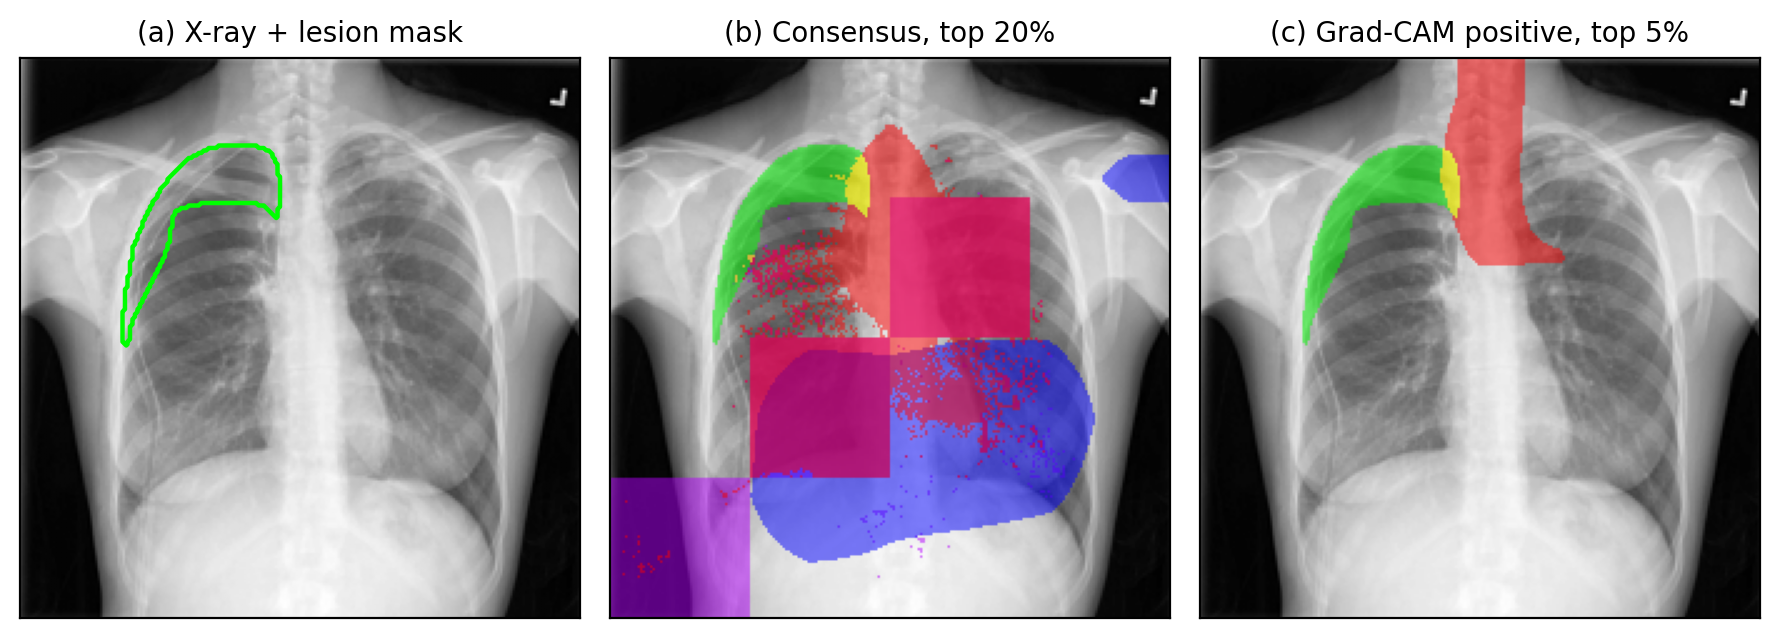
\includegraphics[width=0.95\linewidth,height=0.32\textheight,keepaspectratio]{figures/iter_27_classifier_outcome_any5000_balanced100_all_methods__fn__1065_train_1__figure_2_1_composite.png}
	\caption{Conceptual risk of visually plausible but clinically misleading saliency maps.}
	\label{figure:2-1}
	\smallskip
	\begin{minipage}{0.95\linewidth}
		\footnotesize
		(a) Chest X-ray with the annotated pneumothorax mask (green contour) in the right lung apex. (b) Consensus attribution at the top 20\% selected fraction and (c) Grad-CAM positive evidence at the top 5\% selected fraction concentrate on central, mediastinal regions and largely miss the annotated lesion.
	\end{minipage}
\end{figure}

Figure~\ref{figure:2-1} illustrates that a heatmap can be visually plausible
while highlighting clinically indirect or confounded image regions
rather than the annotated lesion.

\hypertarget{research-gap}{%
	\section{Research Gap}\label{research-gap}}

The reviewed literature supports three conclusions. First, deep learning
classifiers can be useful in radiology, but image-level performance does
not guarantee lesion-aligned reasoning
\cite{ref-cxr-generalization-zech, ref-hidden-stratification}. Second,
XAI methods are diverse and method-dependent: CAM maps, pixel
attributions, Shapley-style approximations, and occlusion diagnostics
answer different questions. Third, explanation validation remains
difficult because a visually plausible heatmap may be unfaithful, poorly
localized, or clinically misleading.

The research gap addressed by this thesis is the lack of a compact but
layered validation workflow that compares several XAI methods on the
same medical imaging task using mask localization, perturbation
faithfulness, method agreement, signed-evidence interpretation, and
radiologist-centered failure review. Many studies present heatmaps as
qualitative illustrations; fewer test whether those heatmaps align with
available lesion masks, whether they affect the model output under
controlled perturbation, and whether a medically trained reviewer finds
them useful or misleading.

The thesis also focuses on a practically important negative possibility:
a pretrained medical classifier may be predictive enough to appear
useful while its explanations reveal shortcut learning
\cite{ref-shortcut-learning, ref-radiology-shortcuts}, weak clinical
localization, or reliance on confounders rather than being right for the
right reasons \cite{ref-right-reasons, ref-race-medical-imaging}.
Demonstrating this failure mode is scientifically valuable because it
clarifies what XAI can and cannot justify. The contribution is not the
claim that heatmaps automatically create trust, but that validated
heatmaps can help decide when trust should be withheld.

\hypertarget{conclusions-to-chapter-2}{%
	\section*{Conclusions to Chapter 2}\label{conclusions-to-chapter-2}}
\addcontentsline{toc}{section}{Conclusions to Chapter 2}

Chapter 2 reviewed the literature background needed for the thesis. Deep
learning classifiers are now common in radiology research, especially in
chest X-ray analysis, but public dataset labels, source institutions,
and clinical contexts differ substantially. A model trained or
pretrained on one data mixture cannot be assumed to localize pathology
correctly on another dataset. This motivates the decision to
evaluate off-the-shelf TorchXRayVision baselines not only by image-level
prediction, but also by explanation localization and qualitative failure
modes.

The reviewed XAI methods form complementary families. CAM-family methods
provide class-discriminative spatial maps from internal activations;
pixel-attribution methods trace gradients or Shapley-style contributions
back to the input; occlusion directly perturbs image regions; and
surrogate approaches such as LIME explain local behavior through
interpretable region perturbations. Because these methods answer
different questions, agreement between them is stronger evidence than
any single heatmap, while disagreement is itself diagnostically useful.

The validation literature shows that heatmaps must be tested rather than
merely displayed. Localization metrics, faithfulness curves, robustness
checks, and human-centered review each capture different aspects of
explanation quality. In medical imaging, this is especially important
because shortcut cues, devices, acquisition artifacts, and
non-pathological high-contrast anatomy can all become model evidence.
The research design in Chapter 3 follows directly from this gap: it
evaluates explanations through a layered protocol that separates
classifier behavior, mask localization, faithfulness to the model,
signed-evidence semantics, and radiologist-centered usefulness.

\hypertarget{methodology}{%
	\chapter{Methodology}\label{methodology}}

\hypertarget{general-research-design}{%
	\section{General Research Design}\label{general-research-design}}

This thesis uses an experimental validation design for post-hoc
explainable AI methods in medical image classification. The central
methodological question is not only whether a classifier predicts the
correct image-level label, but whether the generated explanations are
faithful to the classifier and clinically plausible with respect to
available lesion evidence. The study therefore separates four linked but
non-identical evaluation layers:

\begin{enumerate}
	\def\labelenumi{\arabic{enumi}.}
	\tightlist
	\item
	\textbf{Classifier behavior}: the image-level pneumothorax
	probability, classifier threshold, and resulting
	\texttt{tp}/\texttt{fp}/\texttt{tn}/\texttt{fn} outcome.
	\item
	\textbf{Localization against annotations}: whether selected
	explanation regions overlap available lesion masks or place their
	maximum attribution inside the mask.
	\item
	\textbf{Faithfulness to the model}: whether deleting or inserting
	highly attributed pixels changes the classifier probability in the
	expected direction.
	\item
	\textbf{Human-centered usefulness and failure analysis}: whether a
	radiologist-style reviewer finds the explanation correct, partially
	useful, misleading, or clinically irrelevant under a defined task.
\end{enumerate}

The primary case study is chest X-ray pneumothorax classification and
explanation using the SIIM-ACR pneumothorax dataset and off-the-shelf
TorchXRayVision classifiers. Pneumothorax is suitable because the task
is clinically meaningful, it has low tolerance to errors due potentially 
lethal consequences of an error, relatively easy to identify on the image,
can be found in a wide variety of patients and settings, 
and the public challenge context includes
image-level classification and segmentation framing, and positive cases
provide masks that can be used as an approximate reference standard for
localization-style evaluation.

The secondary case study is a head CT intracranial hemorrhage pilot. It
is intentionally described as a pilot rather than a full parallel
clinical validation because it uses one verified off-the-shelf
hemorrhage classifier, one public masked CT dataset, and a narrower
input-space explanation panel than the CXR study. CT is methodologically
useful because it differs from CXR in image physics, preprocessing, and
perturbation baselines: CT uses Hounsfield-unit windowing rather than
0-255 radiograph normalization.

The methodology follows transparent-reporting principles from
medical-imaging AI guidance such as CLAIM \cite{ref-claim}, TRIPOD+AI
\cite{ref-tripod-ai}, QUADAS-AI \cite{ref-quadas-ai}, and DECIDE-AI
\cite{ref-decide-ai}. The practical implication is that the thesis
reports the data source, local dataset snapshot, model source,
preprocessing, split/calibration strategy, target output, XAI settings,
thresholding choices, metrics, qualitative review task, and limitations
together. Explanation maps are never described as direct pathology
segmentations; they are model-behavior visualizations with respect to
the selected target class. Figure~\ref{figure:3-1} summarizes this end-to-end
validation pipeline.

\begin{figure}[htbp]
	\centering
	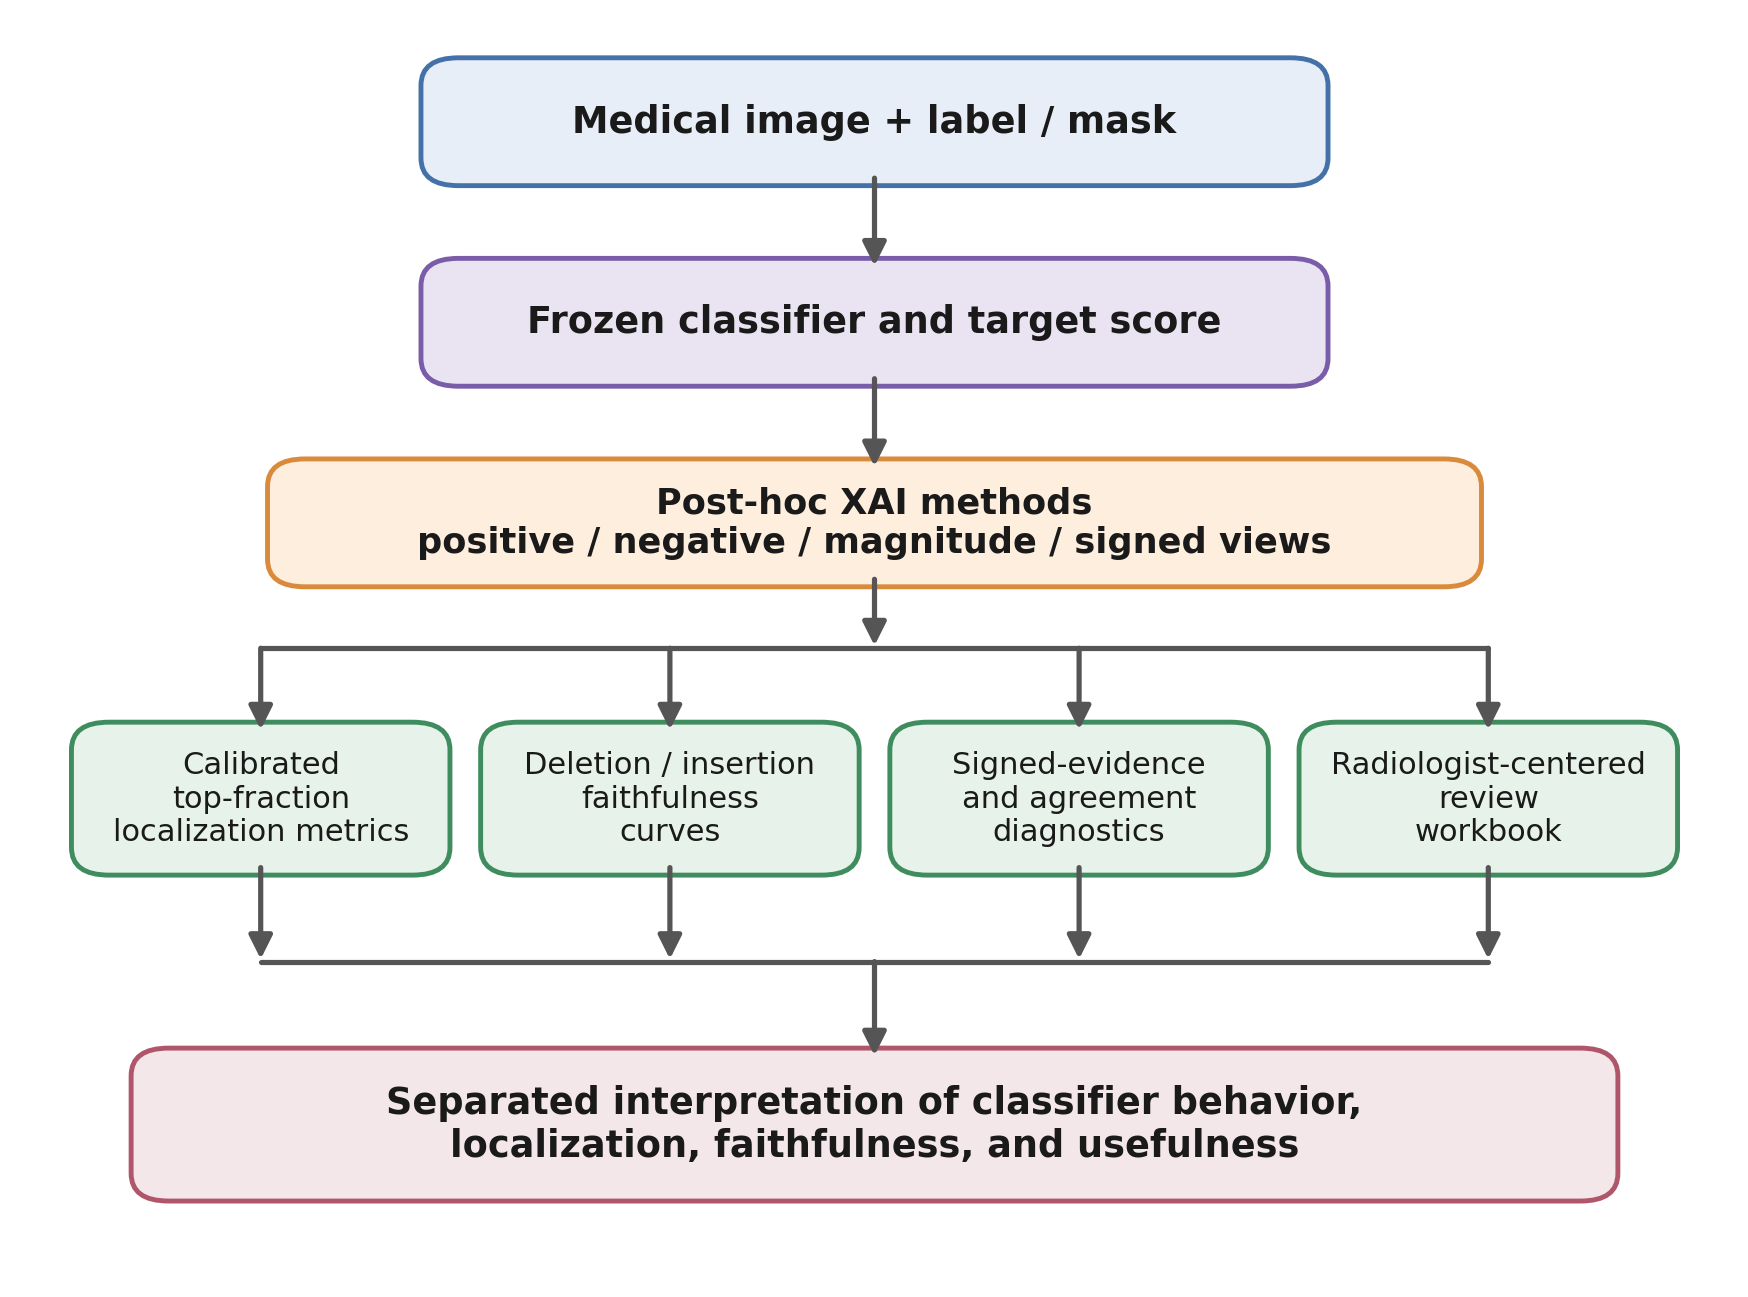
\includegraphics[width=0.92\linewidth,height=0.46\textheight,keepaspectratio]{figures/methodology_pipeline__figure_3_1.png}
	\caption{End-to-end validation pipeline used in this thesis.}
	\label{figure:3-1}
	\subcaption{A medical image with its label/mask is passed through a frozen classifier and target score, post-hoc XAI methods produce positive, negative, magnitude, and signed views, and these feed four parallel evaluation branches (calibrated top-fraction localization metrics, deletion/insertion faithfulness curves, signed-evidence and agreement diagnostics, and the radiologist-centered review workbook), whose outputs are interpreted separately for classifier behavior, localization, faithfulness, and usefulness.}
\end{figure}

\hypertarget{datasets}{%
	\section{Datasets}\label{datasets}}

\hypertarget{chest-x-ray-pneumothorax-dataset}{%
	\subsection{Chest X-ray pneumothorax
		dataset}\label{chest-x-ray-pneumothorax-dataset}}

The primary dataset is the local SIIM-ACR pneumothorax chest X-ray
snapshot \cite{ref-siim-acr}. The
working dataset state documented during this work contains
\texttt{12,\allowbreak 047} PNG images and \texttt{12,\allowbreak 047} corresponding PNG masks,
with \texttt{2,\allowbreak 669} positive pneumothorax cases and \texttt{9,\allowbreak 378}
negative cases. 

The dataset is used in two complementary ways. First, image-level labels
are used to screen classifier performance and define outcome groups
(\texttt{tp}, \texttt{fp}, \texttt{tn}, \texttt{fn}) at a frozen
classifier threshold. Second, positive masks are used for localization
evaluation of explanation maps. Negative images do not have lesion
masks; therefore, they are mainly used for classifier-outcome
visualization, false-positive analysis, and qualitative review rather
than Dice/IoU localization against a pneumothorax mask.

This study distinguishes calibration, exploratory, and held-out use.
Classifier-threshold and XAI top-fraction calibration must
not be tuned on final held-out test results. Current CXR work calibrates
the operating point per model on the training split. The selected
baselines use a TorchXRayVision pneumothorax cutoff of \texttt{0.\allowbreak 565}
for DenseNet-chex and \texttt{0.\allowbreak 525} for ResNet-50 (Table \ref{table:4-1}),
while the original DenseNet-all baseline used a higher cutoff of
approximately \texttt{0.\allowbreak 62}. Each cutoff was selected as the best
operating point for both F1 and Youden's J in the calibration
analysis.

\hypertarget{head-ct-hemorrhage-pilot-dataset}{%
	\subsection{Head CT hemorrhage pilot
		dataset}\label{head-ct-hemorrhage-pilot-dataset}}

The CT pilot uses the credentialed PhysioNet \texttt{ct-\allowbreak ich} v1.3.1
dataset \cite{ref-ct-ich, ref-physionet}. The dataset
contains NIfTI CT volumes and matched masks plus per-slice hemorrhage labels. The
verified local snapshot has \texttt{2,\allowbreak 814} slices, including
\texttt{318} hemorrhage-positive slices with masks and \texttt{2,\allowbreak 496}
normal slices. The final CT improvement experiment uses the train/test
split produced by the CT manifest builder: \texttt{213} positive train
slices for calibration and \texttt{105} positive test slices for
held-out evaluation.

Because the integrated CT classifier is a Vision Transformer, 
the explanation panel is restricted to the input-space
methods (Integrated Gradients, GradientSHAP,
Occlusion). These methods read only the model input and the
output score, so their implementations are model-agnostic and run with
identical code on the chest-X-ray and CT pipelines, which keeps the
cross-modality comparison controlled. CAM-family methods
 are not applied on the CT classifier: they weight a
two-dimensional convolutional activation map, and a Vision Transformer
\cite{ref-vit} instead represents the image as a sequence of patch
tokens with no such feature map. Running a CAM on a transformer would
require a token-to-grid reshape that constitutes a different explanation
technique;
transformer-native spatial-explanation methods such as attention rollout
\cite{ref-attention-rollout} or transformer attribution
\cite{ref-transformer-attribution} are therefore noted as future work. 
Because the frozen four-method consensus includes
Grad-CAM, it cannot be reproduced unchanged on the CT
classifier; any CT-side consensus is reported separately as an
exploratory aggregate over the three input-space methods.

\hypertarget{preprocessing}{%
	\section{Preprocessing}\label{preprocessing}}

For CXR experiments, each source image is loaded as a grayscale
radiograph and converted into the input format expected by the selected
classifier. TorchXRayVision preprocessing maps an \texttt{H\ x\ W} uint8
array in the range \texttt{0.\allowbreak .\allowbreak 255} through
\texttt{xrv.\allowbreak datasets.\allowbreak normalize(array,\allowbreak \ 255)} and returns a
single-channel tensor with shape \texttt{{[}1,\ H,\ W{]}}. The tensor is
then moved to the selected device. DenseNet-121 TorchXRayVision weights
are native to \texttt{224\ x\ 224} inputs, while the tested ResNet-50
TorchXRayVision weight \texttt{resnet50-\allowbreak res512-\allowbreak all} is native to
\texttt{512\ x\ 512}.

Masks are loaded as binary reference images for positive pneumothorax
cases. For mask-based metrics, heatmaps and masks are brought to the
same spatial grid before thresholding and comparison. Continuous
attribution maps are normalized only for visualization and selection;
normalization does not make them segmentations.

For CT, preprocessing does not reuse CXR normalization. CT images are
loaded from HU-preserving NIfTI volumes and rendered through a locked
brain window (\texttt{WL=40}, \texttt{WW=80}) before replication into
the three-channel format required by the DifeiT ViT image processor.
Perturbation baselines also differ: replacing CXR pixels with black is
not equivalent to replacing CT voxels with a meaningful HU value. For
the integrated DifeiT checkpoint, the image processor uses
\texttt{image \allowbreak mean\ =\ image \allowbreak std\ =\ 0.\allowbreak 5}, so the brain-window
midpoint maps to normalized value \texttt{0.\allowbreak 0}; in this specific model
contract, \texttt{brain \allowbreak window \allowbreak center} is numerically identical to
\texttt{zero \allowbreak tensor}, while black/air remains a separate stress-test
baseline.

All random sampling and balanced outcome selection use fixed seeds where
implemented. Stochastic explanation methods, especially GradientSHAP,
are reported with their sample count and noise settings. Broad
exploratory runs may use faster settings, while thesis-quality selected
cases are rerun with higher-stability settings.

\hypertarget{classification-models}{%
	\section{Classification Models}\label{classification-models}}

The CXR classifiers are loaded off-the-shelf from TorchXRayVision
\cite{ref-torchxrayvision}. The original baseline is
\texttt{DenseNet \allowbreak "densenet121-\allowbreak res224-\allowbreak all")}, used as
an external pretrained medical classifier without local modification,
fine-tuning, or forking. Thus weak SIIM
pneumothorax localization should not be interpreted as failure of a
locally optimized pneumothorax segmenter, but as evidence about transfer
behavior of a pretrained image-level classifier.

The CXR pipeline uses a classifier-loading seam, which returns the model,
Grad-CAM target layer, pneumothorax class index, and preprocessing
function. This allows model comparisons without changing downstream XAI
code. Current TorchXRayVision candidates include DenseNet-121 weights
such as \texttt{densenet121-\allowbreak res224-\allowbreak all},
\texttt{densenet121-\allowbreak res224-\allowbreak chex}, \texttt{densenet121-\allowbreak res224-\allowbreak mimic\_\allowbreak ch},
\texttt{densenet121-\allowbreak res224-\allowbreak mimic\_\allowbreak nb}, \texttt{densenet121-\allowbreak res224-\allowbreak rsna},
\texttt{densenet121-\allowbreak res224-\allowbreak nih}, and \texttt{densenet121-\allowbreak res224-\allowbreak pc},
plus the architecturally different \texttt{resnet50-\allowbreak res512-\allowbreak all}
classifier. The DenseNet Grad-CAM target layer is
\texttt{model.\allowbreak features.\allowbreak denseblock4}; for the TorchXRayVision ResNet-50
wrapper, the target layer is \texttt{model.\allowbreak model.\allowbreak layer4}.

The diagnostic model-comparison protocol treats
\texttt{densenet121-\allowbreak res224-\allowbreak all} as the control and asks whether poor
localization is stable across pretrained CXR weights or improves
materially for another model. The
\texttt{resnet50-\allowbreak res512-\allowbreak all} was selected as 
the strongest tested TorchXRayVision
follow-up candidate by aggregate localization, but absolute overlap
remained low; therefore it should be considered as a relative model-side
improvement, not as clinically sufficient localization.

The target output for all CXR explanations is the model's
\texttt{Pneumothorax} head. If a candidate model lacks a pneumothorax
class head, it is rejected for this pipeline rather than silently
attributing another class. Autoencoder-style weights are not valid
classifiers for this methodology.

\hypertarget{explainability-methods}{%
	\section{Explainability Methods}\label{explainability-methods}}

The explanation methods are post-hoc methods applied to an already
trained classifier. They are generated with respect to the selected
target score and are therefore class-specific attribution maps. The
current implementation for CXR includes Captum \cite{ref-captum-docs} and
pytorch-grad-cam \cite{ref-pytorch-gradcam} libraries:

\begin{itemize}
	\tightlist
	\item
	\textbf{Grad-CAM} \cite{ref-gradcam}: a
	class-discriminative activation-map method using gradients flowing
	into a final convolutional layer.
	\item
	\textbf{Grad-CAM++} 
	\cite{ref-gradcampp}: a CAM-family variant with modified
	activation-map weighting, included as a comparator rather than assumed
	to be universally superior.
	\item
	\textbf{Integrated Gradients} 
	\cite{ref-integrated-gradients}: a baseline-dependent path-integration
	attribution method. The number of integration steps and baseline
	choice must be reported.
	\item
	\textbf{GradientSHAP} \cite{ref-shap}: a
	stochastic additive-attribution approximation related to SHAP
	concepts. The number of samples, noise standard deviation, and
	stability settings must be reported.
	\item
	\textbf{Occlusion sensitivity} 
	\cite{ref-occlusion-zeiler}: a perturbation method that replaces local
	patches and measures the target-score response. Patch size, stride,
	and replacement baseline must be reported.
	\item
	\textbf{Eigen-CAM}  \cite{ref-eigen-cam}: a
	CAM-family method based on the first principal component of
	target-layer activations, included to broaden the activation-map
	comparison beyond gradient-weighted CAMs.
	\item
	\textbf{Score-CAM} \cite{ref-scorecam}: a
	CAM-family method that masks the input with normalized activation maps
	and weights them by signed target-logit changes relative to a
	baseline. It is computationally expensive because it requires
	additional forward passes; broad calibration runs therefore report the
	channel cap used for feasibility.
	\item
	\textbf{Consensus}: a sign-aware average of the
	frozen original constituent methods (Grad-CAM,
	Integrated Gradients, GradientSHAP, and
	Occlusion), used to test whether cross-method agreement
	produces a more stable explanation. Eigen-CAM and Score-CAM are
	deliberately reported as additional individual methods rather than
	being folded into the consensus definition, so that consensus results
	remain comparable across thesis iterations.
\end{itemize}

In turn, each method computes one normalized signed map and
derives four views from it:

\begin{itemize}
	\tightlist
	\item
	\texttt{positive}: non-negative evidence supporting the target score;
	\item
	\texttt{negative}: suppressive evidence against the target score;
	\item
	\texttt{magnitude}: absolute attribution strength, independent of
	direction;
	\item
	\texttt{signed}: the normalized signed map used for diverging overlays
	and signed diagnostics.
\end{itemize}

This design avoids recomputing the same method separately for each
polarity and makes the interpretation of positive, negative, magnitude,
and signed outputs explicit. For pixel-level methods such as Integrated
Gradients and GradientSHAP, optional smoothing may be applied for review
readability; if smoothing is used, metrics should be computed from the
same maps shown to the reviewer so that visualization and quantitative
evaluation remain aligned.

Figure~\ref{figure:3-2} illustrates the four-view contract used throughout the CXR
review workbook.

\begin{figure}[htbp]
	\centering
	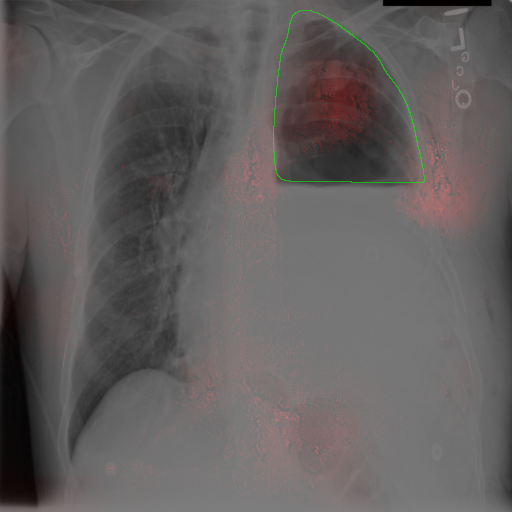
\includegraphics[width=0.237\linewidth,height=0.32\textheight,keepaspectratio]{figures/iter_48_resnet_review_workbook_balanced40_smoothed_faithfulness__review__assets__case_31__101_test_1__consensus_continuous_heatmap.png}%
	\hfill
	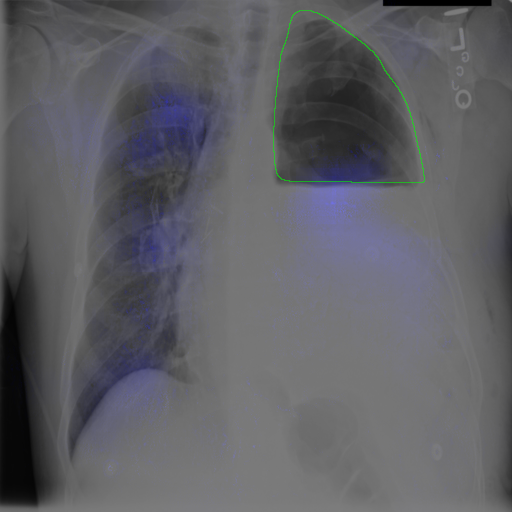
\includegraphics[width=0.237\linewidth,height=0.32\textheight,keepaspectratio]{figures/iter_48_resnet_review_workbook_balanced40_smoothed_faithfulness__review__assets__case_31__101_test_1__consensus_negative_continuous_heatmap.png}%
	\hfill
	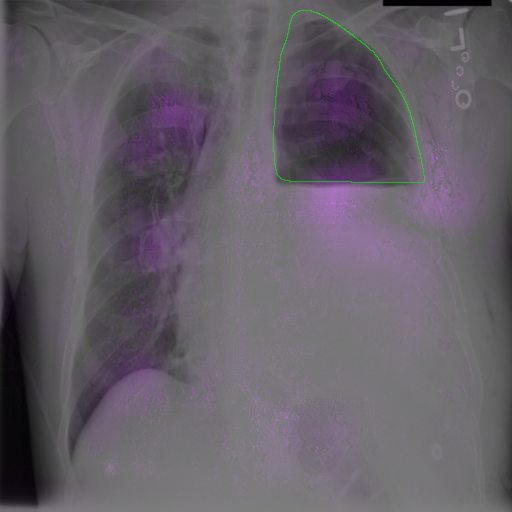
\includegraphics[width=0.237\linewidth,height=0.32\textheight,keepaspectratio]{figures/iter_48_resnet_review_workbook_balanced40_smoothed_faithfulness__review__assets__case_31__101_test_1__consensus_magnitude_continuous_heatmap.png}%
	\hfill
	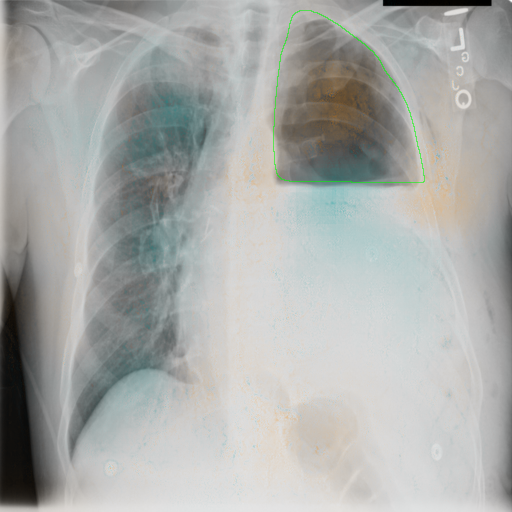
\includegraphics[width=0.237\linewidth,height=0.32\textheight,keepaspectratio]{figures/iter_48_resnet_review_workbook_balanced40_smoothed_faithfulness__review__assets__case_31__101_test_1__consensus_signed_continuous_heatmap.png}%
	\caption{Example four-view explanation contract for one review case}
	\label{figure:3-2}
\end{figure}

Table \ref{table:3-1} summarizes the method panel and the semantic role of each
output view.

\begin{longtable}[]{@{}llll@{}}
	\caption{Method panel and explanation-view semantics}\tabularnewline
	\toprule
	\begin{minipage}[b]{0.17\columnwidth}\raggedright
		Method family\strut
	\end{minipage} & \begin{minipage}[b]{0.17\columnwidth}\raggedright
		Method\strut
	\end{minipage} & \begin{minipage}[b]{0.17\columnwidth}\raggedright
		Primary evidence type\strut
	\end{minipage} & \begin{minipage}[b]{0.17\columnwidth}\raggedright
		Final parameter fields to report\strut
	\end{minipage}\tabularnewline
	\midrule
	\endfirsthead
	\toprule
	\begin{minipage}[b]{0.17\columnwidth}\raggedright
		Method family\strut
	\end{minipage} & \begin{minipage}[b]{0.17\columnwidth}\raggedright
		Method\strut
	\end{minipage} & \begin{minipage}[b]{0.17\columnwidth}\raggedright
		Primary evidence type\strut
	\end{minipage} & \begin{minipage}[b]{0.17\columnwidth}\raggedright
		Final parameter fields to report\strut
	\end{minipage}\tabularnewline
	\midrule
	\endhead
	\begin{minipage}[t]{0.17\columnwidth}\raggedright
		Grad-CAM\strut
	\end{minipage} & \begin{minipage}[t]{0.17\columnwidth}\raggedright
		Grad-CAM\strut
	\end{minipage} & \begin{minipage}[t]{0.17\columnwidth}\raggedright
		target-layer gradient-weighted activation evidence\strut
	\end{minipage} & \begin{minipage}[t]{0.17\columnwidth}\raggedright
		target layer, input size\strut
	\end{minipage}\tabularnewline
	\begin{minipage}[t]{0.17\columnwidth}\raggedright
		Grad-CAM++\strut
	\end{minipage} & \begin{minipage}[t]{0.17\columnwidth}\raggedright
		Grad-CAM++\strut
	\end{minipage} & \begin{minipage}[t]{0.17\columnwidth}\raggedright
		CAM variant with modified gradient weighting\strut
	\end{minipage} & \begin{minipage}[t]{0.17\columnwidth}\raggedright
		target layer, input size\strut
	\end{minipage}\tabularnewline
	\begin{minipage}[t]{0.17\columnwidth}\raggedright
		Integrated Gradients\strut
	\end{minipage} & \begin{minipage}[t]{0.17\columnwidth}\raggedright
		Integrated Gradients\strut
	\end{minipage} & \begin{minipage}[t]{0.17\columnwidth}\raggedright
		baseline-dependent pixel attribution\strut
	\end{minipage} & \begin{minipage}[t]{0.17\columnwidth}\raggedright
		baseline, \texttt{ig\_\allowbreak steps}, smoothing if used\strut
	\end{minipage}\tabularnewline
	\begin{minipage}[t]{0.17\columnwidth}\raggedright
		GradientSHAP\strut
	\end{minipage} & \begin{minipage}[t]{0.17\columnwidth}\raggedright
		GradientSHAP\strut
	\end{minipage} & \begin{minipage}[t]{0.17\columnwidth}\raggedright
		stochastic baseline/noise pixel attribution\strut
	\end{minipage} & \begin{minipage}[t]{0.17\columnwidth}\raggedright
		samples, stdevs, seed, smoothing if used\strut
	\end{minipage}\tabularnewline
	\begin{minipage}[t]{0.17\columnwidth}\raggedright
		Occlusion\strut
	\end{minipage} & \begin{minipage}[t]{0.17\columnwidth}\raggedright
		Occlusion\strut
	\end{minipage} & \begin{minipage}[t]{0.17\columnwidth}\raggedright
		patch perturbation sensitivity\strut
	\end{minipage} & \begin{minipage}[t]{0.17\columnwidth}\raggedright
		patch size, stride, baseline\strut
	\end{minipage}\tabularnewline
	\begin{minipage}[t]{0.17\columnwidth}\raggedright
		Eigen-CAM\strut
	\end{minipage} & \begin{minipage}[t]{0.17\columnwidth}\raggedright
		Eigen-CAM\strut
	\end{minipage} & \begin{minipage}[t]{0.17\columnwidth}\raggedright
		activation principal-component map\strut
	\end{minipage} & \begin{minipage}[t]{0.17\columnwidth}\raggedright
		target layer, sign-orientation rule\strut
	\end{minipage}\tabularnewline
	\begin{minipage}[t]{0.17\columnwidth}\raggedright
		Score-CAM\strut
	\end{minipage} & \begin{minipage}[t]{0.17\columnwidth}\raggedright
		Score-CAM\strut
	\end{minipage} & \begin{minipage}[t]{0.17\columnwidth}\raggedright
		activation-mask forward-pass scoring\strut
	\end{minipage} & \begin{minipage}[t]{0.17\columnwidth}\raggedright
		target layer, channel cap, baseline\strut
	\end{minipage}\tabularnewline
	\begin{minipage}[t]{0.17\columnwidth}\raggedright
		Frozen consensus\strut
	\end{minipage} & \begin{minipage}[t]{0.17\columnwidth}\raggedright
		consensus\strut
	\end{minipage} & \begin{minipage}[t]{0.17\columnwidth}\raggedright
		average of original four constituent methods\strut
	\end{minipage} & \begin{minipage}[t]{0.17\columnwidth}\raggedright
		constituent list, signed-map normalization\strut
	\end{minipage}\tabularnewline
	\bottomrule
	\label{table:3-1}
\end{longtable}

\hypertarget{explanation-validation-metrics}{%
	\section{Explanation Validation
		Metrics}\label{explanation-validation-metrics}}

The validation protocol intentionally combines multiple metrics because
explanation quality has no single ground truth. Mask-overlap,
peak-localization, negative-evidence, faithfulness, and review-score
measures answer different questions.

\hypertarget{top-fraction-selection}{%
	\subsection{Top-fraction selection}\label{top-fraction-selection}}

Continuous heatmaps are converted to binary selected regions using
top-fraction thresholding. Given a fraction \texttt{f}, the pipeline
keeps the highest-valued \texttt{f} proportion of pixels after
normalization. The selected region is then compared with the binary
lesion mask. The fraction can be fixed, swept across values, or selected
from calibration. Current useful sweep values are \texttt{0.\allowbreak 05} to
\texttt{0.\allowbreak 95} in increments of \texttt{0.\allowbreak 05}. Broad visualization sweeps
stop after selected-image coverage reaches approximately \texttt{0.\allowbreak 95}
to avoid redundant whole-image panels.

\hypertarget{positive-localization-metrics}{%
	\subsection{Positive localization
		metrics}\label{positive-localization-metrics}}

For positive-label cases with masks, the primary localization metrics
are:

\begin{itemize}
	\tightlist
	\item
	\textbf{Intersection over Union (IoU)}: the intersection of selected
	explanation pixels (P) and mask pixels (GT) divided by their union, as in formula \eqref{eq:3-1}.
	\begin{equation}
		\text{IoU} = \frac{|GT \cap P|}{|GT \cup P|}
		\label{eq:3-1}
	\end{equation}
	\item
	\textbf{Dice-Soerensen score}: twice the intersection divided by the sum of
	selected pixels (P) and mask pixels (GT), as in formula \eqref{eq:3-2}.
	\begin{equation}
		\text{Dice} = \frac{2 \cdot |GT \cap P|}{|GT| + |P|}
		\label{eq:3-2}
	\end{equation}
	\item
	\textbf{Pointing Game hit (or pointing hit)}: \texttt{1} if the maximum-attribution pixel
	lies inside the lesion mask, otherwise \texttt{0}, as in formula \eqref{eq:3-3}.
	\begin{equation}
		H(A, M) = \begin{cases} 
			1 & \text{if } \arg\max_{(i,j)} A_{i,j} \in M \\ 
			0 & \text{otherwise} 
		\end{cases}
		\label{eq:3-3}
	\end{equation}
	\begin{center}
		\small
		\begin{tabular}{lp{9cm}}
			\toprule
			\textbf{Symbol} & \textbf{Description} \\
			\midrule
			$A$ & The normalized attribution map or heatmap generated by the explanation method. \\
			$(i^*, j^*)$ & The coordinates of the maximum-attribution pixel, defined as $\arg\max_{(i,j)} A_{i,j}$, representing the peak focus of the model's decision. \\
			$M$ & The binary ground-truth lesion mask, where $M_{i,j} = 1$ inside the lesion and $0$ otherwise. \\
			\bottomrule
		\end{tabular}
	\end{center}
	\item
	\textbf{Precision at fraction (\texttt{P@F})}: the proportion of selected
	top-fraction pixels that fall inside the mask, as in formula \eqref{eq:3-4}.
	\begin{equation}
		\text{P@F}(A, M) = \frac{|P_f \cap M|}{|P_f|} = \frac{\sum_{(i,j) \in P_f} M_{i,j}}{|P_f|}
		\label{eq:3-4}
	\end{equation}
	\begin{center}
		\small
		\begin{tabular}{lp{9cm}}
			\toprule
			\textbf{Symbol} & \textbf{Description} \\
			\midrule
			$A$ & The continuous attribution map (saliency map) generated by the explanation method. \\
			$M$ & The binary ground-truth lesion mask, where $M_{i,j} = 1$ inside the lesion and $0$ otherwise. \\
			$f$ & The fraction or proportion of top pixels to be selected (e.g., $f = 0.05$ for the top 5\%). \\
			$P_f$ & The set of pixels containing the highest attribution values in $A$, such that the cardinality $|P_f| = f \times N$, where $N$ is the total number of pixels in the image. \\
			$|P_f \cap M|$ & The number of selected top-fraction pixels that fall inside the lesion mask. \\
			\bottomrule
		\end{tabular}
	\end{center}
\end{itemize}

IoU, Dice, and \texttt{P@F} primarily measure overlap. Pointing
hit measures whether the single strongest attribution point falls inside
the lesion and should not be treated as interchangeable with overlap
metrics. Current evidence in this study suggests that overlap metrics can be
highly correlated with each other while pointing hit captures a stricter
peak-localization property.

\hypertarget{negative-evidence-diagnostics}{%
	\subsection{Negative-evidence
		diagnostics}\label{negative-evidence-diagnostics}}

Negative evidence is not evaluated as if lesion overlap were
automatically desirable. For a negative view, selected pixels inside the
pneumothorax mask can mean that the model is treating lesion-region
information as suppressive evidence, which may be clinically concerning.
The pipeline therefore reports:

\begin{itemize}
	\tightlist
	\item
	\textbf{negative mask overlap fraction}: the fraction of selected
	negative-evidence pixels inside the lesion mask;
	\item
	\textbf{negative mask avoidance fraction}:
	\texttt{1\ -\allowbreak \ negative \allowbreak mask \allowbreak overlap \allowbreak fraction}, interpreted as how
	much selected negative evidence avoids the lesion.
\end{itemize}

These metrics are diagnostics rather than universal correctness scores.
They are interpreted together with the classifier outcome, positive
localization, and visual review.

\hypertarget{faithfulness-curves}{%
	\subsection{Faithfulness curves}\label{faithfulness-curves}}

Faithfulness is evaluated by perturbing the actual model input according
to each attribution ranking and re-evaluating the classifier probability
\cite{ref-rise, ref-samek-evaluation}. In a deletion curve, pixels are
removed or replaced from the original image in descending attribution
order; a faithful positive explanation is expected to reduce the target
probability quickly. In an insertion curve, pixels are restored into a
baseline image in descending attribution order; a faithful explanation
is expected to recover the target probability quickly. 
Rapid decline (in deletion) and elevation (in insertion) of the same threshold
amount of pixels is considered important for the model
decision and as such gives a signal-to-noise differentiation for XAI maps.

For current CXR faithfulness runs, the preferred baseline is a true
black-image baseline in the normalized TorchXRayVision input space.
The \texttt{zero \allowbreak tensor} baselines were found to be misleading
because they could still produce high pneumothorax probabilities.
Faithfulness curves are reported as model-behavior tests: a method may
be faithful to the classifier while remaining clinically poorly
localized against the pneumothorax mask. Faithfulness is evaluated per
case with deletion and insertion curves and interpreted alongside the
localization metrics in Section~\ref{quantitative-explanation-validation},
where the ResNet-50 curves are reported; the CT hemorrhage curves are
shown in Appendix~\ref{additional-figures} (Figure~\ref{figure:c-4}).

\hypertarget{spatial-saturation-and-agreement-diagnostics}{%
	\subsection{Spatial saturation and agreement
		diagnostics}\label{spatial-saturation-and-agreement-diagnostics}}

The proposed secondary coverage metric,
\texttt{coverage \allowbreak saturation \allowbreak fraction \allowbreak at 95}, records the smallest swept
top-fraction at which the selected explanation region covers at least
\texttt{95\%} of the image. It is used only as a spatial diffuseness or
saturation diagnostic. Lower values indicate that the thresholded map
becomes whole-image-like quickly; higher values indicate that
attribution remains more spatially concentrated over the tested
fractions. It does not decide whether positive or negative evidence is
clinically correct. However, it may be used as an evidence of either positive 
or negative map has more strength or impact, if it takes more time to
diffuse. The faster diffusion can be interpreted as a sign that the overall 
impact level is low.

Signed-capable runs may also report method-agreement diagnostics, such
as cosine similarity between signed maps. Agreement between methods is
treated as stronger evidence than a single overlay, while disagreement
is useful for detecting instability, baseline sensitivity, or reliance
on non-lesion cues.

\hypertarget{calibration-and-paired-statistical-comparison}{%
	\subsection{Calibration and paired statistical
		comparison}\label{calibration-and-paired-statistical-comparison}}

Classifier thresholds and explanation thresholds are calibrated
separately. The classifier threshold converts the pneumothorax
probability into an image-level outcome (\texttt{tp}, \texttt{fp},
\texttt{tn}, or \texttt{fn}). The selection criteria use both the F1 score (formula \eqref{eq:3-5})
and Youden's J (formula \eqref{eq:3-6}) statistic to identify the threshold candidate with the
best performance.

\begin{equation}
	F_1 = 2 \times \frac{\text{Precision} \times \text{Recall}}{\text{Precision} + \text{Recall}} = \frac{2\text{TP}}{2\text{TP} + \text{FP} + \text{FN}}
	\label{eq:3-5}
\end{equation}

\begin{equation}
	J = \text{Sensitivity} + \text{Specificity} - 1
	\label{eq:3-6}
\end{equation}

In contrast, the XAI top-fraction
threshold selects a spatial region from each heatmap for mask
comparison. Tuning one threshold does not tune the other, and neither
should be optimized on the final held-out test results.

The improvement experiment compares the frozen four-method consensus
against each individual method using paired case-level metrics
\cite{ref-demsar-2006}. The primary statistical test is the Wilcoxon
signed-rank test \cite{ref-wilcoxon-1945}, chosen because localization
scores are bounded, as in formula \eqref{eq:3-7}, often zero-inflated, and not safely assumed to be
normally distributed. 

\begin{equation}
	W = \min \left( \sum_{i=1}^{N_r} \text{sgn}(x_{1,i} - x_{2,i}) \cdot R_i , \quad \sum_{i=1}^{N_r} I(x_{1,i} - x_{2,i} < 0) \cdot R_i \right)
	\label{eq:3-7}
\end{equation}
\begin{center}
	\small
	\begin{tabular}{lp{9cm}}
		\toprule
		\textbf{Symbol} & \textbf{Description} \\
		\midrule
		$x_{1,i}, x_{2,i}$ & The paired observations from the first and second sample (or metric scores) for the $i$-th subject. \\
		$x_{1,i} - x_{2,i}$ & The difference between the $i$-th pair. Pairs with a difference of zero are excluded from the analysis. \\
		$N_r$ & The reduced sample size, representing the total number of pairs remaining after excluding pairs with zero difference. \\
		$R_i$ & The rank assigned to the absolute difference $|x_{1,i} - x_{2,i}|$. Smallest absolute differences receive the lowest ranks. \\
		$\text{sgn}(x)$ & The sign function, returning $+1$ if $x > 0$, $-1$ if $x < 0$, and $0$ if $x = 0$. \\
		$\text{sgn}^+(x)$ & An indicator function that returns $1$ if $x > 0$ and $0$ otherwise, used to sum only the positive ranks. \\
		\bottomrule
	\end{tabular}
\end{center}

Multiple consensus-vs-method comparisons are
corrected with Holm-Bonferroni family-wise error control
\cite{ref-holm-1979, ref-aickin-gensler-1996} at
\texttt{alpha\ =\ 0.\allowbreak 05}, as formula \eqref{eq:3-8}. 

\begin{equation}
	p_i \le \frac{\alpha}{m - i + 1}
	\label{eq:3-8}
\end{equation}

\begin{center}
	\small
	\begin{tabular}{lp{9cm}}
		\toprule
		\textbf{Symbol} & \textbf{Description} \\
		\midrule
		$p_i$ & The $i$-th smallest uncorrected $p$-value from the set of comparisons. \\
		$\alpha$ & The nominal family-wise significance level, set to $\alpha = 0.05$. \\
		$m$ & The total number of statistical hypotheses (comparisons) being tested. \\
		$i$ & The current rank index of the sorted $p$-value being evaluated. \\
		$m - i + 1$ & The remaining number of hypotheses to be tested at step $i$, adjusting the penalty strictly for each step. \\
		\bottomrule
	\end{tabular}
\end{center}

The effect-size companion is the median paired
difference with a bootstrap 95\% confidence interval under a fixed seed.
This framing separates statistical evidence for paired improvement from
visual or clinical usefulness, which is still assessed through
representative cases and the radiologist-centered review.

Table \ref{table:3-2} records the intended calibration and held-out evaluation
discipline, while table \ref{table:3-3} provides a compact metric interpretation guide

\begin{longtable}[]{@{}llll@{}}
	\caption{Calibration and held-out evaluation protocol}\tabularnewline
	\toprule
	\begin{minipage}[b]{0.17\columnwidth}\raggedright
		Stage\strut
	\end{minipage} & \begin{minipage}[b]{0.17\columnwidth}\raggedright
		Data used\strut
	\end{minipage} & \begin{minipage}[b]{0.17\columnwidth}\raggedright
		Output artifact\strut
	\end{minipage} & \begin{minipage}[b]{0.17\columnwidth}\raggedright
		Purpose\strut
	\end{minipage} \tabularnewline
	\midrule
	\endfirsthead
	\toprule
	\begin{minipage}[b]{0.17\columnwidth}\raggedright
		Stage\strut
	\end{minipage} & \begin{minipage}[b]{0.17\columnwidth}\raggedright
		Data used\strut
	\end{minipage} & \begin{minipage}[b]{0.17\columnwidth}\raggedright
		Output artifact\strut
	\end{minipage} & \begin{minipage}[b]{0.17\columnwidth}\raggedright
		Purpose\strut
	\end{minipage} \tabularnewline
	\midrule
	\endhead
	\begin{minipage}[t]{0.17\columnwidth}\raggedright
		Classifier threshold calibration\strut
	\end{minipage} & \begin{minipage}[t]{0.17\columnwidth}\raggedright
		train/calibration subset\strut
	\end{minipage} & \begin{minipage}[t]{0.17\columnwidth}\raggedright
		selected probability cutoff per model\strut
	\end{minipage} & \begin{minipage}[t]{0.17\columnwidth}\raggedright
		define \texttt{tp}/\texttt{fp}/\texttt{tn}/\texttt{fn} outcomes\strut
	\end{minipage}\tabularnewline
	\begin{minipage}[t]{0.17\columnwidth}\raggedright
		XAI top-fraction calibration\strut
	\end{minipage} & \begin{minipage}[t]{0.17\columnwidth}\raggedright
		positive masked train-split cases\strut
	\end{minipage} & \begin{minipage}[t]{0.17\columnwidth}\raggedright
		\texttt{calibrated \allowbreak thresholds} per model\strut
	\end{minipage} & \begin{minipage}[t]{0.17\columnwidth}\raggedright
		choose method/view fractions for spatial metrics\strut
	\end{minipage} \tabularnewline
	\begin{minipage}[t]{0.17\columnwidth}\raggedright
		Improvement experiment\strut
	\end{minipage} & \begin{minipage}[t]{0.17\columnwidth}\raggedright
		positive masked test-split cases\strut
	\end{minipage} & \begin{minipage}[t]{0.17\columnwidth}\raggedright
		\texttt{improvement \allowbreak experiment}, paired statistics, plots\strut
	\end{minipage} & \begin{minipage}[t]{0.17\columnwidth}\raggedright
		compare consensus against individual methods\strut
	\end{minipage} \tabularnewline
	\begin{minipage}[t]{0.17\columnwidth}\raggedright
		Qualitative review\strut
	\end{minipage} & \begin{minipage}[t]{0.17\columnwidth}\raggedright
		balanced selected cases\strut
	\end{minipage} & \begin{minipage}[t]{0.17\columnwidth}\raggedright
		review workbook and scores\strut
	\end{minipage} & \begin{minipage}[t]{0.17\columnwidth}\raggedright
		assess usefulness and failure modes\strut
	\end{minipage} \tabularnewline
	\bottomrule
	\label{table:3-2}
\end{longtable}

\begin{longtable}[]{@{}llll@{}}
	\caption{Metric interpretation guide for localization, faithfulness, and
		review scores}\tabularnewline
	\toprule
	\begin{minipage}[b]{0.22\columnwidth}\raggedright
		Evidence layer\strut
	\end{minipage} & \begin{minipage}[b]{0.22\columnwidth}\raggedright
		Metric or artifact\strut
	\end{minipage} & \begin{minipage}[b]{0.22\columnwidth}\raggedright
		What higher/better means\strut
	\end{minipage} & \begin{minipage}[b]{0.22\columnwidth}\raggedright
		What it does not prove\strut
	\end{minipage}\tabularnewline
	\midrule
	\endfirsthead
	\toprule
	\begin{minipage}[b]{0.22\columnwidth}\raggedright
		Evidence layer\strut
	\end{minipage} & \begin{minipage}[b]{0.22\columnwidth}\raggedright
		Metric or artifact\strut
	\end{minipage} & \begin{minipage}[b]{0.22\columnwidth}\raggedright
		What higher/better means\strut
	\end{minipage} & \begin{minipage}[b]{0.22\columnwidth}\raggedright
		What it does not prove\strut
	\end{minipage}\tabularnewline
	\midrule
	\endhead
	\begin{minipage}[t]{0.22\columnwidth}\raggedright
		Positive localization\strut
	\end{minipage} & \begin{minipage}[t]{0.22\columnwidth}\raggedright
		\texttt{IoU}, \texttt{Dice}, \texttt{precision\allowbreak at\allowbreak fraction}\strut
	\end{minipage} & \begin{minipage}[t]{0.22\columnwidth}\raggedright
		there is a higher overlap of selected positive evidence with the pneumothorax mask\strut
	\end{minipage} & \begin{minipage}[t]{0.22\columnwidth}\raggedright
		the model is clinically safe or the heatmap is non-diagnostic\strut
	\end{minipage}\tabularnewline
	\begin{minipage}[t]{0.22\columnwidth}\raggedright
		Peak localization\strut
	\end{minipage} & \begin{minipage}[t]{0.22\columnwidth}\raggedright
		\texttt{pointing \allowbreak hit}\strut
	\end{minipage} & \begin{minipage}[t]{0.22\columnwidth}\raggedright
		the maximum-attribution pixel lies inside the lesion mask\strut
	\end{minipage} & \begin{minipage}[t]{0.22\columnwidth}\raggedright
		broad map quality or overall lesion coverage\strut
	\end{minipage}\tabularnewline
	\begin{minipage}[t]{0.22\columnwidth}\raggedright
		Negative diagnostics\strut
	\end{minipage} & \begin{minipage}[t]{0.22\columnwidth}\raggedright
		\texttt{negative \allowbreak mask \allowbreak avoidance \allowbreak fraction}\strut
	\end{minipage} & \begin{minipage}[t]{0.22\columnwidth}\raggedright
		the qualitative characteristic of how much the selected negative 
		evidence avoids the lesion mask\strut
	\end{minipage} & \begin{minipage}[t]{0.22\columnwidth}\raggedright
		clinical correctness or relevance\strut
	\end{minipage}\tabularnewline
	\begin{minipage}[t]{0.22\columnwidth}\raggedright
		Faithfulness\strut
	\end{minipage} & \begin{minipage}[t]{0.22\columnwidth}\raggedright
		deletion/insertion curves and AUC\strut
	\end{minipage} & \begin{minipage}[t]{0.22\columnwidth}\raggedright
		highlighted pixels affect the model probability output under the chosen
		perturbation, i.e. the selected fraction is important for the model
		decision - signal-to-noise differentiation for XAI maps\strut
	\end{minipage} & \begin{minipage}[t]{0.22\columnwidth}\raggedright
		highlighted pixels are clinically appropriate pathology evidence\strut
	\end{minipage}\tabularnewline
	\begin{minipage}[t]{0.22\columnwidth}\raggedright
		Method agreement\strut
	\end{minipage} & \begin{minipage}[t]{0.22\columnwidth}\raggedright
		signed-map cosine similarity or qualitative agreement\strut
	\end{minipage} & \begin{minipage}[t]{0.22\columnwidth}\raggedright
		multiple methods highlight similar signed evidence\strut
	\end{minipage} & \begin{minipage}[t]{0.22\columnwidth}\raggedright
		the shared evidence is lesion-aligned\strut
	\end{minipage}\tabularnewline
	\begin{minipage}[t]{0.22\columnwidth}\raggedright
		Human-centered review\strut
	\end{minipage} & \begin{minipage}[t]{0.22\columnwidth}\raggedright
		localization/usefulness/failure taxonomy\strut
	\end{minipage} & \begin{minipage}[t]{0.22\columnwidth}\raggedright
		a medically trained reviewer finds the explanation useful or identifies
		a failure mode\strut
	\end{minipage} & \begin{minipage}[t]{0.22\columnwidth}\raggedright
		prospective deployment safety or inter-rater reliability\strut
	\end{minipage}\tabularnewline
	\bottomrule
	\label{table:3-3}
\end{longtable}

\hypertarget{radiologist-centered-assessment}{%
	\section{Radiologist-Centered
		Assessment}\label{radiologist-centered-assessment}}

The radiologist-centered component is implemented as a static review
workbook generated from selected rendered cases. The workbook is
designed for a controlled review task rather than for
clinical deployment. Each case card shows the source CXR, ground-truth
mask where available, classifier outcome and probability, and a grid of
explanation overlays. Current review workbooks include method rows and
four views per method so that positive, negative, magnitude, and signed
evidence can be inspected separately.

The scoring schema contains four fields:

\begin{itemize}
	\tightlist
	\item
	\texttt{localization \allowbreak score} 
	\subitem
	evaluates how well does the heatmap localize the target lesion
	\subitem options are \texttt{\{correct,\allowbreak \ partial,\allowbreak \ incorrect,\allowbreak \ none\}};
	\item
	\texttt{usefulness \allowbreak score} 
	\subitem 
	evaluates how useful the mask maps to identify the clinical correctness and/or the failure reason
	\subitem options are \texttt{\{useful,\allowbreak \ potentially \allowbreak useful,\allowbreak \ misleading,\allowbreak \ not \allowbreak useful\}};
	\item
	\texttt{failure \allowbreak category} 
	\subitem
	describes the primary or most impactful reason why the masks may show incorrect information based on XAI perturbation
	\subitem options are \texttt{\{correct,\allowbreak \ partial,\allowbreak \ anatomically \allowbreak related,\allowbreak \ devices \allowbreak and text \allowbreak artifacts,\allowbreak \ non \allowbreak pathological \allowbreak high \allowbreak contrast,\allowbreak \ diffuse \allowbreak non \allowbreak specific,\allowbreak \ clinically \allowbreak misleading\}};
	\item
	free-text \texttt{artifact \allowbreak note} and \texttt{comment} fields.
\end{itemize}

The review design follows human-centered XAI principles
\cite{ref-human-centered-xai}: the intended user is a board-certified radiologist
reviewer, the task is explanation assessment rather than diagnosis, and
all scoring categories are visible in the workbook to reduce context
switching. The workbook includes instructions and warmup guidance so
that scoring is anchored before the main review pass.
Classifier-outcome-balanced selections preserve \texttt{tp},
\texttt{fp}, \texttt{tn}, and \texttt{fn} examples where possible,
because explanation failures can differ across successful predictions,
false alarms, and missed positives.

Review scores are interpreted as structured qualitative evidence. They
do not replace quantitative localization or faithfulness metrics.
In this work the author -- a radiologist with five years of
experience at a high-volume trauma center -- performed a single-reader
evaluation of 40 cases. This single-reader review is not presented 
as prospective clinical 
validation. The review is nevertheless important because masks do not
capture every clinically relevant pattern: devices, drains, subcutaneous
emphysema, image markers, and indirect signs that can be clinically related
or confounding even when they do not overlap the pneumothorax mask.

\hypertarget{ethical-and-practical-considerations}{%
	\section{Ethical and Practical
		Considerations}\label{ethical-and-practical-considerations}}

The experiments use public retrospective medical-imaging data
and do not alter patient care. Public CXR data are treated as
de-identified challenge data, and local data is not committed as source artifacts.
Generated figures avoid patient-identifiable metadata and use source image 
stems only for traceability within the experiment folders.

The head CT hemorrhage data are the
PhysioNet Computed Tomography Images for Intracranial Hemorrhage
Detection and Segmentation dataset (version 1.3.1). These are restricted health data and 
were obtained under the PhysioNet Restricted
Health Data Use Agreement 1.5.0. In accordance with that agreement, the
author made no attempt to identify any individual or institution
referenced in the data, exercised reasonable and prudent care to
maintain the physical and electronic security of the data, did not share
access to the data with any other party, and used the data solely for
lawful scientific research. Consistent with these terms, the restricted
CT data are not redistributed with this thesis or its code; only
derived, non-identifiable artifacts (such as aggregate metrics and
example visualizations with masking) are reported. The analysis code
associated with this work is openly released to the research community
(see Section~\ref{implementation-and-reproducibility}), while the
restricted datasets themselves are not redistributed.

\hypertarget{implementation-and-reproducibility}{%
	\section{Implementation and
		Reproducibility}\label{implementation-and-reproducibility}}

The CXR pipeline is organized as a sequence of reusable stages built on
shared package modules. A classifier-screening stage calculates each
TorchXRayVision baseline on the test split and records image-level
ranking metrics. An explanation stage calculates the attribution methods and
the frozen consensus over the selected positive views. A calibration
stage estimates per-method top-fraction thresholds on the training
split, and dedicated diagnostic stages produce single-case threshold
 and outcome-balanced visualizations grouped by
classifier outcome. A final review stage prepares the structured
radiologist-review workbook from the calibrated explanations.

Each stage writes its results to a self-contained, ordinally named
experiment folder: root-level CSV summaries are kept at the run root,
and image artifacts are grouped by case so that exported heatmaps remain
traceable to their source slice. For the classifier-outcome
visualizations, TP, FP, TN, FN groupings are preserved as separate subfolders. The
complete manifest maps every reported experiment to its run folder
is given in Appendix~\ref{experiment-configuration}.

The codebase is covered by an automated test suite including 
package modules and output schemas. The complete analysis code is
publicly available on GitHub.\footnote{\url{https://github.com/dem-v/Capstone_project}.
Accessed: 15 June 2026.}

\hypertarget{conclusions-to-chapter-3}{%
	\section*{Conclusions to Chapter 3}\label{conclusions-to-chapter-3}}
\addcontentsline{toc}{section}{Conclusions to Chapter 3}

The methodology defines XAI validation as a layered experimental problem. 
The classifier layer
measures whether an off-the-shelf medical image classifier assigns the
correct image-level pneumothorax label. The localization layer tests
whether selected attribution regions overlap available pneumothorax
masks. The faithfulness layer asks whether perturbing highly attributed
pixels changes the actual model probability in the expected direction.
The human-centered layer then checks whether a medically trained
reviewer finds the explanations useful, misleading, or clinically
incomplete under a defined scoring rubric. Keeping these layers separate
is essential because a heatmap can be faithful to the model while still
being poorly localized to clinically expected pathology.

The CXR pipeline uses TorchXRayVision classifiers without local
fine-tuning. DenseNet-all remains the original historical 
baseline, but the diagnostic sweep identified DenseNet-chex as
the stronger DenseNet-121 checkpoint, and ResNet-50 as the strongest
tested TorchXRayVision model overall. Explanation methods are
implemented through the \texttt{Signed Attribution} contract, which
provides positive, negative, magnitude, and signed views from one
underlying attribution map. The method panel includes CAM-family,
pixel-attribution, perturbation, and consensus approaches; as well as 
Eigen-CAM and Score-CAM additions as individual methods.

The evaluation protocol protects the train/test boundary by separating
classifier-threshold calibration, XAI top-fraction calibration, and
testing. Wilcoxon signed-rank tests,
Holm-Bonferroni correction, and bootstrap confidence intervals provide a
non-parametric statistical framework for consensus-vs-individual
comparisons. The scripts, output folder structure, seeds, and run metadata make
the experiments reproducible.

\hypertarget{results-and-discussion}{%
	\chapter{Results and Discussion}\label{results-and-discussion}}

\hypertarget{classification-performance}{%
	\section{Classification Performance}\label{classification-performance}}

Classifier screening confirms that the selected CXR baselines differ
substantially in image-level ranking performance. DenseNet-chex replaces
DenseNet-all as the current DenseNet baseline because the diagnostic
model-comparison sweep showed
better aggregate localization among DenseNet-121 checkpoints; the full
CheX test screen shows moderate
image-level performance but not a uniformly better classifier-ranking
profile than the original DenseNet-all. ResNet-50 is a stronger
co-primary TorchXRayVision choice: its full test screen gives higher
AUC, average precision, specificity, and F1 at the threshold.
These classifier values are reported only as image-level behavior. They
do not imply that either model localizes pneumothorax well.

The CT branch is not reported as a conventional binary
classifier-performance table because the integrated DifeiT ViT
checkpoint is a multi-class ICH subtype classifier and the thesis target
is defined as $\texttt{1\ -\allowbreak \ P(normal)}$ for positive masked hemorrhage
slices. 

Key interpretation points for the current CXR experiments are as follows.
\begin{itemize}
\item The 
\texttt{densenet121-\allowbreak res224-\allowbreak all} as the original historical
TorchXRayVision baseline, not as the final selected DenseNet baseline.
It remains useful because it demonstrates that an off-the-shelf medical
classifier can have moderate ranking and classification behavior while still
producing clinically weak pneumothorax localization.
\item The 
\texttt{densenet121-\allowbreak res224-\allowbreak chex} as the selected DenseNet baseline 
because it had better aggregate localization than DenseNet-all
among DenseNet-121 checkpoints (\texttt{mean \allowbreak dice=0.\allowbreak 0284},
\texttt{mean \allowbreak IoU=0.\allowbreak 0160} versus DenseNet-all
\texttt{mean \allowbreak dice=0.\allowbreak 0237}, \texttt{mean \allowbreak IoU=0.\allowbreak 0130}).
\item The 
TorchXRayVision model comparison found \texttt{resnet50-\allowbreak res512-\allowbreak all} from 
ResNet family as the strongest tested candidate by localization aggregate,
however, not as a clinically strong model. In this comparison,
\texttt{resnet50-\allowbreak res512-\allowbreak all} had the highest mean Dice/IoU among tested
TorchXRayVision candidates (\texttt{mean \allowbreak dice=0.\allowbreak 0397},
\texttt{mean \allowbreak iou=0.\allowbreak 0221}), but absolute mask overlap remained very low.
\item ResNet-50 showed a relative improvement over the
DenseNet branch within this diagnostic sweep, but the result should not
be interpreted as reliable pneumothorax segmentation or clinically sufficient
pneumothorax localization.
\end{itemize}

Table \ref{table:4-1} keeps classifier performance separate from explanation
quality: a model can rank cases well while producing attribution maps
that are weakly localized to the lesion mask.

\begin{longtable}[]{@{}lrrrrrrl@{}}
	\caption{CXR classifier performance summary}\tabularnewline
	\toprule
	\begin{minipage}[b]{0.12\columnwidth}\raggedright
		Model\strut
	\end{minipage}  & \begin{minipage}[b]{0.08\columnwidth}\raggedleft
		Threshold\strut
	\end{minipage} & \begin{minipage}[b]{0.08\columnwidth}\raggedleft
		AUC\strut
	\end{minipage} & \begin{minipage}[b]{0.08\columnwidth}\raggedleft
		Accuracy\strut
	\end{minipage} & \begin{minipage}[b]{0.08\columnwidth}\raggedleft
		Sensitivity\strut
	\end{minipage} & \begin{minipage}[b]{0.08\columnwidth}\raggedleft
		Specificity\strut
	\end{minipage} & \begin{minipage}[b]{0.08\columnwidth}\raggedleft
		F1\strut
	\end{minipage} & \begin{minipage}[b]{0.12\columnwidth}\raggedright
		Notes\strut
	\end{minipage}\tabularnewline
	\midrule
	\endfirsthead
	\toprule
	\begin{minipage}[b]{0.12\columnwidth}\raggedright
		Model\strut
	\end{minipage}  & \begin{minipage}[b]{0.08\columnwidth}\raggedleft
		Threshold\strut
	\end{minipage} & \begin{minipage}[b]{0.08\columnwidth}\raggedleft
		AUC\strut
	\end{minipage} & \begin{minipage}[b]{0.08\columnwidth}\raggedleft
		Accuracy\strut
	\end{minipage} & \begin{minipage}[b]{0.08\columnwidth}\raggedleft
		Sensitivity\strut
	\end{minipage} & \begin{minipage}[b]{0.08\columnwidth}\raggedleft
		Specificity\strut
	\end{minipage} & \begin{minipage}[b]{0.08\columnwidth}\raggedleft
		F1\strut
	\end{minipage} & \begin{minipage}[b]{0.12\columnwidth}\raggedright
		Notes\strut
	\end{minipage}\tabularnewline
	\midrule
	\endhead
	\begin{minipage}[t]{0.12\columnwidth}\raggedright
		\texttt{densenet121-\allowbreak res224-\allowbreak chex}\strut
	\end{minipage} & \begin{minipage}[t]{0.08\columnwidth}\raggedleft
		\texttt{0.\allowbreak 565}\strut
	\end{minipage} & \begin{minipage}[t]{0.08\columnwidth}\raggedleft
		\texttt{0.\allowbreak 7460}\strut
	\end{minipage} & \begin{minipage}[t]{0.08\columnwidth}\raggedleft
		\texttt{0.\allowbreak 6822}\strut
	\end{minipage} & \begin{minipage}[t]{0.08\columnwidth}\raggedleft
		\texttt{0.\allowbreak 7138}\strut
	\end{minipage} & \begin{minipage}[t]{0.08\columnwidth}\raggedleft
		\texttt{0.\allowbreak 6738}\strut
	\end{minipage} & \begin{minipage}[t]{0.08\columnwidth}\raggedleft
		\texttt{0.\allowbreak 4871}\strut
	\end{minipage} & \begin{minipage}[t]{0.12\columnwidth}\raggedright
		selected DenseNet baseline; TP \texttt{207},
		FP \texttt{353}, TN \texttt{729}, FN \texttt{83}\strut
	\end{minipage}\tabularnewline
	\begin{minipage}[t]{0.12\columnwidth}\raggedright
		\texttt{resnet50-\allowbreak res512-\allowbreak all}\strut
	\end{minipage} & \begin{minipage}[t]{0.08\columnwidth}\raggedleft
		\texttt{0.\allowbreak 525}\strut
	\end{minipage} & \begin{minipage}[t]{0.08\columnwidth}\raggedleft
		\texttt{0.\allowbreak 9163}\strut
	\end{minipage} & \begin{minipage}[t]{0.08\columnwidth}\raggedleft
		\texttt{0.\allowbreak 8601}\strut
	\end{minipage} & \begin{minipage}[t]{0.08\columnwidth}\raggedleft
		\texttt{0.\allowbreak 7103}\strut
	\end{minipage} & \begin{minipage}[t]{0.08\columnwidth}\raggedleft
		\texttt{0.\allowbreak 9002}\strut
	\end{minipage} & \begin{minipage}[t]{0.08\columnwidth}\raggedleft
		\texttt{0.\allowbreak 6821}\strut
	\end{minipage} & \begin{minipage}[t]{0.12\columnwidth}\raggedright
		co-primary TorchXRayVision model; TP \texttt{206}, FP \texttt{108},
		TN \texttt{974}, FN \texttt{84}\strut
	\end{minipage}\tabularnewline
	\bottomrule
	\label{table:4-1}
\end{longtable}

Table \ref{table:4-2} summarizes the already completed model-comparison
localization signal
that motivated keeping ResNet-50 as a co-primary baseline. Values are
aggregate positive-view localization means from the diagnostic
model-comparison sweep.

\begin{longtable}[]{@{}lrrrl@{}}
	\caption{TorchXRayVision model-localization
		comparison}\tabularnewline
	\toprule
	\begin{minipage}[b]{0.14\columnwidth}\raggedright
		Model\strut
	\end{minipage} & \begin{minipage}[b]{0.19\columnwidth}\raggedleft
		Mean Dice\strut
	\end{minipage} & \begin{minipage}[b]{0.19\columnwidth}\raggedleft
		Mean IoU\strut
	\end{minipage} & \begin{minipage}[b]{0.19\columnwidth}\raggedleft
		Mean \texttt{P@F}\strut
	\end{minipage} & \begin{minipage}[b]{0.14\columnwidth}\raggedright
		Interpretation\strut
	\end{minipage}\tabularnewline
	\midrule
	\endfirsthead
	\toprule
	\begin{minipage}[b]{0.14\columnwidth}\raggedright
		Model\strut
	\end{minipage} & \begin{minipage}[b]{0.19\columnwidth}\raggedleft
		Mean Dice\strut
	\end{minipage} & \begin{minipage}[b]{0.19\columnwidth}\raggedleft
		Mean IoU\strut
	\end{minipage} & \begin{minipage}[b]{0.19\columnwidth}\raggedleft
		Mean \texttt{P@F}\strut
	\end{minipage} & \begin{minipage}[b]{0.14\columnwidth}\raggedright
		Interpretation\strut
	\end{minipage}\tabularnewline
	\midrule
	\endhead
	\begin{minipage}[t]{0.14\columnwidth}\raggedright
		\texttt{resnet50-\allowbreak res512-\allowbreak all}\strut
	\end{minipage} & \begin{minipage}[t]{0.19\columnwidth}\raggedleft
		\texttt{0.\allowbreak 0397}\strut
	\end{minipage} & \begin{minipage}[t]{0.19\columnwidth}\raggedleft
		\texttt{0.\allowbreak 0221}\strut
	\end{minipage} & \begin{minipage}[t]{0.19\columnwidth}\raggedleft
		\texttt{0.\allowbreak 0296}\strut
	\end{minipage} & \begin{minipage}[t]{0.14\columnwidth}\raggedright
		best tested TorchXRayVision candidate by aggregate localization, but
		still weak in absolute terms\strut
	\end{minipage}\tabularnewline
	\begin{minipage}[t]{0.14\columnwidth}\raggedright
		\texttt{densenet121-\allowbreak res224-\allowbreak chex}\strut
	\end{minipage} & \begin{minipage}[t]{0.19\columnwidth}\raggedleft
		\texttt{0.\allowbreak 0284}\strut
	\end{minipage} & \begin{minipage}[t]{0.19\columnwidth}\raggedleft
		\texttt{0.\allowbreak 0160}\strut
	\end{minipage} & \begin{minipage}[t]{0.19\columnwidth}\raggedleft
		\texttt{0.\allowbreak 0216}\strut
	\end{minipage} & \begin{minipage}[t]{0.14\columnwidth}\raggedright
		strongest DenseNet-121 results\strut
	\end{minipage}\tabularnewline
	\begin{minipage}[t]{0.14\columnwidth}\raggedright
		\texttt{densenet121-\allowbreak res224-\allowbreak all}\strut
	\end{minipage} & \begin{minipage}[t]{0.19\columnwidth}\raggedleft
		\texttt{0.\allowbreak 0237}\strut
	\end{minipage} & \begin{minipage}[t]{0.19\columnwidth}\raggedleft
		\texttt{0.\allowbreak 0130}\strut
	\end{minipage} & \begin{minipage}[t]{0.19\columnwidth}\raggedleft
		\texttt{0.\allowbreak 0182}\strut
	\end{minipage} & \begin{minipage}[t]{0.14\columnwidth}\raggedright
		original baseline; lower localization than ResNet-50\strut
	\end{minipage}\tabularnewline
	\begin{minipage}[t]{0.14\columnwidth}\raggedright
		\texttt{densenet121-\allowbreak res224-\allowbreak nih}\strut
	\end{minipage} & \begin{minipage}[t]{0.19\columnwidth}\raggedleft
		\texttt{0.\allowbreak 0194}\strut
	\end{minipage} & \begin{minipage}[t]{0.19\columnwidth}\raggedleft
		\texttt{0.\allowbreak 0108}\strut
	\end{minipage} & \begin{minipage}[t]{0.19\columnwidth}\raggedleft
		\texttt{0.\allowbreak 0151}\strut
	\end{minipage} & \begin{minipage}[t]{0.14\columnwidth}\raggedright
		weaker DenseNet-121 weight\strut
	\end{minipage}\tabularnewline
	\begin{minipage}[t]{0.14\columnwidth}\raggedright
		\texttt{densenet121-\allowbreak res224-\allowbreak pc}\strut
	\end{minipage} & \begin{minipage}[t]{0.19\columnwidth}\raggedleft
		\texttt{0.\allowbreak 0180}\strut
	\end{minipage} & \begin{minipage}[t]{0.19\columnwidth}\raggedleft
		\texttt{0.\allowbreak 0097}\strut
	\end{minipage} & \begin{minipage}[t]{0.19\columnwidth}\raggedleft
		\texttt{0.\allowbreak 0127}\strut
	\end{minipage} & \begin{minipage}[t]{0.14\columnwidth}\raggedright
		weaker DenseNet-121 weight\strut
	\end{minipage}\tabularnewline
	\begin{minipage}[t]{0.14\columnwidth}\raggedright
		\texttt{densenet121-\allowbreak res224-\allowbreak mimic\_\allowbreak ch}\strut
	\end{minipage} & \begin{minipage}[t]{0.19\columnwidth}\raggedleft
		\texttt{0.\allowbreak 0139}\strut
	\end{minipage} & \begin{minipage}[t]{0.19\columnwidth}\raggedleft
		\texttt{0.\allowbreak 0073}\strut
	\end{minipage} & \begin{minipage}[t]{0.19\columnwidth}\raggedleft
		\texttt{0.\allowbreak 0095}\strut
	\end{minipage} & \begin{minipage}[t]{0.14\columnwidth}\raggedright
		weaker DenseNet-121 weight\strut
	\end{minipage}\tabularnewline
	\begin{minipage}[t]{0.14\columnwidth}\raggedright
		\texttt{densenet121-\allowbreak res224-\allowbreak mimic\_\allowbreak nb}\strut
	\end{minipage} & \begin{minipage}[t]{0.19\columnwidth}\raggedleft
		\texttt{0.\allowbreak 0128}\strut
	\end{minipage} & \begin{minipage}[t]{0.19\columnwidth}\raggedleft
		\texttt{0.\allowbreak 0070}\strut
	\end{minipage} & \begin{minipage}[t]{0.19\columnwidth}\raggedleft
		\texttt{0.\allowbreak 0098}\strut
	\end{minipage} & \begin{minipage}[t]{0.14\columnwidth}\raggedright
		weakest tested DenseNet-121 weight\strut
	\end{minipage}\tabularnewline
	\bottomrule
	\label{table:4-2}
\end{longtable}

\hypertarget{quantitative-explanation-validation}{%
	\section{Quantitative Explanation
		Validation}\label{quantitative-explanation-validation}}

For the improvement experiments both CXR
baselines used \texttt{200} randomly sampled positive masked test-split
cases (\texttt{seed=20260515}) and the same positive-view localization
metric panel: \texttt{IoU}, \texttt{Dice}, \texttt{pointing \allowbreak hit}, and
\texttt{P@F}. These held-out per-method means are computed on a different
case sample and calibration from the earlier diagnostic model-comparison
aggregates in Table \ref{table:4-2}, so the two sets of Dice values index
the same weak-localization finding rather than being directly comparable
point estimates.

As a results, absolute pneumothorax-mask overlap remains low for all methods.
For DenseNet-chex, the highest mean Dice values are Occlusion
(\texttt{0.\allowbreak 0411}) and Grad-CAM++ (\texttt{0.\allowbreak 0409}),
with consensus close behind (\texttt{0.\allowbreak 0383}) and the remaining methods
in the \texttt{0.\allowbreak 026-\allowbreak 0.\allowbreak 036} range. For ResNet-50, Grad-CAM has
the highest mean Dice (\texttt{0.\allowbreak 0540}), followed by Score-CAM
(\texttt{0.\allowbreak 0513}) and consensus (\texttt{0.\allowbreak 0488}). These values are
useful for relative method comparison, but they are unacceptable for clinical usage.

Secondly, consensus behavior is model-dependent. In the DenseNet-chex
tests,
consensus significantly improves Dice, IoU, and \texttt{P@F}
over Score-CAM, but it does not significantly beat the
stronger aggregate Dice methods such as Occlusion or
Grad-CAM++. In the ResNet-50 run, consensus
significantly improves Dice/IoU over Grad-CAM++,
Integrated Gradients, GradientSHAP,
Occlusion, and Eigen-CAM, but not over
Grad-CAM or Score-CAM. Therefore, consensus should
be considered as a stabilizing method in some settings, which did not work as a universal
metric.

Thirdly, \texttt{Pointing \allowbreak hit} remains a strict and sparse diagnostic.
Most methods have median \texttt{Pointing \allowbreak hit=0.\allowbreak 0}; significant
differences in this metric should be interpreted cautiously because the
maximum-attribution pixel rarely falls inside the pneumothorax mask for these models.
This confirms that selected-region overlap
and peak-localization metrics should not be treated as interchangeable.

Key interpretation points for quantitative CXR explanation validation:.
\begin{itemize}
\item
Quantitative overlap metrics and peak-localization metrics answer
different questions. Across all-model correlations,
IoU, Dice, and \texttt{P@F} were almost redundant, while
pointing-hit was only weakly associated with the overlap metrics.
It is likely that  
pointing-hit should be used as a strict peak-localization diagnostic, not as an
interchangeable replacement for Dice/IoU.
\item Signed diagnostics are
conceptually separate from positive lesion overlap. Negative attribution
should be scored in combination with lesion avoidance, which proves to be more
meaningful than just lesion overlap.
\item Faithfulness and localization must be
separated. Deletion/insertion curves test whether a
heatmap explains the model behavior under perturbation, whereas mask
metrics test agreement with annotated pathology location. A method can
be faithful to the model (i.e. affects the probability in an expected way by reducing in
deletion and increasing in insertion) while still being clinically poorly localized.
Faithfulness here is interpreted as a qualitative model-behavior check rather than a
separate paired ranking of methods; representative deletion and insertion curves are
reported in Appendix~\ref{additional-figures} (Figure~\ref{figure:c-4} for the CT model).
\item For
pixel-level methods (Integrated Gradients,
GradientSHAP), post-processing affects readability and 
``as is'' they may be somewhat confusing. 
\end{itemize}

Averaging weak or mislocalized method
families do not automatically create clinically aligned evidence, but
under the stronger ResNet-50 baseline the same frozen consensus improved
localization relative to several weaker individual methods. The per-model
localization metric distributions are shown in Graph~\ref{graph:4-2}
(DenseNet-chex) and Graph~\ref{graph:4-3} (ResNet-50).

\begin{graph}[htbp]
	\centering
	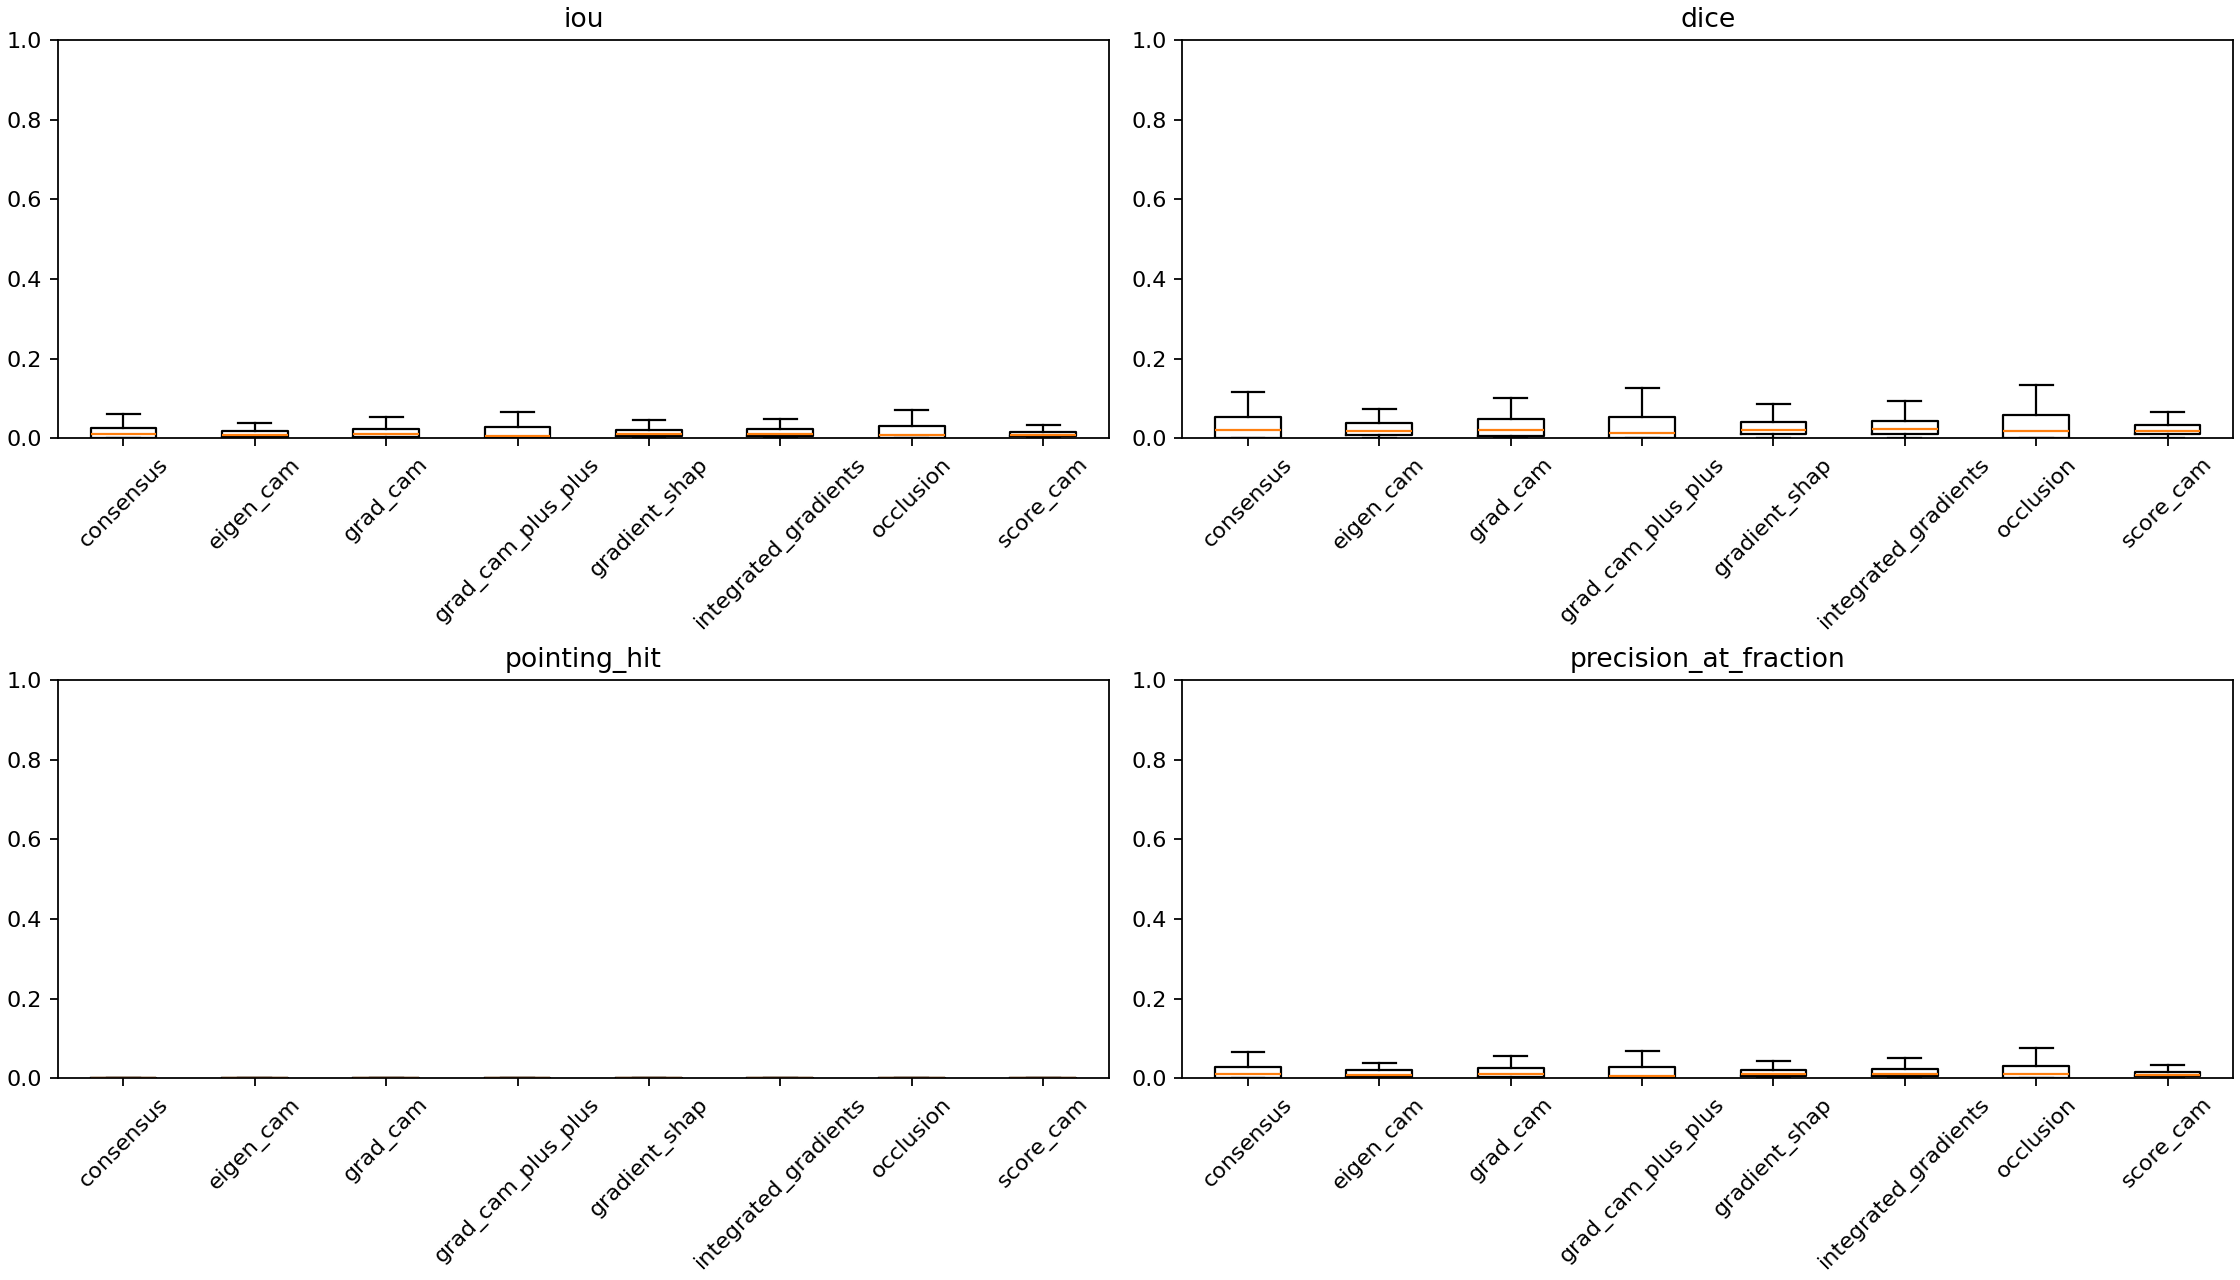
\includegraphics[width=0.85\linewidth,height=0.42\textheight,keepaspectratio]{figures/iter_58_chex_improvement_v3__improvement_experiment_boxplots.png}
	\caption{DenseNet-chex localization metric distributions}
	\label{graph:4-2}
\end{graph}

\begin{graph}[htbp]
	\centering
	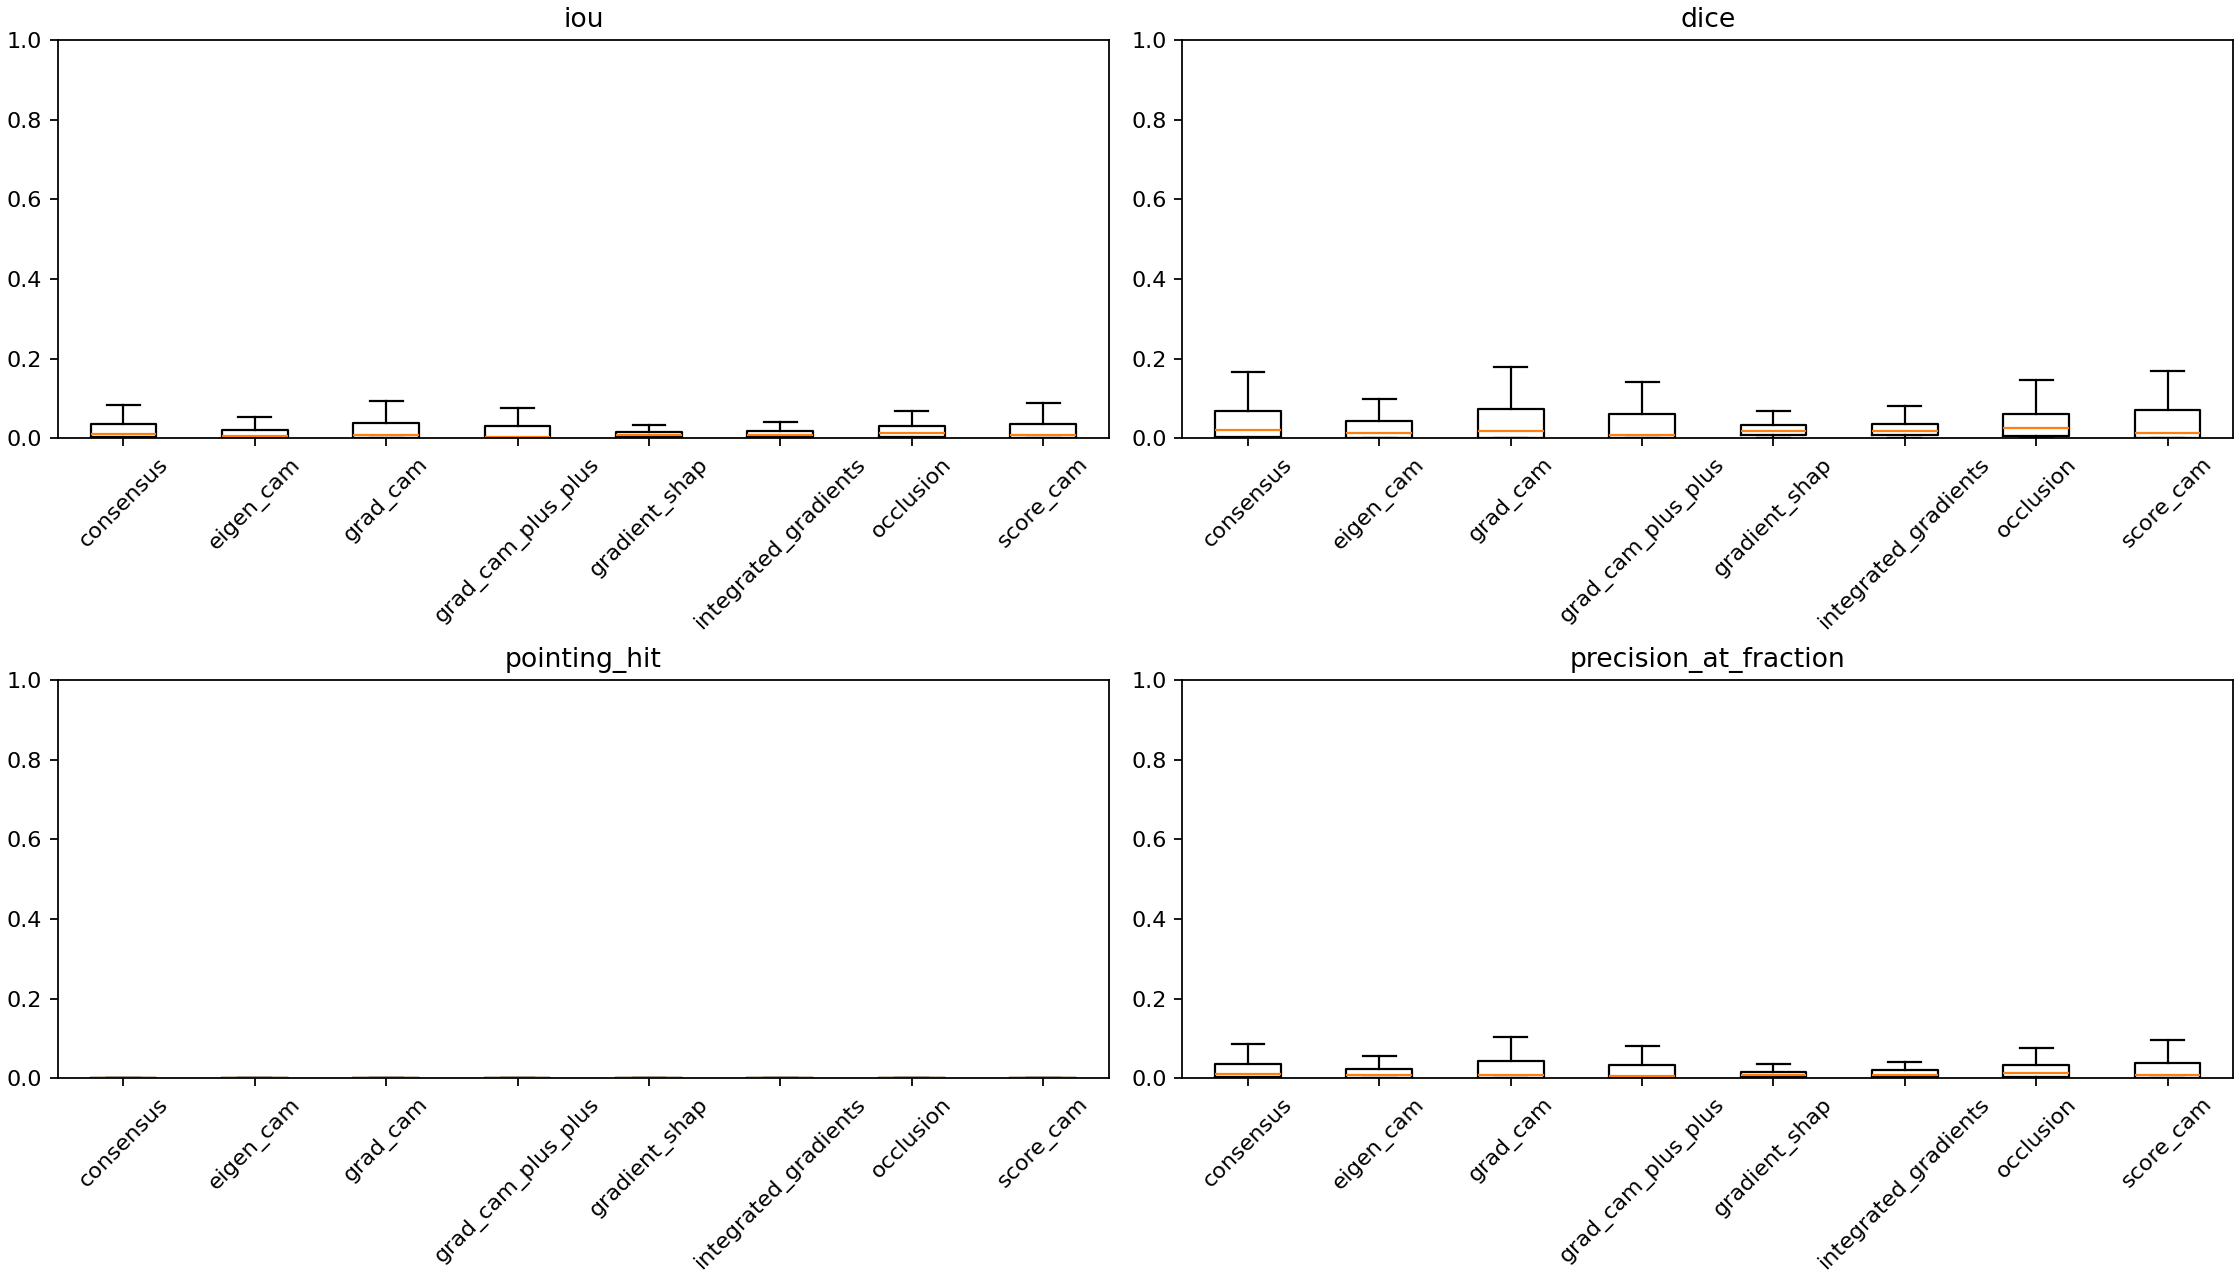
\includegraphics[width=0.85\linewidth,height=0.42\textheight,keepaspectratio]{figures/iter_52_resnet_improvement_v3__improvement_experiment_boxplots.png}
	\caption{ResNet-50 localization metric distributions}
	\label{graph:4-3}
\end{graph}

Faithfulness was evaluated on the final ResNet-50 baseline over the 40
balanced review cases, using deletion and insertion curves with a
normalized black-image baseline, and is reported separately for each
classifier outcome (Graph~\ref{graph:4-6}). All four groups stay within a
narrow band near \texttt{0.\allowbreak 5}: the black baseline itself scores about
\texttt{0.\allowbreak 5} pneumothorax and the models are only weakly confident even
when correct (true-positive probabilities reach only about
\texttt{0.\allowbreak 55--0.\allowbreak 58}), so the available dynamic range is small. Within
that band the curves move in the expected directions but only slightly.
The clearest signal is a modest insertion gain for the CAM-family methods
and Occlusion in the three label-related groups (TP, FP, and FN), where
restoring the top-attributed pixels lifts the probability by roughly
\texttt{0.\allowbreak 05--0.\allowbreak 08}, while Integrated Gradients and
GradientSHAP stay flat; deletion produces only a small monotonic
drop for those same groups, and the true-negative group is essentially
flat in both panels. The reading is that faithfulness separation is weak
for these off-the-shelf attributions, and that the CAM-family maps are
marginally more model-faithful than the pixel-attribution methods, but no
outcome shows strong faithfulness. This is consistent with the weak mask
overlap reported above: a method can move the model probability in the
expected direction while still attributing to non-lesion structure, so
faithfulness to the classifier does not imply clinically correct
localization. Faithfulness was assessed on the co-primary ResNet-50 model
here (consensus and its constituent methods plus Grad-CAM++)
and on the CT pilot in Appendix~\ref{additional-figures}.

\begin{graph}[htbp]
	\centering
	\begin{minipage}{\linewidth}
		\centering
		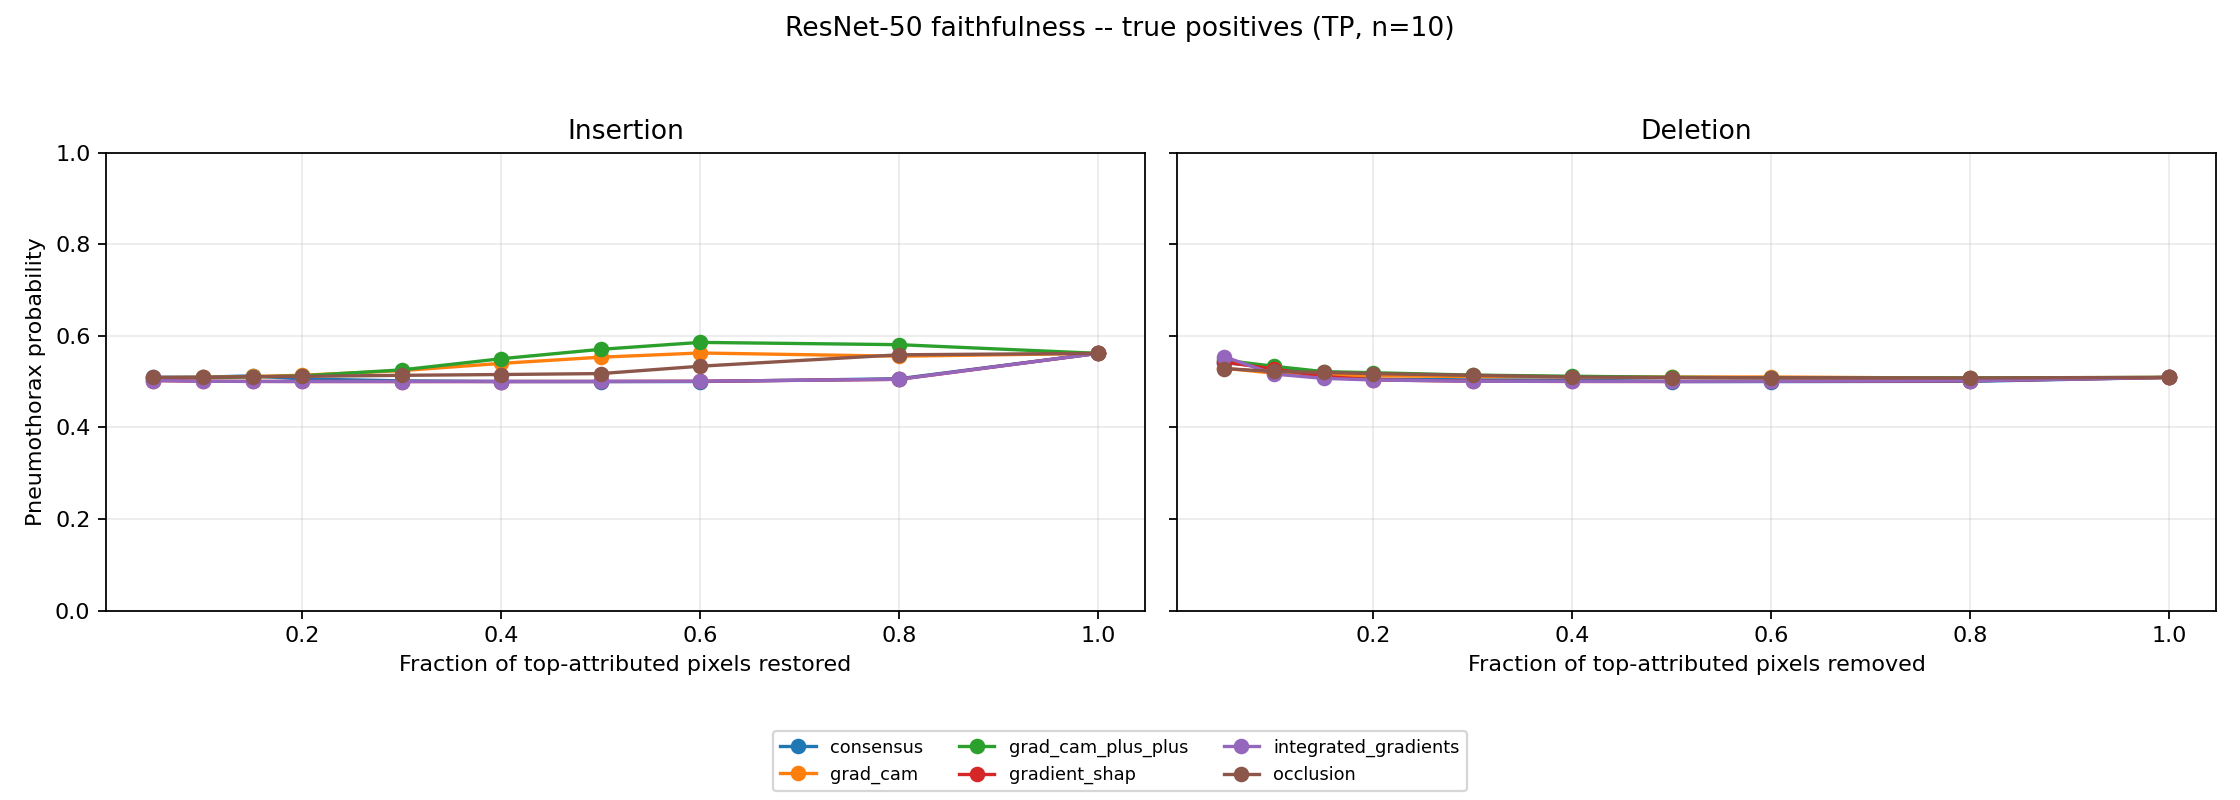
\includegraphics[width=0.92\linewidth,height=0.19\textheight,keepaspectratio]{figures/iter_47_resnet_faithfulness_tp__faithfulness_curves.png}
		\subcaption{True positives (TP)}
	\end{minipage}

	\vspace{0.4em}

	\begin{minipage}{\linewidth}
		\centering
		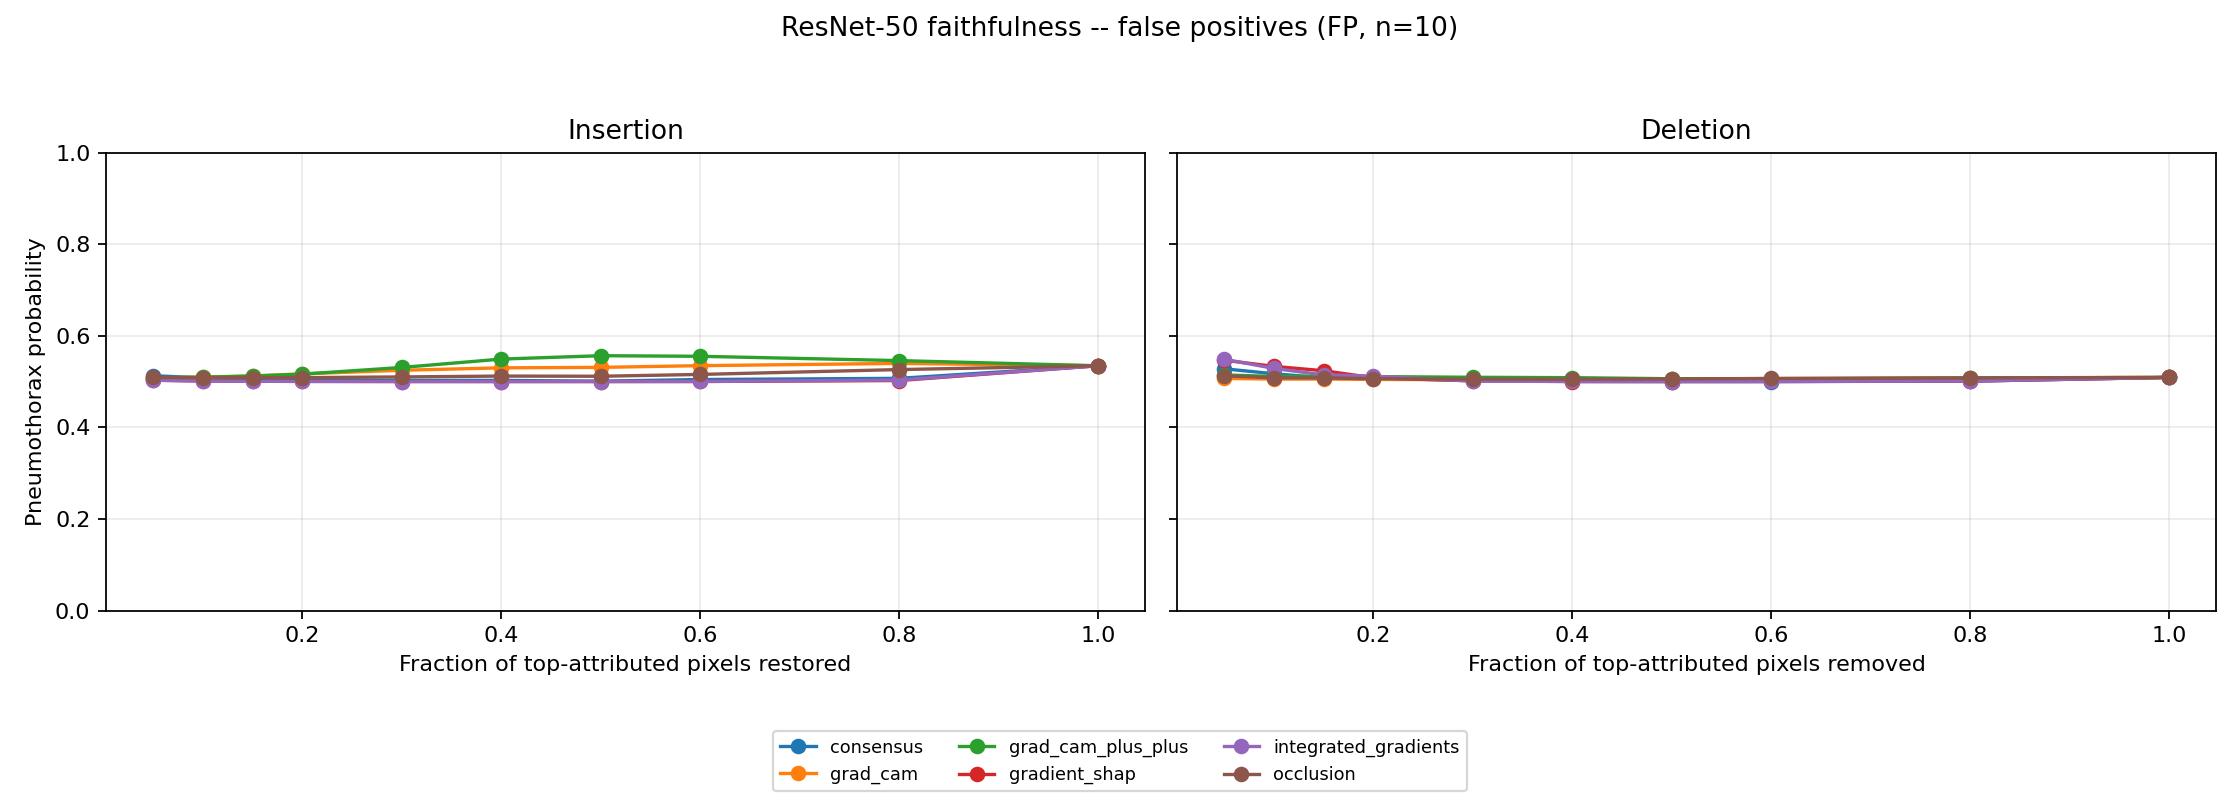
\includegraphics[width=0.92\linewidth,height=0.19\textheight,keepaspectratio]{figures/iter_47_resnet_faithfulness_fp__faithfulness_curves.png}
		\subcaption{False positives (FP)}
	\end{minipage}

	\vspace{0.4em}

	\begin{minipage}{\linewidth}
		\centering
		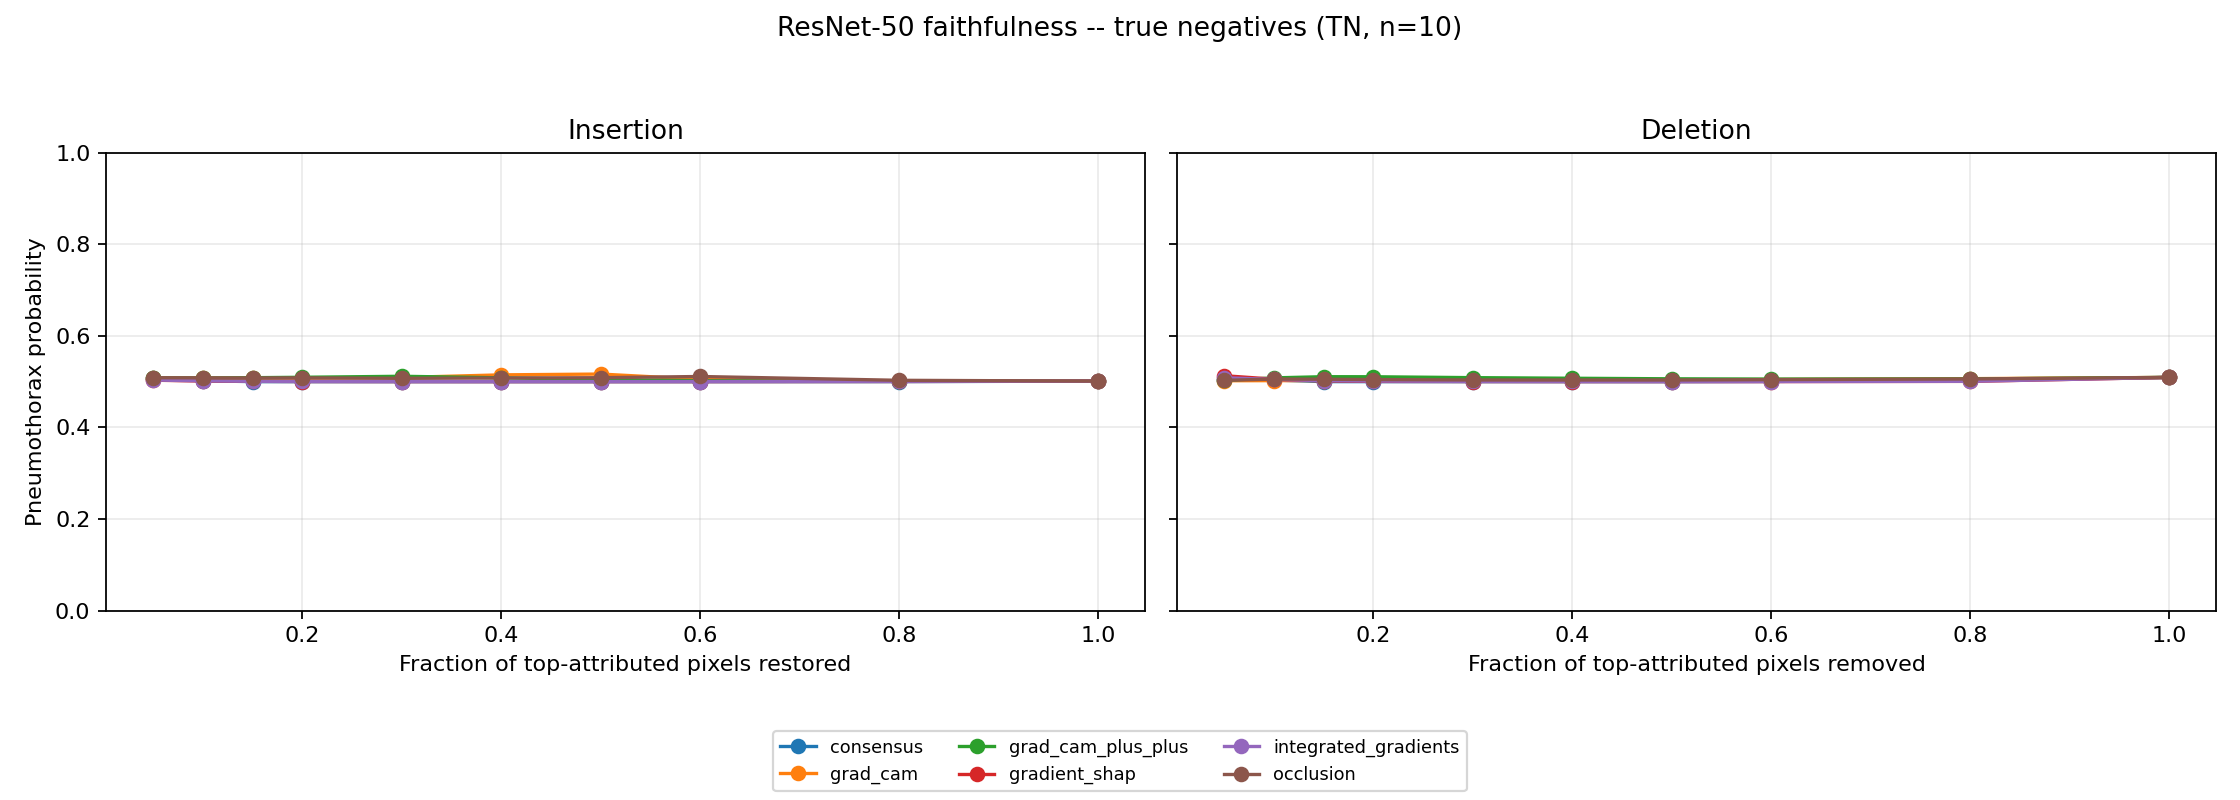
\includegraphics[width=0.92\linewidth,height=0.19\textheight,keepaspectratio]{figures/iter_47_resnet_faithfulness_tn__faithfulness_curves.png}
		\subcaption{True negatives (TN)}
	\end{minipage}

	\vspace{0.4em}

	\begin{minipage}{\linewidth}
		\centering
		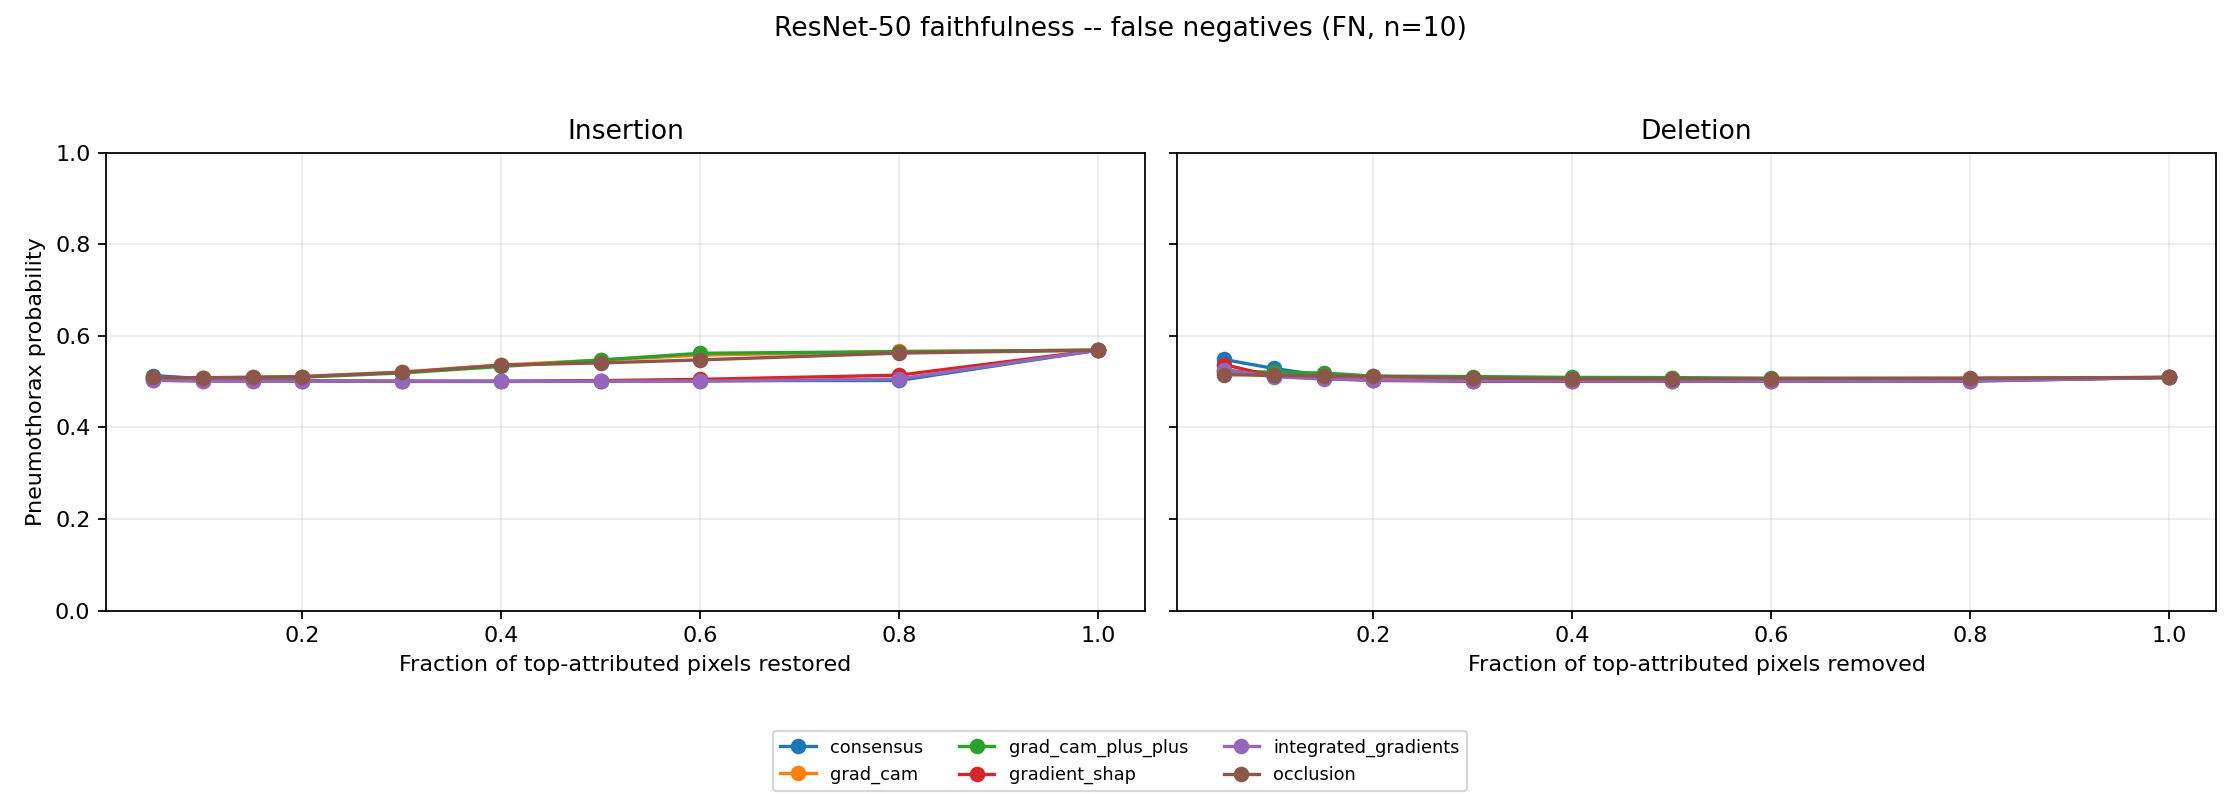
\includegraphics[width=0.92\linewidth,height=0.19\textheight,keepaspectratio]{figures/iter_47_resnet_faithfulness_fn__faithfulness_curves.png}
		\subcaption{False negatives (FN)}
	\end{minipage}
	\caption{Deletion and insertion faithfulness curves for the ResNet-50
		baseline, split by classifier outcome (10 balanced review cases per
		group; positive-view attributions, normalized black-image baseline)}
	\label{graph:4-6}
\end{graph}

\hypertarget{cross-modality-comparison}{%
	\section{Cross-Modality Comparison}\label{cross-modality-comparison}}

The cross-modality result are asymmetric. The CXR
experiments evaluate the frozen four-method consensus across CAM,
input-gradient, and perturbation families. The CT experiment evaluates
an input-space consensus of
Integrated Gradients, GradientSHAP, and
Occlusion, because the convolutional CAM implementation does
not transfer directly to the Vision Transformer checkpoint. 

Table \ref{table:4-3} summarizes the corrected cross-modality consensus reading. The
important negative result is that there was no general trend that
consensus improves localization. DenseNet-chex shows significant overlap
gains mainly over Score-CAM, while stronger aggregate Dice
methods remain competitive or better descriptively. ResNet-50 shows
small significant overlap gains over weaker methods while tying the
strongest CAM methods. CT shows the cleanest consensus benefit, but only
for peak localization (\texttt{Pointing \allowbreak hit}), while broad overlap
metrics remain non-significant.

\begin{longtable}[]{@{}llllll@{}}
	\caption{Cross-modality consensus summary}\tabularnewline
	\toprule
	\begin{minipage}[b]{0.14\columnwidth}\raggedright
		Setting\strut
	\end{minipage} & \begin{minipage}[b]{0.14\columnwidth}\raggedright
		Reference consensus\strut
	\end{minipage} & \begin{minipage}[b]{0.12\columnwidth}\raggedright
		Test set\strut
	\end{minipage} & \begin{minipage}[b]{0.14\columnwidth}\raggedright
		Main significant result\strut
	\end{minipage} & \begin{minipage}[b]{0.16\columnwidth}\raggedright
		Aggregate consensus metrics\strut
	\end{minipage} & \begin{minipage}[b]{0.14\columnwidth}\raggedright
		Thesis interpretation\strut
	\end{minipage}\tabularnewline
	\midrule
	\endfirsthead
	\toprule
	\begin{minipage}[b]{0.14\columnwidth}\raggedright
		Setting\strut
	\end{minipage} & \begin{minipage}[b]{0.14\columnwidth}\raggedright
		Reference consensus\strut
	\end{minipage} & \begin{minipage}[b]{0.12\columnwidth}\raggedright
		Test set\strut
	\end{minipage} & \begin{minipage}[b]{0.14\columnwidth}\raggedright
		Main significant result\strut
	\end{minipage} & \begin{minipage}[b]{0.16\columnwidth}\raggedright
		Aggregate consensus metrics\strut
	\end{minipage} & \begin{minipage}[b]{0.14\columnwidth}\raggedright
		Thesis interpretation\strut
	\end{minipage}\tabularnewline
	\midrule
	\endhead
	\begin{minipage}[t]{0.14\columnwidth}\raggedright
		CXR DenseNet-chex\strut
	\end{minipage} & \begin{minipage}[t]{0.14\columnwidth}\raggedright
		frozen four-method CXR consensus\strut
	\end{minipage} & \begin{minipage}[t]{0.12\columnwidth}\raggedright
		\texttt{200} SIIM test positives\strut
	\end{minipage} & \begin{minipage}[t]{0.14\columnwidth}\raggedright
		Dice/ IoU/ Precision higher than Score-CAM; Pointing hit varies, 
		however, does not impact the median\strut
	\end{minipage} & \begin{minipage}[t]{0.16\columnwidth}\raggedright
		IoU \texttt{0.\allowbreak 0203}, 
		
		Dice \texttt{0.\allowbreak 0383}, 
		
		pointing \texttt{0.\allowbreak 050},
		
		precision \texttt{0.\allowbreak 0213}\strut
	\end{minipage} & \begin{minipage}[t]{0.14\columnwidth}\raggedright
		consensus is competitive but not best by aggregate Dice; not universally
		superior\strut
	\end{minipage}\tabularnewline
	\begin{minipage}[t]{0.14\columnwidth}\raggedright
		CXR ResNet-50\strut
	\end{minipage} & \begin{minipage}[t]{0.14\columnwidth}\raggedright
		frozen four-method CXR consensus\strut
	\end{minipage} & \begin{minipage}[t]{0.12\columnwidth}\raggedright
		\texttt{200} SIIM test positives\strut
	\end{minipage} & \begin{minipage}[t]{0.14\columnwidth}\raggedright
		Dice/ IoU/ precision higher than five weaker methods; not significant vs
		Grad-CAM or Score-CAM\strut
	\end{minipage} & \begin{minipage}[t]{0.16\columnwidth}\raggedright
		IoU \texttt{0.\allowbreak 0265}, 
		
		Dice \texttt{0.\allowbreak 0488}, 
		
		pointing \texttt{0.\allowbreak 010},
		
		precision \texttt{0.\allowbreak 0289}\strut
	\end{minipage} & \begin{minipage}[t]{0.14\columnwidth}\raggedright
		consensus stabilizes weak/noisy methods but remains comparable to the
		best CAM alternatives\strut
	\end{minipage}\tabularnewline
	\begin{minipage}[t]{0.14\columnwidth}\raggedright
		CT DifeiT ViT\strut
	\end{minipage} & \begin{minipage}[t]{0.14\columnwidth}\raggedright
		three-method input-space consensus\strut
	\end{minipage} & \begin{minipage}[t]{0.12\columnwidth}\raggedright
		\texttt{105} PhysioNet CT positive slices\strut
	\end{minipage} & \begin{minipage}[t]{0.14\columnwidth}\raggedright
		pointing-hit significantly higher than Integrated Gradients, GradientSHAP, and Occlusion;
		overlap metrics non-significant\strut
	\end{minipage} & \begin{minipage}[t]{0.16\columnwidth}\raggedright
		IoU \texttt{0.\allowbreak 0411}, 
		
		Dice \texttt{0.\allowbreak 0754}, 
		
		pointing \texttt{0.\allowbreak 343},
		
		precision \texttt{0.\allowbreak 0458}\strut
	\end{minipage} & \begin{minipage}[t]{0.14\columnwidth}\raggedright
		strongest consensus signal is peak localization on CT, not broad
		overlap\strut
	\end{minipage}\tabularnewline
	\bottomrule
	\label{table:4-3}
\end{longtable}

The CT finding should be reported with four caveats. First, the CT
calibration selected fraction \texttt{0.\allowbreak 05} for all methods, which is
the floor of the sweep and suggests that smaller fractions may be
relevant for tiny hemorrhage masks. Second, \texttt{pointing \allowbreak hit} is
binary per case, so the proper interpretation combines per-method rates,
win/tie/loss counts, and the paired rank test; median paired differences
alone are not sufficiently informative. Third, the CT experiment uses one classifier and
one dataset only. Fourth, CAM-family transformer explanations were excluded
because adopting transformer-specific CAM or attention methods
would introduce a different implementation path from the CXR
convolutional code. The CT pilot localization metric distributions are
shown in Graph~\ref{graph:4-4}.

\begin{graph}[htbp]
	\centering
	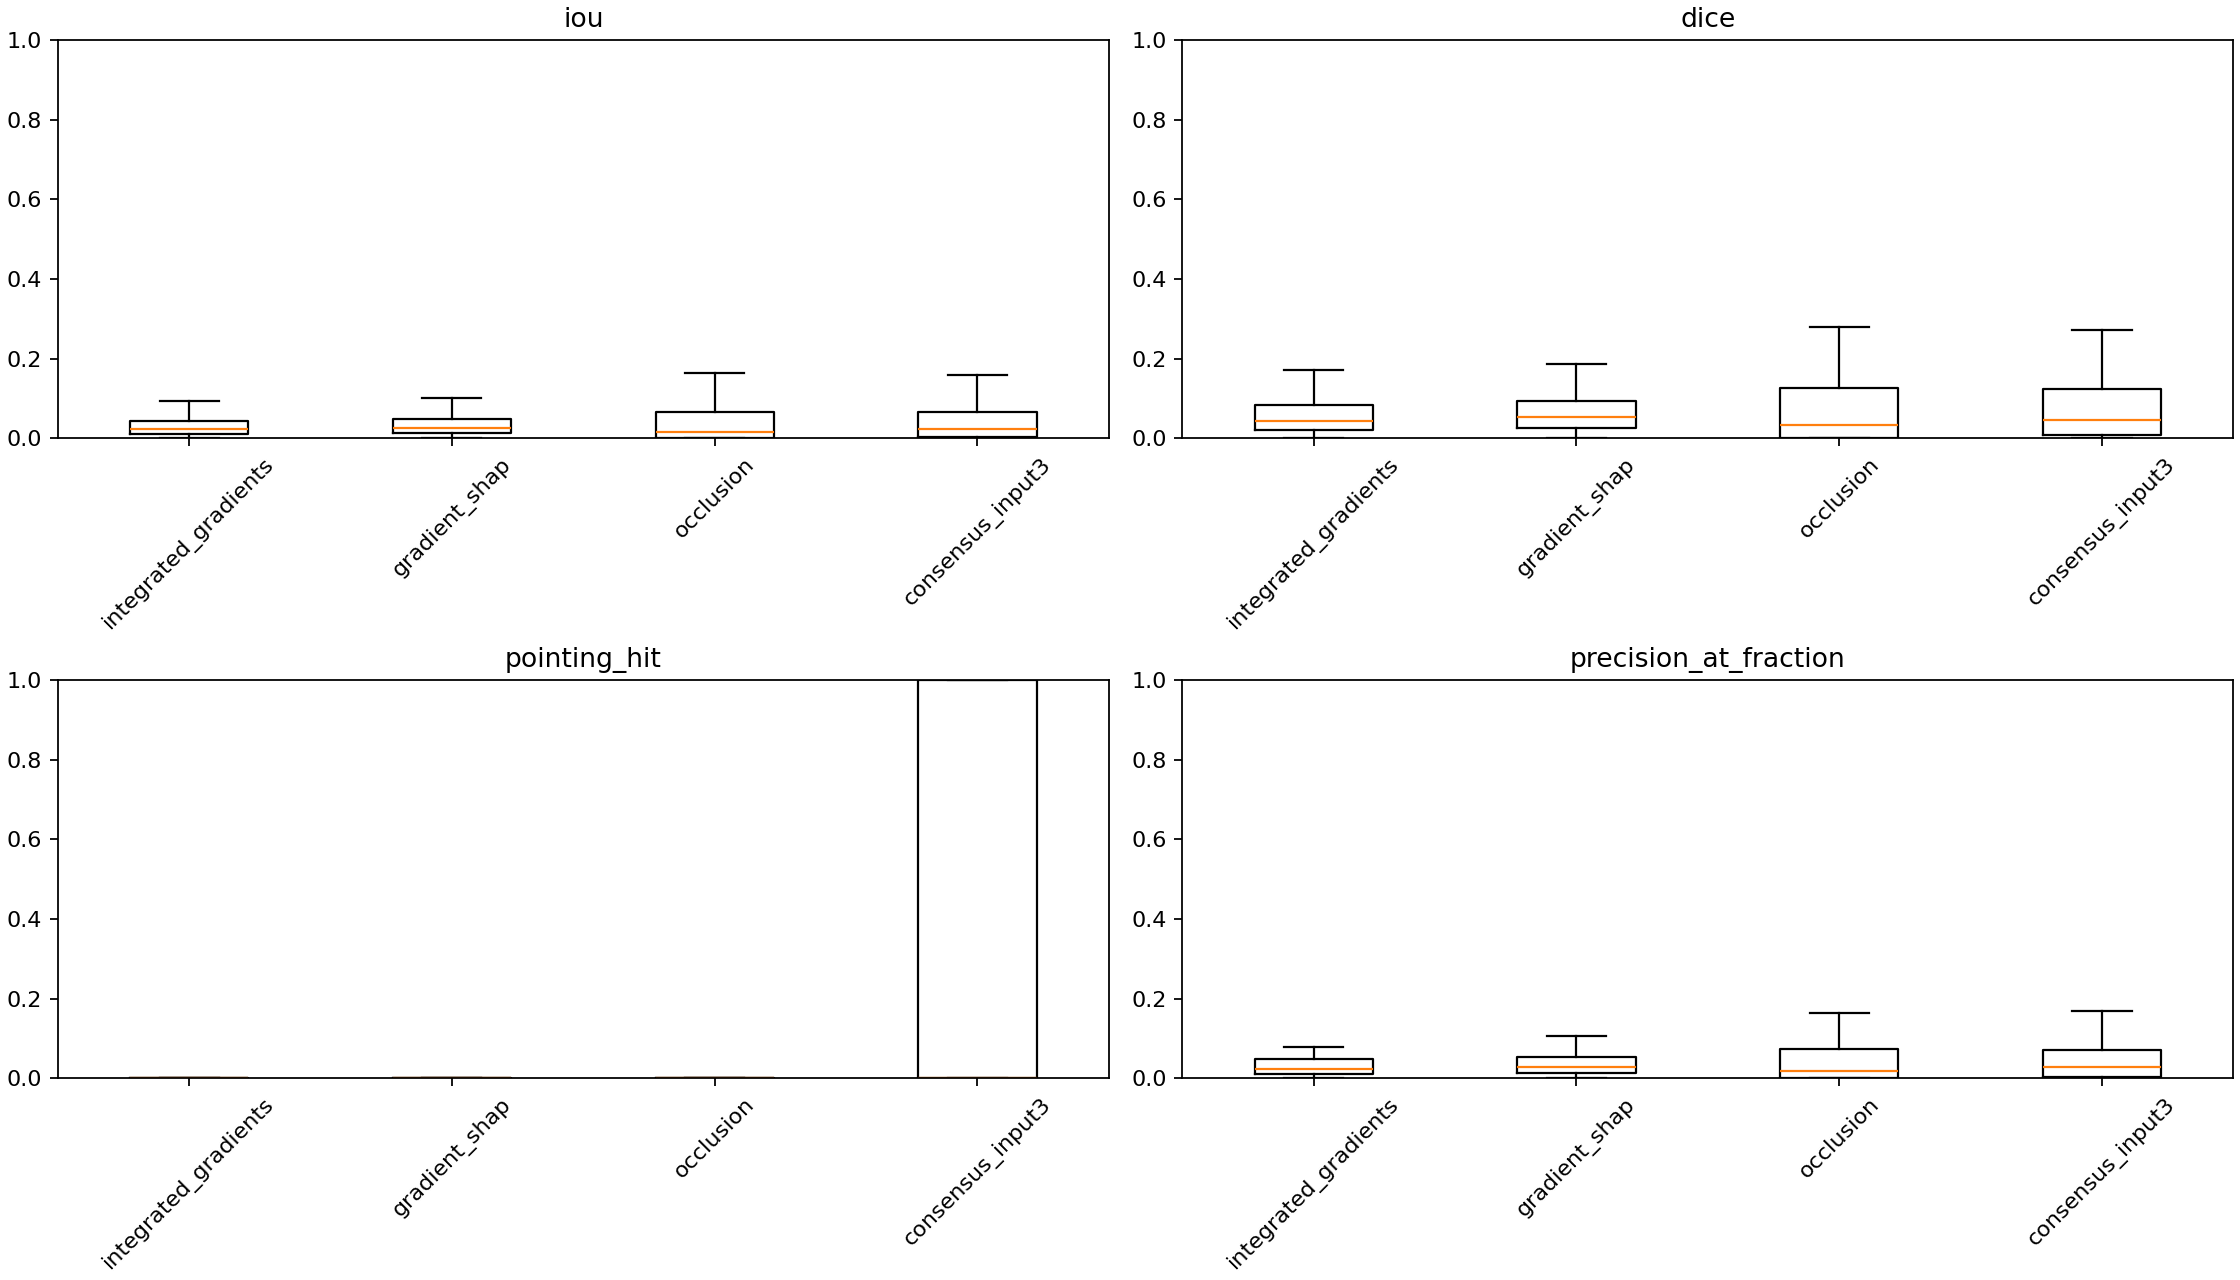
\includegraphics[width=0.85\linewidth,height=0.42\textheight,keepaspectratio]{figures/iter_54_ct_improvement_test__ct_improvement_experiment_boxplots.png}
	\caption{CT pilot localization metric distributions}
	\label{graph:4-4}
\end{graph}

\hypertarget{radiologist-assessment-and-failure-taxonomy}{%
	\section{Radiologist Assessment and Failure
		Taxonomy}\label{radiologist-assessment-and-failure-taxonomy}}

This section combines the automatic metrics with the structured balanced
40-case ResNet review. Alongside the numerical distributions reported
below, it presents a representative visual example
(Figure~\ref{figure:4-1}) that connects the
counts to direct localization, indirect clinically related evidence,
device/tube confusion, high-contrast non-lesion evidence, and
clinically misleading maps.

\begin{figure}[htbp]
	\centering
	
\includegraphics[width=0.316\linewidth,height=0.32\textheight,keepaspectratio]{figures/iter_48_resnet_review_workbook_balanced40_smoothed_faithfulness__review__assets__case_31__101_test_1_.png}%
	\hfill
	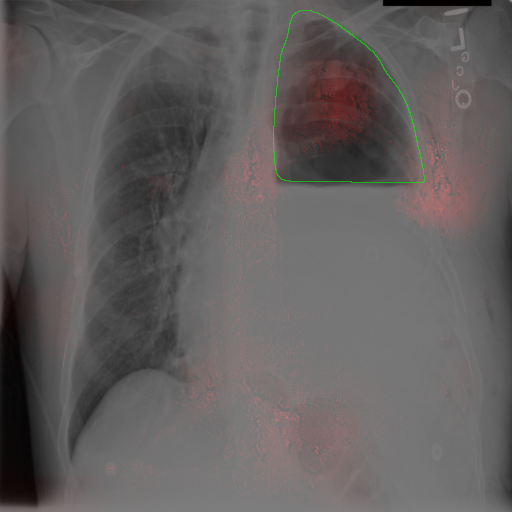
\includegraphics[width=0.316\linewidth,height=0.32\textheight,keepaspectratio]{figures/iter_48_resnet_review_workbook_balanced40_smoothed_faithfulness__review__assets__case_31__101_test_1__consensus_continuous_heatmap.png}%
	\hfill
	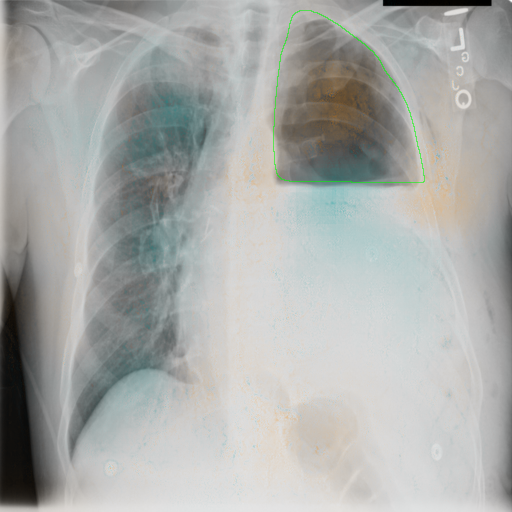
\includegraphics[width=0.316\linewidth,height=0.32\textheight,keepaspectratio]{figures/iter_48_resnet_review_workbook_balanced40_smoothed_faithfulness__review__assets__case_31__101_test_1__consensus_signed_continuous_heatmap.png}%
	\vfill
	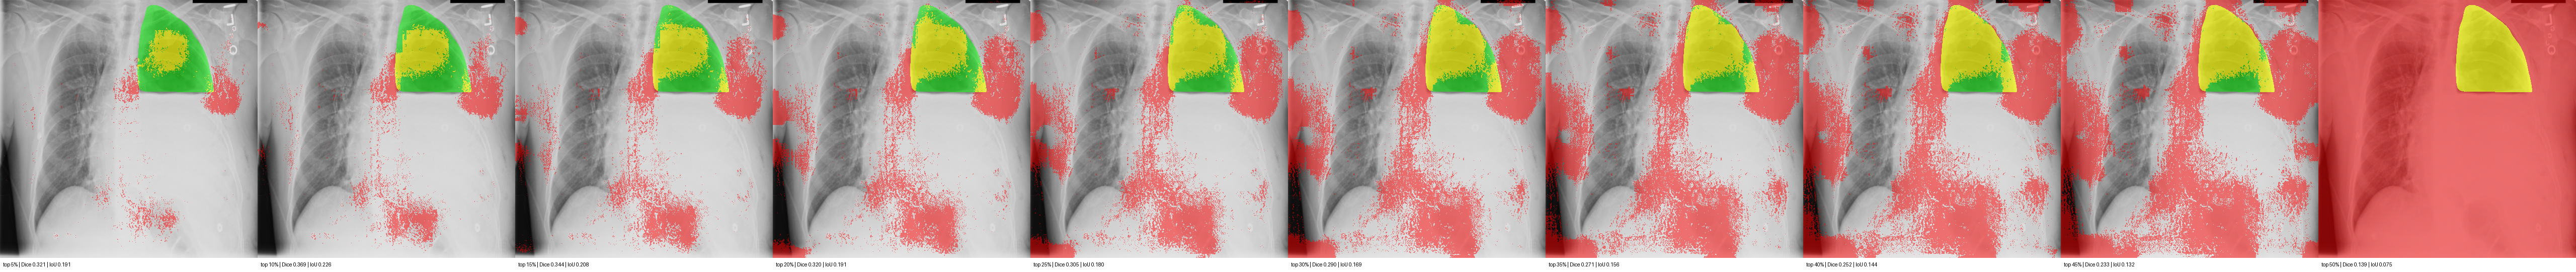
\includegraphics[width=0.99\linewidth,height=0.32\textheight,keepaspectratio]{figures/iter_48_resnet_review_workbook_balanced40_smoothed_faithfulness__review__assets__case_31__101_test_1__consensus_threshold_sweep_panel.png}%
	\caption{Representative review-workbook case for explanation visual inspection (false-negative outcome with correct lesion localization: the classifier scored the case below threshold while the explanation still localized the pneumothorax)}
	\label{figure:4-1}
\end{figure}

Key interpretation points from the balanced 40-case ResNet review
(scored 2026-05-25) are summarized below. 
\begin{itemize}
\item Review score distribution
(\texttt{n=40}, with 10 cases per
\texttt{tp}/\texttt{fp}/\texttt{tn}/\texttt{fn} outcome): localization
was \texttt{correct} in 11/40 cases, \texttt{partial} in 15/40, and
\texttt{incorrect} in 14/40. Usefulness was \texttt{useful} in 12/40,
\texttt{potentially \allowbreak useful} in 13/40, \texttt{misleading} in 14/40, and
\texttt{not \allowbreak useful} in 1/40. The split between useful + potentially
useful (25/40) and misleading + not useful (15/40) supports the idea that
 many maps carry some interpretable signal, but
clinically misleading or poorly localized explanations remain common.
\item
Failure taxonomy counts: \texttt{correct} 10/40, \texttt{partial} 8/40,
\texttt{non \allowbreak pathological \allowbreak high \allowbreak contrast} 13/40,
\texttt{clinically \allowbreak misleading} 7/40, and
\texttt{devices \allowbreak or text \allowbreak artifacts} 2/40. The two remaining schema
categories, \texttt{anatomically \allowbreak related} and
\texttt{diffuse \allowbreak non \allowbreak specific}, received no primary assignments in this
balanced set (0/40 each); clinically adjacent indirect evidence is instead
captured by the separate qualitative flags reported below. The dominant
failure mode at
this stage of the off-the-shelf TorchXRayVision baseline is attention on
non-pathological high-contrast structures (bones, rib edges, lung apex)
rather than on device/text artifacts.
\item Devices/tubes were relevant in 19/40 cases,
indirect evidence in 8/40, method disagreement in 8/40, weak pixel
attribution in 4/40, subcutaneous emphysema in 4/40, and a mask-quality
issues in 3/40. The high devices/tubes flag rate is a structural
confounder of the off-the-shelf classifier on SIIM pneumothorax: devices
can be present in both positive and negative cases, and the classifier's 
evidence frequently refers to them instead of pneumothorax-specific
findings.
\item Device/tube and subcutaneous-emphysema
findings should not be grouped together as generic artifacts. 
Tubes are treatment related findings and may have better correlation with actual pneumothorax,
while other devices, ECG wires and subcutaneous emphysema separate findings, whilst the emphysema 
itself can be an extremely strong confusion factor, if it overlaps the region, where pneumothorax is expected. 
\item The 40-case balanced review supports using
\texttt{usefulness \allowbreak score} separately from \texttt{localization \allowbreak score}.
Low-overlap maps can still be useful for auditing model failure or
identifying clinically adjacent evidence; conversely, a visually
plausible map can be misleading if it emphasizes non-lesion regions.
\item
In the review workbook and figures it is important to remember that heatmaps visualize
model attribution toward the selected pneumothorax output and should not
be interpreted as anatomical segmentations.
\item Exploratory score-metric
correlations on the balanced 40-case set the strongest absolute
Spearman associations are about
\texttt{\textbar{}rho\textbar{}\ \textless{}=\ 0.\allowbreak 42}. 
This means that there was no metric in this test that automatically 
captured the clinical usefulness. 
\end{itemize}

Chart \ref{chart:4-2} visualizes the balanced 40-case review score
distribution as review-score counts.

\begin{chart}[htbp]
	\centering
	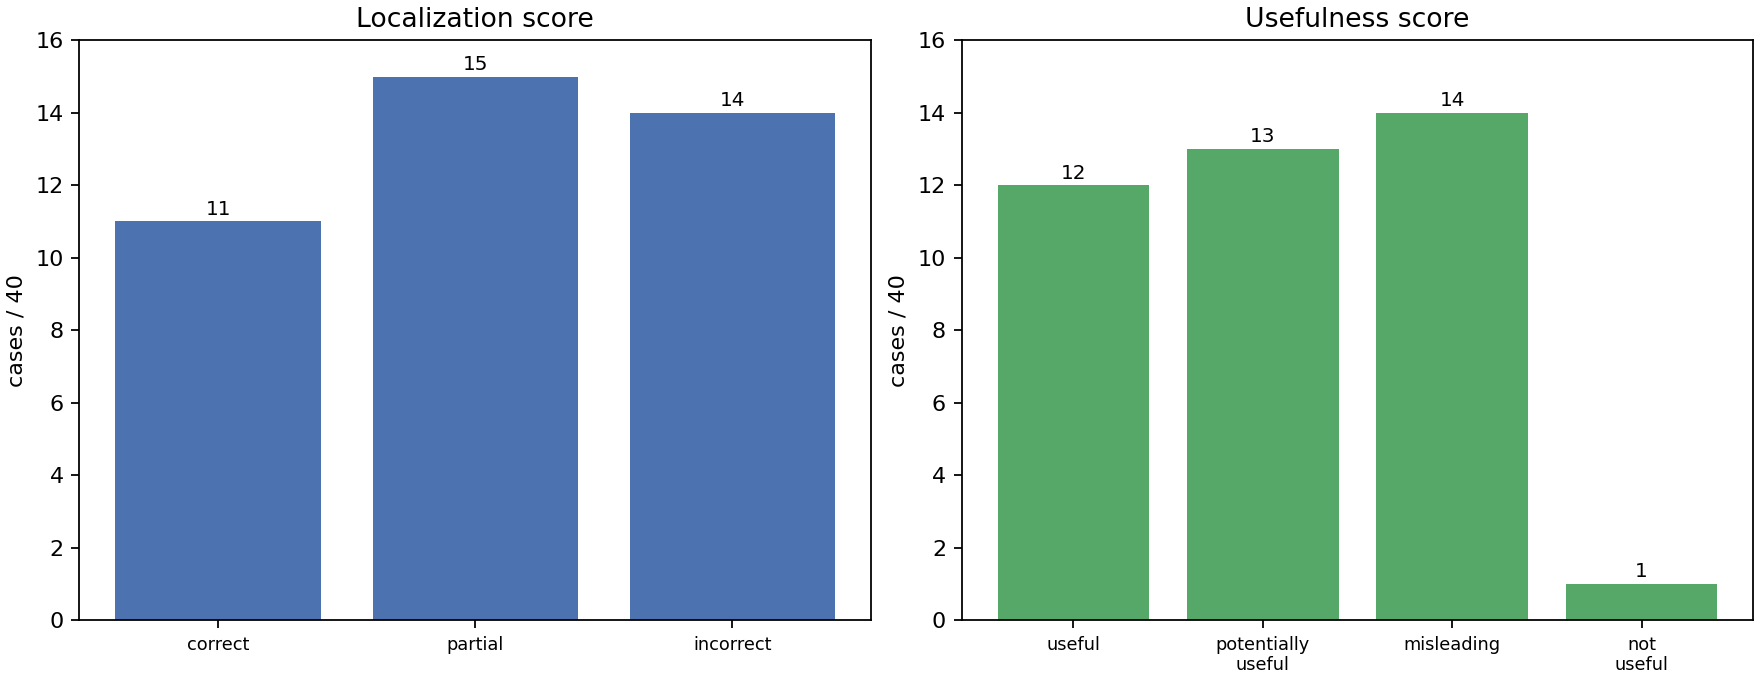
\includegraphics[width=0.85\linewidth,height=0.42\textheight,keepaspectratio]{figures/iter_61_thesis_charts__chart_4_2_review_scores.png}
	\caption{Balanced 40-case review score distribution (localization and usefulness)}
	\label{chart:4-2}
\end{chart}



\begin{longtable}[]{@{}lll@{}}
	\caption{Balanced 40-case radiologist review score
		distribution}\tabularnewline
	\toprule
	\begin{minipage}[b]{0.20\columnwidth}\raggedright
		Review dimension\strut
	\end{minipage} & \begin{minipage}[b]{0.20\columnwidth}\raggedright
		Category\strut
	\end{minipage} & \begin{minipage}[b]{0.40\columnwidth}\raggedright
		Interpretation\strut
	\end{minipage}\tabularnewline
	\midrule
	\endfirsthead
	\toprule
	\begin{minipage}[b]{0.20\columnwidth}\raggedright
		Review dimension\strut
	\end{minipage} & \begin{minipage}[b]{0.20\columnwidth}\raggedright
		Category\strut
	\end{minipage} & \begin{minipage}[b]{0.40\columnwidth}\raggedright
		Interpretation\strut
	\end{minipage}\tabularnewline
	\midrule
	\endhead
	\begin{minipage}[t]{0.20\columnwidth}\raggedright
		Localization\strut
	\end{minipage} & \begin{minipage}[t]{0.20\columnwidth}\raggedright
		\texttt{correct}\strut
	\end{minipage} & \begin{minipage}[t]{0.40\columnwidth}\raggedright
		clear lesion-aligned evidence in a minority of cases\strut
	\end{minipage}\tabularnewline
	\begin{minipage}[t]{0.20\columnwidth}\raggedright
		Localization\strut
	\end{minipage} & \begin{minipage}[t]{0.20\columnwidth}\raggedright
		\texttt{partial}\strut
	\end{minipage} & \begin{minipage}[t]{0.40\columnwidth}\raggedright
		some plausible evidence present, but incomplete or indirect\strut
	\end{minipage}\tabularnewline
	\begin{minipage}[t]{0.20\columnwidth}\raggedright
		Localization\strut
	\end{minipage} & \begin{minipage}[t]{0.20\columnwidth}\raggedright
		\texttt{incorrect}\strut
	\end{minipage} & \begin{minipage}[t]{0.40\columnwidth}\raggedright
		notably clinically weak or mislocalized explanations\strut
	\end{minipage}\tabularnewline
	\begin{minipage}[t]{0.20\columnwidth}\raggedright
		Usefulness\strut
	\end{minipage} & \begin{minipage}[t]{0.20\columnwidth}\raggedright
		\texttt{useful}\strut
	\end{minipage} & \begin{minipage}[t]{0.40\columnwidth}\raggedright
		directly helpful for model-audit interpretation\strut
	\end{minipage}\tabularnewline
	\begin{minipage}[t]{0.20\columnwidth}\raggedright
		Usefulness\strut
	\end{minipage} & \begin{minipage}[t]{0.20\columnwidth}\raggedright
		\texttt{potentially \allowbreak useful}\strut
	\end{minipage} & \begin{minipage}[t]{0.40\columnwidth}\raggedright
		informative but requiring caution and context\strut
	\end{minipage}\tabularnewline
	\begin{minipage}[t]{0.20\columnwidth}\raggedright
		Usefulness\strut
	\end{minipage} & \begin{minipage}[t]{0.20\columnwidth}\raggedright
		\texttt{misleading}\strut
	\end{minipage} & \begin{minipage}[t]{0.40\columnwidth}\raggedright
		clinically misleading evidence remains common\strut
	\end{minipage}\tabularnewline
	\begin{minipage}[t]{0.20\columnwidth}\raggedright
		Usefulness\strut
	\end{minipage} & \begin{minipage}[t]{0.20\columnwidth}\raggedright
		\texttt{not \allowbreak useful}\strut
	\end{minipage} & \begin{minipage}[t]{0.40\columnwidth}\raggedright
		no practically useful signal in the scored view\strut
	\end{minipage}\tabularnewline
	\bottomrule
	\label{table:4-4}
\end{longtable}

Table \ref{table:4-5} summarizes the failure taxonomy for the same review set.

Chart \ref{chart:4-3} visualizes failure-taxonomy counts
alongside the qualitative review flags.

\begin{chart}[htbp]
	\centering
	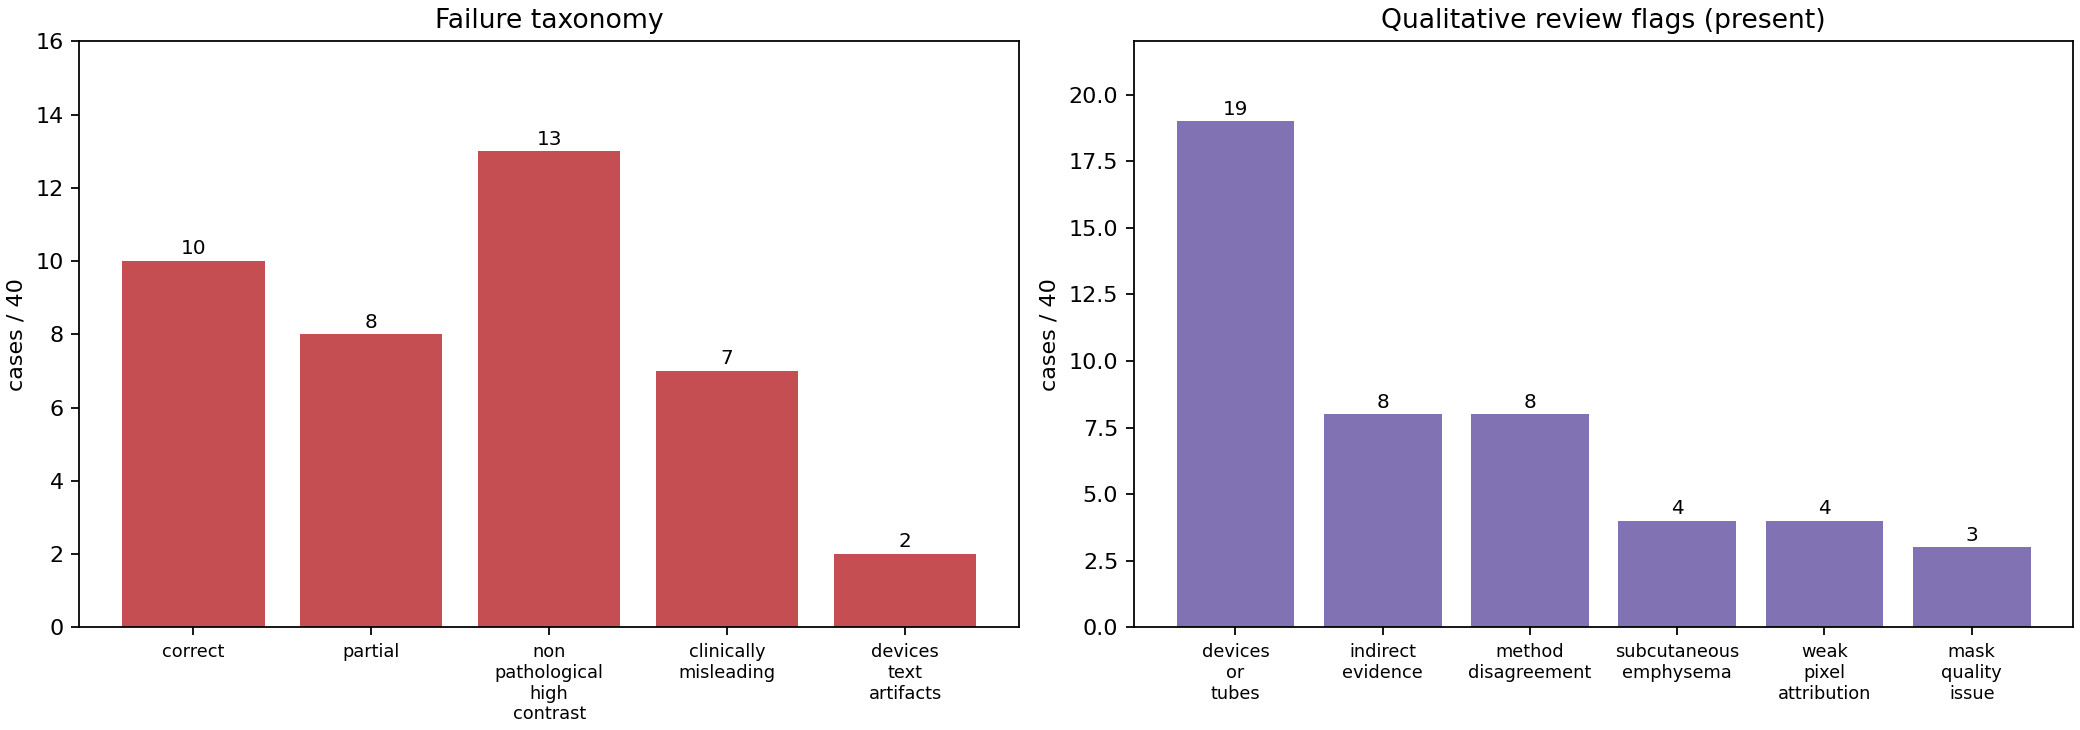
\includegraphics[width=0.85\linewidth,height=0.42\textheight,keepaspectratio]{figures/iter_61_thesis_charts__chart_4_3_failure_taxonomy.png}
	\caption{Balanced 40-case review failure taxonomy and qualitative flags}
	\label{chart:4-3}
\end{chart}

\begin{longtable}[]{@{}ll@{}}
	\caption{Balanced 40-case review failure taxonomy}\tabularnewline
	\toprule
	\begin{minipage}[b]{0.3\columnwidth}\raggedright
		Failure category\strut
	\end{minipage} & \begin{minipage}[b]{0.65\columnwidth}\raggedright
		Interpretation\strut
	\end{minipage}\tabularnewline
	\midrule
	\endfirsthead
	\toprule
	\begin{minipage}[b]{0.3\columnwidth}\raggedright
		Failure category\strut
	\end{minipage} & \begin{minipage}[b]{0.65\columnwidth}\raggedright
		Interpretation\strut
	\end{minipage}\tabularnewline
	\midrule
	\endhead
	\begin{minipage}[t]{0.3\columnwidth}\raggedright
		\texttt{correct}\strut
	\end{minipage} & \begin{minipage}[t]{0.65\columnwidth}\raggedright
		explanation pattern judged clinically aligned\strut
	\end{minipage}\tabularnewline
	\begin{minipage}[t]{0.3\columnwidth}\raggedright
		\texttt{partial}\strut
	\end{minipage} & \begin{minipage}[t]{0.65\columnwidth}\raggedright
		partly aligned or incomplete explanation\strut
	\end{minipage}\tabularnewline
	\begin{minipage}[t]{0.3\columnwidth}\raggedright
		\texttt{non \allowbreak pathological \allowbreak high \allowbreak contrast}\strut
	\end{minipage} & \begin{minipage}[t]{0.65\columnwidth}\raggedright
		dominant failure mode; model evidence often follows high-contrast
		structures rather than pneumothorax mask\strut
	\end{minipage}\tabularnewline
	\begin{minipage}[t]{0.3\columnwidth}\raggedright
		\texttt{clinically \allowbreak misleading}\strut
	\end{minipage} & \begin{minipage}[t]{0.65\columnwidth}\raggedright
		explanation emphasizes regions that could mislead clinical
		interpretation\strut
	\end{minipage}\tabularnewline
	\begin{minipage}[t]{0.3\columnwidth}\raggedright
		\texttt{devices \allowbreak text \allowbreak artifacts}\strut
	\end{minipage} & \begin{minipage}[t]{0.65\columnwidth}\raggedright
		explicit device/text artifact category; separate from clinically related
		tubes or subcutaneous emphysema notes\strut
	\end{minipage}\tabularnewline
	\begin{minipage}[t]{0.3\columnwidth}\raggedright
		\texttt{anatomically \allowbreak related}\strut
	\end{minipage} & \begin{minipage}[t]{0.65\columnwidth}\raggedright
		schema category for indirect, clinically adjacent evidence; no primary
		assignments in this balanced set (0/40)\strut
	\end{minipage}\tabularnewline
	\begin{minipage}[t]{0.3\columnwidth}\raggedright
		\texttt{diffuse \allowbreak non \allowbreak specific}\strut
	\end{minipage} & \begin{minipage}[t]{0.65\columnwidth}\raggedright
		schema category for spatially diffuse, non-specific maps; no primary
		assignments in this balanced set (0/40)\strut
	\end{minipage}\tabularnewline
	\bottomrule
	\label{table:4-5}
\end{longtable}

\hypertarget{explanation-improvement-experiment}{%
	\section{Explanation Improvement
		Experiment}\label{explanation-improvement-experiment}}

The explanation-improvement experiment evaluated whether the
frozen four-method consensus improves positive-lesion localization over
individual methods on positive CXR test cases. The
selected-baseline run used train-split top-fraction calibration only.

Each run produced \texttt{1,\allowbreak 600} per-case metric rows (\texttt{200}
cases x \texttt{8} positive-view methods), paired consensus-vs-method
Wilcoxon signed-rank tests, Holm-Bonferroni adjusted p-values, bootstrap
confidence intervals, and aggregate plots. Table \ref{table:4-6} reports the
Dice-focused paired comparison because out of Dice, IoU, pointing hit and \texttt{P@F}, the former is the most interpretable overlap summary for selected attribution regions. 

Exploratory
cross-case pattern analysis found moderately high visual cosine
similarity for Integrated Gradients/GradientSHAP maps across the 10 review cases
(\texttt{mean} roughly \texttt{0.\allowbreak 53-\allowbreak 0.\allowbreak 55} across positive, negative,
magnitude, and signed views). Higher cross-case similarity tended to
associate with lower localization score in this small sample, with the
strongest observed Spearman around \texttt{rho=-\allowbreak 0.\allowbreak 54} on \texttt{n=10}
for magnitude views. This in turn provides evidence that 
pixel-level methods may sometimes show case-invariant or
preprocessing-driven patterns, so qualitative review should check
whether maps are case-specific. The per-method paired
consensus-versus-individual localization differences are shown in
Graph~\ref{graph:4-5}.

\begin{graph}[htbp]
	\centering
	
	% --- Row 1 ---
	\begin{minipage}{\linewidth}
		\centering
		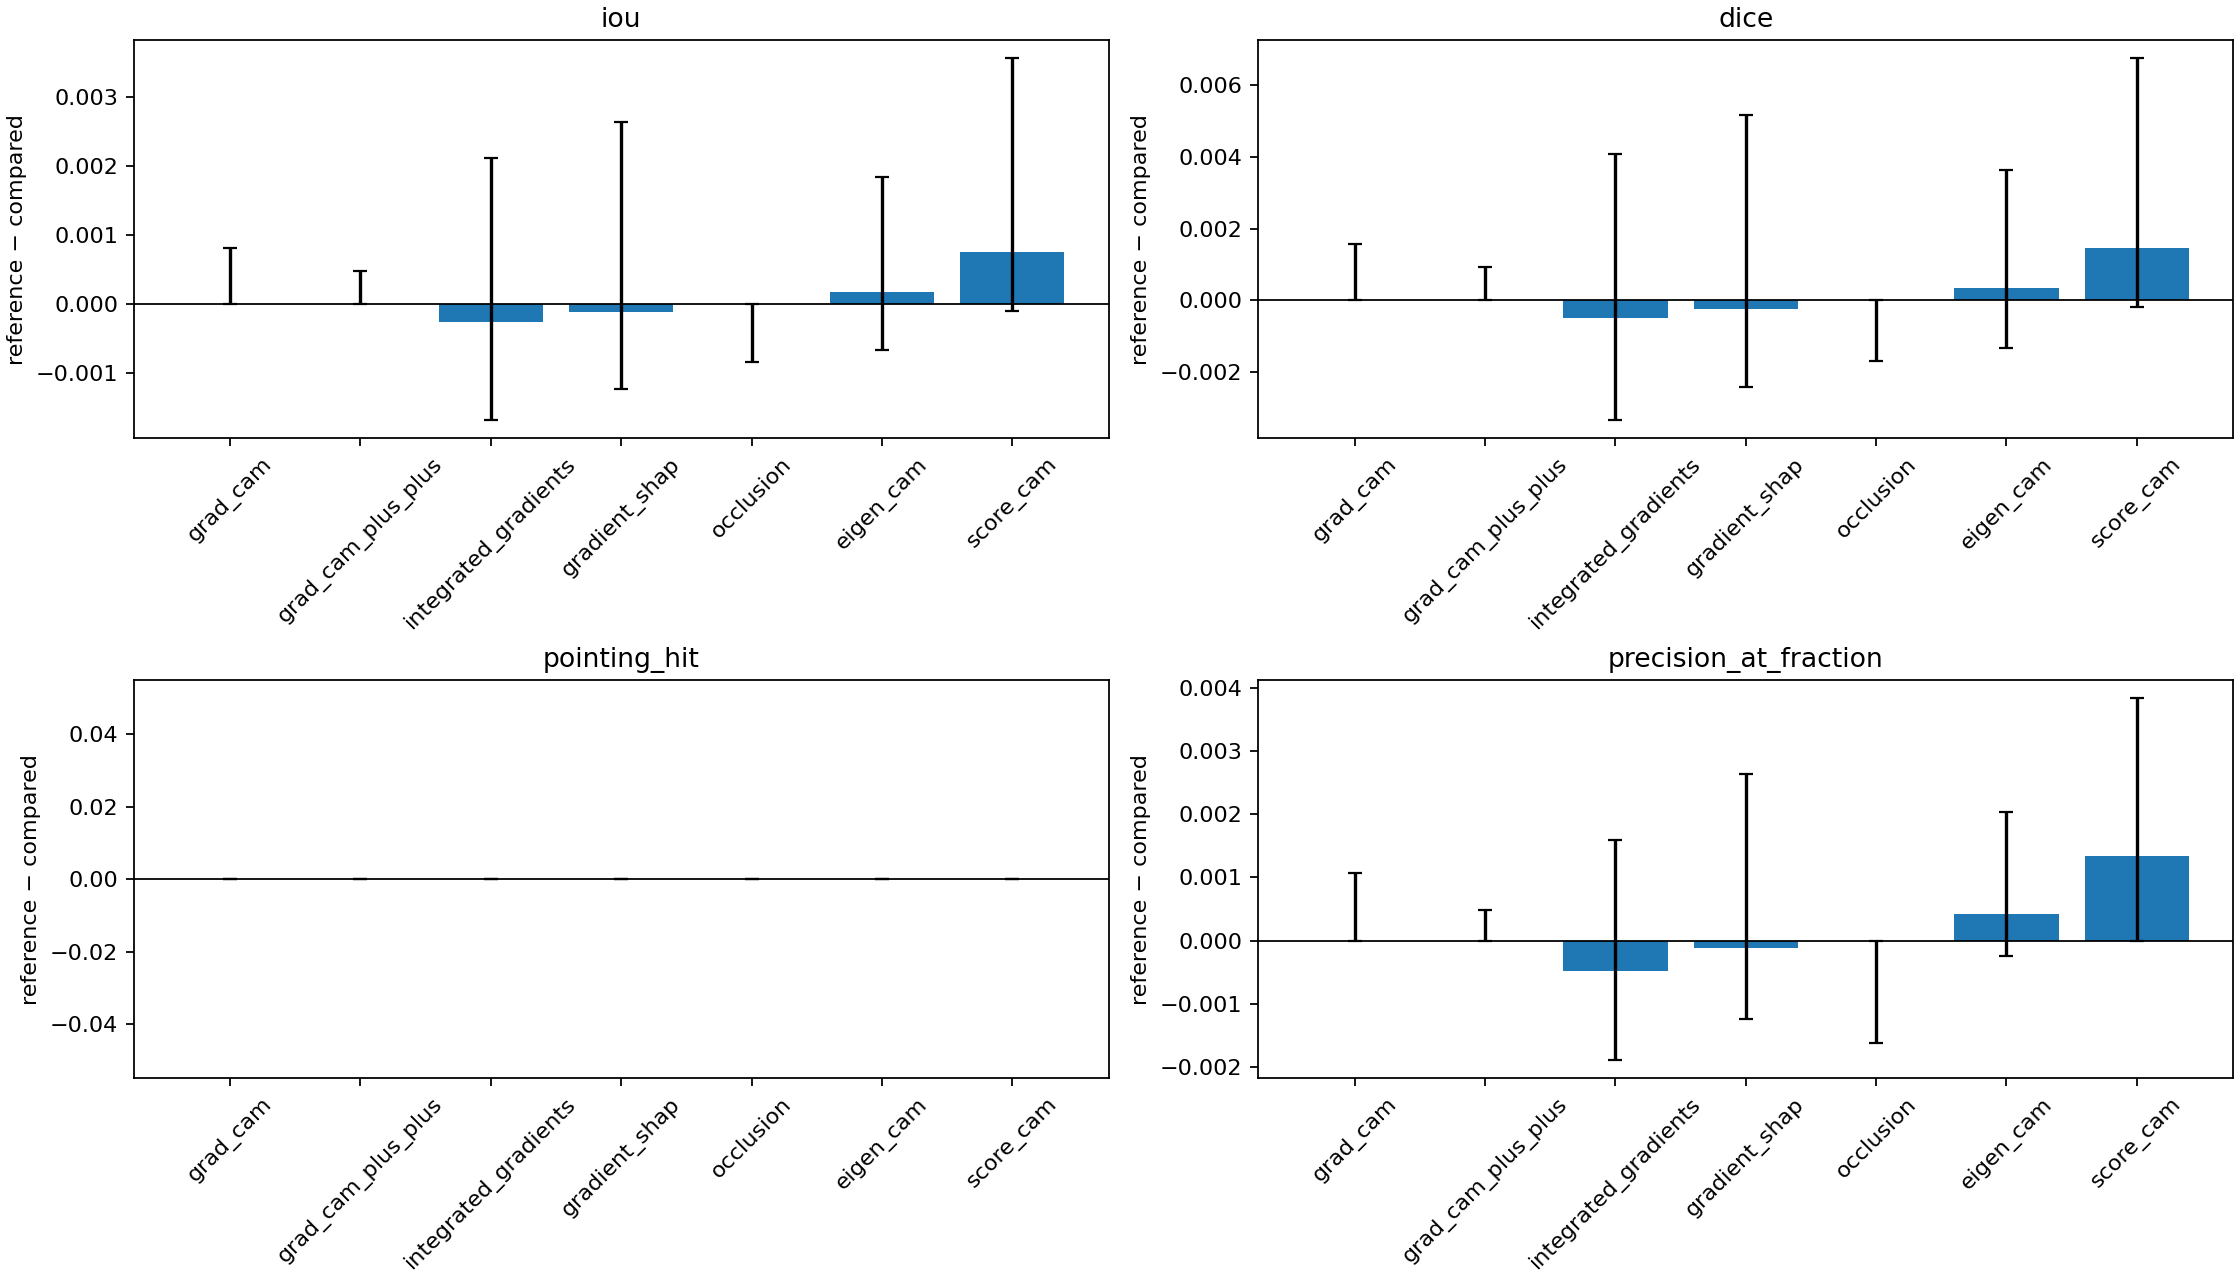
\includegraphics[width=0.945\linewidth,height=0.28\textheight,keepaspectratio]{figures/iter_58_chex_improvement_v3__improvement_experiment_paired_diff.png}%
		\subcaption{CheXpert model}
	\end{minipage}

	\vspace{1em} % controlled spacing between rows

	% --- Row 2 ---
	\begin{minipage}{\linewidth}
		\centering
		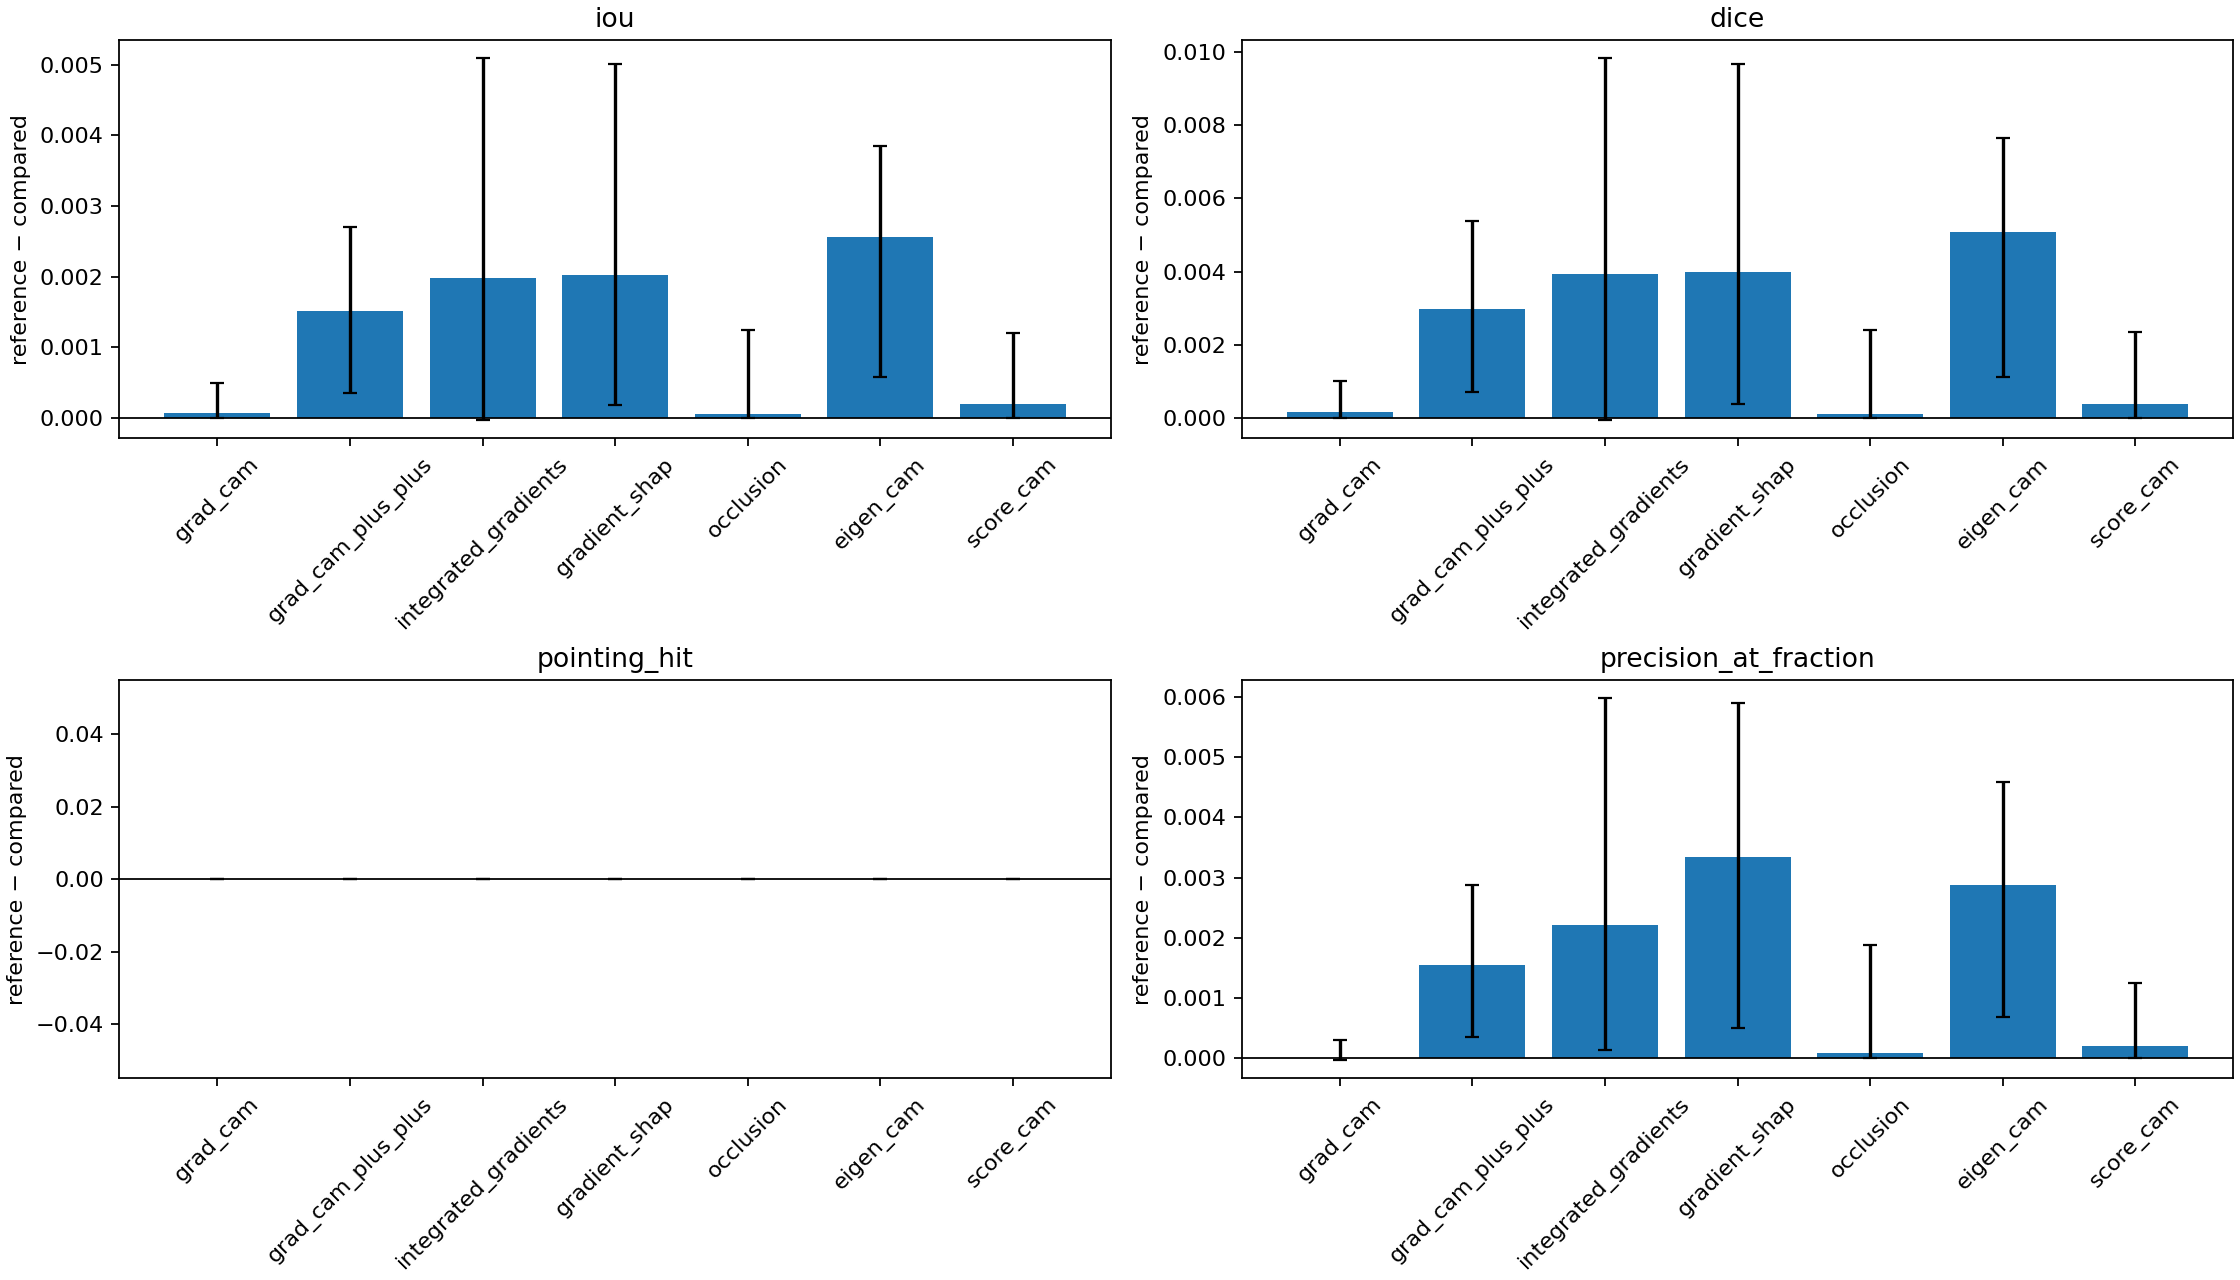
\includegraphics[width=0.945\linewidth,height=0.28\textheight,keepaspectratio]{figures/iter_52_resnet_improvement_v3__improvement_experiment_paired_diff.png}%
		\subcaption{ResNet model}
	\end{minipage}
	
	\vspace{1em}
	
	% --- Row 3 ---
	\begin{minipage}{\linewidth}
		\centering
		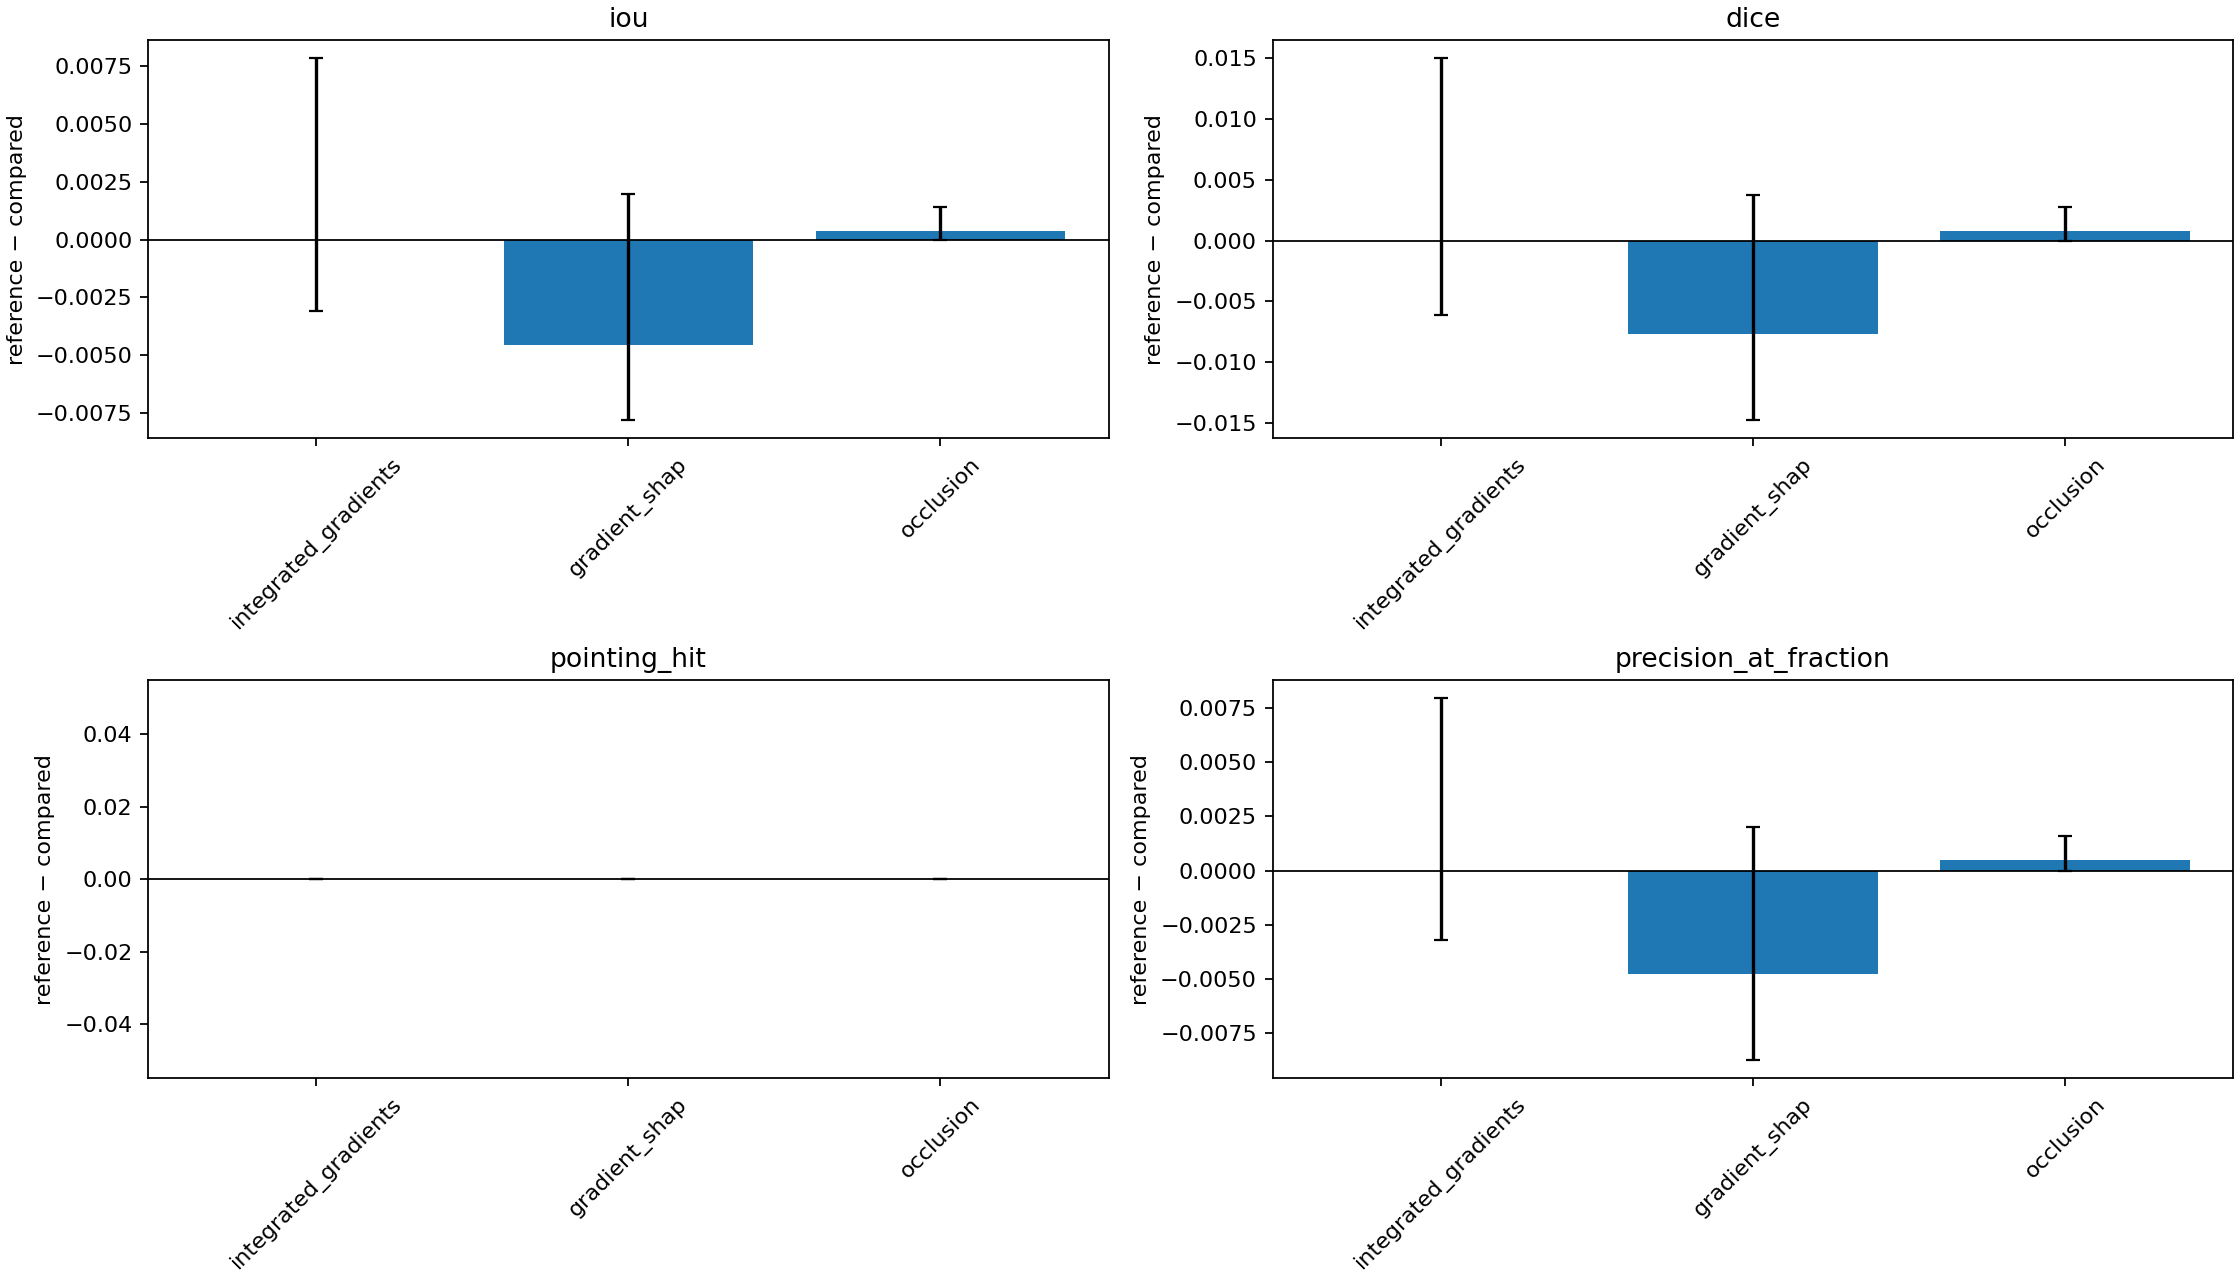
\includegraphics[width=0.945\linewidth,height=0.28\textheight,keepaspectratio]{figures/iter_54_ct_improvement_test__ct_improvement_experiment_paired_diff.png}%
		\subcaption{CT model}
	\end{minipage}
	
	\vspace{1em}
	
	% --- main caption for the whole figure ---
	\caption{Paired consensus-vs-individual localization differences}
	\label{graph:4-5}
\end{graph}

\begingroup
\setlength{\tabcolsep}{4pt}
\renewcommand{\arraystretch}{1.15}
\begin{longtable}[]{@{}
		>{\raggedright\arraybackslash}p{0.20\textwidth}
		>{\raggedright\arraybackslash}p{0.22\textwidth}
		>{\raggedright\arraybackslash}p{0.48\textwidth}
		@{}}
	\caption{Improvement-experiment paired Dice comparison}\label{table:4-6}\tabularnewline
	\toprule
	Model & Method compared with frozen consensus & Dice statistics\tabularnewline
	\midrule
	\endfirsthead
	\toprule
	Model & Method compared with frozen consensus & Dice statistics\tabularnewline
	\midrule
	\endhead
	\texttt{densenet121-\allowbreak res224-\allowbreak chex} & Grad-CAM &
	Consensus median: \texttt{0.0211}\newline
	Method median: \texttt{0.0222}\newline
	Median paired difference: \texttt{0.0000}\newline
	95\% bootstrap CI: \texttt{[0.0000, 0.0016]}\newline
	Wilcoxon p: \texttt{0.0441}\newline
	Holm-adjusted p: \texttt{0.2205}\newline
	Interpretation: not significant\tabularnewline
	\midrule
	\texttt{densenet121-\allowbreak res224-\allowbreak chex} & Grad-CAM++ &
	Consensus median: \texttt{0.0211}\newline
	Method median: \texttt{0.0127}\newline
	Median paired difference: \texttt{0.0000}\newline
	95\% bootstrap CI: \texttt{[0.0000, 0.0009]}\newline
	Wilcoxon p: \texttt{0.8024}\newline
	Holm-adjusted p: \texttt{0.8024}\newline
	Interpretation: not significant\tabularnewline
	\midrule
	\texttt{densenet121-\allowbreak res224-\allowbreak chex} & Integrated Gradients &
	Consensus median: \texttt{0.0211}\newline
	Method median: \texttt{0.0226}\newline
	Median paired difference: \texttt{-0.0005}\newline
	95\% bootstrap CI: \texttt{[-0.0033, 0.0041]}\newline
	Wilcoxon p: \texttt{0.1972}\newline
	Holm-adjusted p: \texttt{0.3945}\newline
	Interpretation: not significant\tabularnewline
	\midrule
	\texttt{densenet121-\allowbreak res224-\allowbreak chex} & GradientSHAP &
	Consensus median: \texttt{0.0211}\newline
	Method median: \texttt{0.0213}\newline
	Median paired difference: \texttt{-0.0002}\newline
	95\% bootstrap CI: \texttt{[-0.0024, 0.0052]}\newline
	Wilcoxon p: \texttt{0.0499}\newline
	Holm-adjusted p: \texttt{0.2205}\newline
	Interpretation: not significant\tabularnewline
	\midrule
	\texttt{densenet121-\allowbreak res224-\allowbreak chex} & Occlusion &
	Consensus median: \texttt{0.0211}\newline
	Method median: \texttt{0.0191}\newline
	Median paired difference: \texttt{0.0000}\newline
	95\% bootstrap CI: \texttt{[-0.0017, 0.0000]}\newline
	Wilcoxon p: \texttt{0.1111}\newline
	Holm-adjusted p: \texttt{0.3333}\newline
	Interpretation: not significant\tabularnewline
	\midrule
	\texttt{densenet121-\allowbreak res224-\allowbreak chex} & Eigen-CAM &
	Consensus median: \texttt{0.0211}\newline
	Method median: \texttt{0.0186}\newline
	Median paired difference: \texttt{0.0004}\newline
	95\% bootstrap CI: \texttt{[-0.0013, 0.0036]}\newline
	Wilcoxon p: \texttt{0.0309}\newline
	Holm-adjusted p: \texttt{0.1855}\newline
	Interpretation: not significant\tabularnewline
	\midrule
	\texttt{densenet121-\allowbreak res224-\allowbreak chex} & Score-CAM &
	Consensus median: \texttt{0.0211}\newline
	Method median: \texttt{0.0190}\newline
	Median paired difference: \texttt{0.0015}\newline
	95\% bootstrap CI: \texttt{[-0.0002, 0.0068]}\newline
	Wilcoxon p: \texttt{0.0005}\newline
	Holm-adjusted p: \texttt{0.0033}\newline
	Interpretation: significant, small effect\tabularnewline
	\midrule
	\texttt{resnet50-\allowbreak res512-\allowbreak all} & Grad-CAM &
	Consensus median: \texttt{0.0218}\newline
	Method median: \texttt{0.0172}\newline
	Median paired difference: \texttt{0.0001}\newline
	95\% bootstrap CI: \texttt{[0.0000, 0.0010]}\newline
	Wilcoxon p: \texttt{0.6000}\newline
	Holm-adjusted p: \texttt{0.9789}\newline
	Interpretation: not significant\tabularnewline
	\midrule
	\texttt{resnet50-\allowbreak res512-\allowbreak all} & Grad-CAM++ &
	Consensus median: \texttt{0.0218}\newline
	Method median: \texttt{0.0085}\newline
	Median paired difference: \texttt{0.0030}\newline
	95\% bootstrap CI: \texttt{[0.0007, 0.0054]}\newline
	Wilcoxon p: \texttt{0.0002}\newline
	Holm-adjusted p: \texttt{0.0006}\newline
	Interpretation: significant\tabularnewline
	\midrule
	\texttt{resnet50-\allowbreak res512-\allowbreak all} & Integrated Gradients &
	Consensus median: \texttt{0.0218}\newline
	Method median: \texttt{0.0184}\newline
	Median paired difference: \texttt{0.0039}\newline
	95\% bootstrap CI: \texttt{[-0.0001, 0.0098]}\newline
	Wilcoxon p: \texttt{\textless0.0001}\newline
	Holm-adjusted p: \texttt{\textless0.0001}\newline
	Interpretation: significant\tabularnewline
	\midrule
	\texttt{resnet50-\allowbreak res512-\allowbreak all} & GradientSHAP &
	Consensus median: \texttt{0.0218}\newline
	Method median: \texttt{0.0183}\newline
	Median paired difference: \texttt{0.0040}\newline
	95\% bootstrap CI: \texttt{[0.0004, 0.0097]}\newline
	Wilcoxon p: \texttt{\textless0.0001}\newline
	Holm-adjusted p: \texttt{\textless0.0001}\newline
	Interpretation: significant\tabularnewline
	\midrule
	\texttt{resnet50-\allowbreak res512-\allowbreak all} & Occlusion &
	Consensus median: \texttt{0.0218}\newline
	Method median: \texttt{0.0252}\newline
	Median paired difference: \texttt{0.0001}\newline
	95\% bootstrap CI: \texttt{[0.0000, 0.0024]}\newline
	Wilcoxon p: \texttt{0.0139}\newline
	Holm-adjusted p: \texttt{0.0416}\newline
	Interpretation: significant, very small effect\tabularnewline
	\midrule
	\texttt{resnet50-\allowbreak res512-\allowbreak all} & Eigen-CAM &
	Consensus median: \texttt{0.0218}\newline
	Method median: \texttt{0.0139}\newline
	Median paired difference: \texttt{0.0051}\newline
	95\% bootstrap CI: \texttt{[0.0011, 0.0076]}\newline
	Wilcoxon p: \texttt{\textless0.0001}\newline
	Holm-adjusted p: \texttt{0.0002}\newline
	Interpretation: significant\tabularnewline
	\midrule
	\texttt{resnet50-\allowbreak res512-\allowbreak all} & Score-CAM &
	Consensus median: \texttt{0.0218}\newline
	Method median: \texttt{0.0144}\newline
	Median paired difference: \texttt{0.0004}\newline
	95\% bootstrap CI: \texttt{[0.0000, 0.0024]}\newline
	Wilcoxon p: \texttt{0.4894}\newline
	Holm-adjusted p: \texttt{0.9789}\newline
	Interpretation: not significant\tabularnewline
	\bottomrule
\end{longtable}
\endgroup

The table \ref{table:4-6} should be read together with the aggregate means. For
DenseNet-chex, consensus is statistically better than
Score-CAM by Dice, IoU and precision, but it is not the best method
by aggregate mean Dice (Occlusion and
Grad-CAM++ are slightly higher descriptively). For
ResNet-50, consensus is statistically better than several methods by
Dice/IoU, but Grad-CAM and Score-CAM remain
competitive and the absolute overlap remains weak. 

This supports a
specific conclusion: consensus can stabilize localization when individual
methods are noisy or weak, but it is not a substitute for a clinically
aligned classifier.

\hypertarget{limitations}{%
	\section{Limitations}\label{limitations}}

Due to time constraints the scope of this study was significantly limited 
and lead to certain limitations to consider as well as model-specific 
restrictions.

\textbf{Internal validity.} The results depend on preprocessing, image
size, classifier threshold, XAI hyperparameters, top-fraction
calibration, smoothing, perturbation baseline, and random sampling. This
study controls these risks by freezing classifier thresholds, using
fixed seeds, versioning calibration artifacts, and reporting method
settings. However, small changes in baseline choice or smoothing can
alter pixel-level attribution maps, especially for
Integrated Gradients and GradientSHAP. Long-running
experiments also use practical speed settings such as capped
Score-CAM channels or coarse occlusion patches; 
more resource-heavy reruns should replace the results were such approximations
were used since the resulting scores and metrics may differ significantly for 
these specific XAI methods.

\textbf{Construct validity.} Pneumothorax masks are useful reference
annotations, but they are imperfect proxies for explanation quality. A
model may highlight clinically related indirect evidence such as
mediastinal shifts, mixed lower mediastinal and intrapleural air, 
collapsed parts of the lungs with appropriately deformed roots,
which will not overlap the mask by design. 
Conversely, a heatmap may overlap the mask for non-causal or
due to high diffusion and non-specificity of the gradient. 
Therefore, mask metrics are interpreted as
localization evidence, not as complete clinical validity. Negative
evidence is also a separate construct: overlap between suppressive
evidence and the lesion itself should be viewed outside of the context 
of its weight and the input from other maps.

\textbf{External validity.} The tested CXR models are off-the-shelf
TorchXRayVision classifiers, not SIIM-specific pneumothorax localization
models. Low mask overlap may reflect model/data mismatch, low quality masks, 
report-label pretraining, or transfer-distribution shift
\cite{ref-cxr-generalization-zech} as much as explanation-method
failure. The model sweep improves this limitation by comparing
several TorchXRayVision weights and architectures, but the out-of-family
external-model slot remains unresolved because the checked MONAI CXR
candidate was generative rather than a pneumothorax classifier. The
results should therefore be viewed as evidence about this off-the-shelf
model family on SIIM pneumothorax, not as a universal claim about all
CXR AI systems.

\textbf{Statistical validity.} The balanced ResNet review is a
single-rater, 40-case, outcome-stratified study with 10 \texttt{tp}, 10
\texttt{fp}, 10 \texttt{tn}, and 10 \texttt{fn} cases. It is exploratory
by design and is not a powered multi-rater reader study. There is no
inter-rater reliability statistic, no formal clinical-deployment
validation, and no prospective workflow assessment. Review-score
correlations and cross-case pattern-similarity observations should
therefore be described as supporting qualitative evidence rather than
definitive statistical proof. 

\textbf{Visualization and interpretation limits.} Heatmap readability
depends on color mapping, selected view, selected top fraction,
smoothing, and overlay opacity. All thesis attribution maps are
class-specific model-evidence visualizations. 
Faithfulness curves have a related limitation: they
evaluate sensitivity of the model output to a perturbation design, so
their clinical meaning depends on whether the replacement baseline is
appropriate for the modality as well as the quality of the model itself.

\textbf{Scope limits.} The CT component is not a full
second clinical validation study. It uses one PhysioNet CT hemorrhage
dataset, one DifeiT ViT checkpoint, positive masked slices, and
input-space explanation methods only. The CXR and CT consensus
definitions also differ: CXR uses the frozen four-method consensus,
whereas CT uses a three-method consensus, because the convolutional CAM
implementations do not directly apply to the Vision Transformer.

\hypertarget{conclusions-to-chapter-4}{%
	\section*{Conclusions to Chapter 4}\label{conclusions-to-chapter-4}}
\addcontentsline{toc}{section}{Conclusions to Chapter 4}

Chapter 4 shows that the evaluation of explanations must be separated
from the evaluation of classifier predictions. The 
DenseNet-chex is the selected DenseNet baseline and
\texttt{resnet50-\allowbreak res512-\allowbreak all} is the strongest tested TorchXRayVision
models by aggregate localization. However, the absolute localization
values remain low.

The quantitative explanation results should be interpreted through
complementary metrics. \texttt{IoU}, \texttt{Dice}, and
\texttt{precision \allowbreak at \allowbreak fraction} describe selected-region overlap with
the target mask, while \texttt{pointing \allowbreak hit} is a stricter
peak-localization diagnostic. Signed diagnostics and negative-evidence
measures answer a different question and should not be collapsed into
positive lesion-overlap scores. Faithfulness curves add another layer
of information by
testing whether highlighted pixels affect the model output under
deletion or insertion, but they do not prove that the highlighted
evidence is clinically appropriate.

The balanced 40-case ResNet review provides the strongest qualitative
CXR evidence currently available. It shows that explanations can be
useful or potentially useful in many cases, but clinically misleading
and poorly localized maps remain common. Non-pathological high-contrast
evidence, device/tube confounding, indirect clinically related signs,
method disagreement, weak pixel attribution, subcutaneous emphysema, and
mask-quality concerns all affect interpretation. The improvement experiments 
add that consensus behavior is model-,
metric-, and modality-dependent: for DenseNet-chex it mainly improves
over Score-CAM in paired overlap tests, for ResNet-50 it improves
Dice/IoU over several weaker methods while remaining comparable to
strong CAM alternatives, and for CT it gives its clearest benefit on
pointing-hit rather than broad overlap. Together, these findings support
the broader point that XAI maps are valuable when they are
validated as model-behavior diagnostics, not when they are displayed as
automatic evidence of trustworthiness.

The CT experiments provide evidence that the existing approaches 
may be transferable, however, they are highly model dependent and 
warrant more future investigation.

\hypertarget{conclusions-and-recommendations}{%
	\chapter{Conclusions and
		Recommendations}\label{conclusions-and-recommendations}}

\hypertarget{main-findings}{%
	\section{Main Findings}\label{main-findings}}

The thesis supports a cautious interpretation of explainable AI in
medical image classification. The main finding is that heatmaps can be
useful for auditing model behavior, but they should not be treated as
automatic evidence of clinical correctness. In the CXR pneumothorax case
study, the tested off-the-shelf TorchXRayVision models can produce
class-specific attribution maps, yet many maps remain weakly localized
to the pneumothorax masks or highlight indirect, confounded, or
high-contrast non-lesion structures.

The model weights comparison shows that model choice matters: 
\texttt{densenet121-\allowbreak res224-\allowbreak chex} improves over the original
\texttt{densenet121-\allowbreak res224-\allowbreak all} checkpoint within the DenseNet-121
branch, while \texttt{resnet50-\allowbreak res512-\allowbreak all} is the strongest tested
TorchXRayVision candidate by aggregate localization in the completed
diagnostic sweep. However, the absolute localization values remain low.
This means the CheX and ResNet-50 results should be interpreted as
better relative baselines, not as clinically strong pneumothorax
localizers for the purposes of this work.

The radiologist-centered review reinforces the quantitative caution. In
the balanced 40-case ResNet review, explanation usefulness was mixed:
many cases contained some interpretable signal, but misleading or poorly
localized maps remained common. Non-pathological high-contrast evidence,
device/tube confounding, indirect evidence, method disagreement, weak
pixel attribution, subcutaneous emphysema, and mask-quality issues all
appeared as clinically relevant interpretation factors. These findings
support the thesis claim that XAI is most valuable when used to expose
model limitations rather than to create trust automatically.

The consensus-improvement experiment shows that consensus is
not universally superior. In the DenseNet-chex baseline, the frozen
consensus significantly improves overlap mainly over
Score-CAM, while Occlusion and
Grad-CAM++ remain slightly higher by aggregate mean
Dice. In the ResNet-50 baseline, consensus significantly improves
Dice/IoU over several weaker methods, but not over Grad-CAM or
Score-CAM. This supports a model-dependent conclusion:
cross-method consensus can stabilize localization under some baselines,
but averaging weak or mislocalized evidence does not automatically
produce clinically aligned explanations. The methodological contribution
remains that explanation claims should be evaluated through classifier
behavior, localization, faithfulness, method agreement, and clinical
review together.

The completed CT experiment extends this conclusion across modality without
turning it into a universal consensus claim. On positive masked CT
hemorrhage slices, the three-method consensus significantly improves
\texttt{pointing \allowbreak hit} over all three input-space constituent methods,
but its overlap metrics are not Holm-significantly better than
individual methods. The result is useful because it shows that the same
validation framework can be executed beyond CXR and can reveal a
different consensus signature; it remains limited by a single CT
model/dataset, a calibration-floor effect at top fraction \texttt{0.\allowbreak 05},
and the absence of transformer-specific CAM methods in this
thesis.

\hypertarget{practical-recommendations}{%
	\section{Practical Recommendations}\label{practical-recommendations}}

The first practical recommendation is to report classifier performance
and explanation quality separately. A model's \texttt{AUC}, sensitivity,
specificity, or F1 score should not be used as a substitute for evidence
that the model localizes pathology. Conversely, a poor localization
score should be interpreted in relation to the model, dataset, target
class, and reference annotation rather than blamed automatically on one
XAI method.

The second recommendation is to keep explanation views semantically
separate. Positive evidence, negative evidence, magnitude, and signed
views answer different questions. Positive evidence can be evaluated
against positive lesion masks; negative evidence should be interpreted
as suppressive evidence. Magnitude maps answer where the image was
influential, not whether the influence supported the disease class.
Signed maps summarize the balance between positive and negative evidence
but should not replace the separate views.

The third recommendation is to use multiple validation layers. For
thesis-scale XAI evaluation, the minimum useful panel is: mask-overlap
metrics (\texttt{IoU}, \texttt{Dice}, \texttt{precision \allowbreak at \allowbreak fraction}),
strict peak localization (\texttt{pointing \allowbreak hit}), faithfulness curves,
signed-evidence diagnostics, method agreement or disagreement, and
structured radiologist review. These layers should be interpreted
together because each has a different failure mode.

The fourth recommendation is to handle pixel-level attribution methods
carefully. Integrated Gradients and GradientSHAP
should be reported with baseline choice, step/sample count, random seed,
smoothing/readability settings, and any cross-case pattern checks. If
such methods produce visually similar maps across unrelated cases, they
should be treated as diagnostic rather than as strong case-specific clinical evidence.

The fifth recommendation is to design review materials for auditability.
Each selected case should preserve the source image, mask or mask
contour, classifier outcome, probability, continuous heatmap views,
thresholded selections, and method settings. This allows a reviewer to
distinguish direct lesion localization, indirect clinically related
evidence, treatment/device confounding, non-pathological high-contrast
structures, and map artifacts.

The sixth recommendation is a extreme need of a validated, standardized,
multi-radiologist reviewed, multi-machine, multi-center masked public datasets 
based on specific region, pathology, modality and other factors,
to be used as a benchmark for future developments in medical vision related
AI tools and the benchmarking workflows for them.

The final practical recommendation is to avoid over-claiming XAI.
Heatmaps are best used as part of a validation and model-audit workflow.
They can identify when a classifier is behaving plausibly, but their
more important thesis role is to show when a model's apparent success is
not supported by clinically expected evidence.

\hypertarget{future-work}{%
	\section{Future Work}\label{future-work}}

Several extensions follow directly from the limitations of the current
work.

First, future work should evaluate stronger pneumothorax-specific or
externally trained classifiers. The current off-the-shelf
TorchXRayVision baselines are useful for auditing transfer behavior, but
a full clinical claim would require models whose development target,
labels, preprocessing, and validation data are closer to SIIM
pneumothorax localization. Any stronger model should undergo the same
protocol: classifier-threshold calibration, XAI top-fraction
calibration, localization metrics, negative-evidence
diagnostics, faithfulness curves, and radiologist-centered review. A
preliminary drop-in probe of an off-the-shelf Vision Transformer
\cite{ref-vit} ChestX-ray14 \cite{ref-chestxray8} classifier confirmed
the same weak-detection and weak, off-lesion localization pattern
observed for the convolutional baselines, so a controlled transformer
comparison (a probe-trained transformer encoder paired with a
token-to-grid CAM adapter so the full method panel transfers) is still 
to be explored.

Second, the CT experiments should be expanded beyond the current 
scope. This thesis verifies one hemorrhage classifier and one mask
source, but a full CT study would add broader test screening, larger or
multi-source annotated hemorrhage masks, subtype-aware analysis,
multi-rater review, and a calibration sweep that extends below top
fraction \texttt{0.\allowbreak 05} for small hemorrhage masks. Candidate future
sources include RSNA-IHD-derived classifier work \cite{ref-rsna-ihd} and
additional public CT hemorrhage datasets with masks, but every extension
must verify class heads, licenses, preprocessing, and data compatibility.

Third, the radiologist review should be scaled beyond the current
single-rater balanced review. A stronger reader study would include
multiple radiologists, inter-rater reliability statistics, a larger and
prospectively defined case sample, blinded scoring, and clearer
separation between direct lesion localization and indirect clinically
relevant evidence. DECIDE-AI-style reporting \cite{ref-decide-ai} would
be appropriate for any study that moves closer to workflow evaluation.

Fourth, additional explanation methods and robustness metrics can be
added. \texttt{LIME} \cite{ref-lime} would provide a region-level
surrogate-family comparator. Captum infidelity and sensitivity metrics
\cite{ref-captum-docs, ref-infidelity-sensitivity} could triangulate
faithfulness and robustness beyond deletion/insertion curves. 

Fifth, an attention-weighted consensus can be explored. This
variant would assign a coefficient $\alpha_m$ to each constituent
method $m$, using possible policies such as calibration-set
mask-IoU, agreement with the method panel, or perturbation stability.
The coefficients would be attention weights across explanation methods,
not architectural attention inside the classifier.

Sixth, the CT experiments can be extended to the CAM-family explanation
methods by adopting transformer-specific spatial-explanation techniques.
Because the integrated CT classifier is a Vision Transformer,
CAM-family methods cannot be applied with the convolutional-feature-map
implementation reused across the chest-X-ray models. Concrete adaptation
paths exist, and their exclusion from this thesis is a deliberate
methodological choice rather than an oversight: the widely-used
\texttt{pytorch-\allowbreak grad-\allowbreak cam} library \cite{ref-pytorch-gradcam} exposes a
token-to-grid reshape that runs CAM-family methods on Vision
Transformers; \texttt{ViT-\allowbreak CX} \cite{ref-vit-cx} provides a
transformer-specific, Score-CAM-style causal explanation built on patch
embeddings; and transformer-native methods such as attention rollout
\cite{ref-attention-rollout} and transformer attribution
\cite{ref-transformer-attribution} explain Vision Transformers through
attention flow and relevance propagation. Each of these is, however, a
different implementation from the convolutional chest-X-ray code path,
so adopting one would re-introduce an implementation variable into a
comparison whose strength is that the explanation algorithm is held
constant across modalities. 
Implementing and validating one of these transformer-specific
approaches in a controlled way would let the full method panel,
including a four-method consensus comparable to the chest-X-ray
definition, be evaluated across both modalities.

Finally, future work should broaden the clinical scope. Additional
pathologies, larger multi-institutional datasets, stronger segmentation
references, and prospective evaluation would test whether the current
cautionary findings generalize. 

\appendix

\hypertarget{experiment-configuration}{%
	\chapter{Experiment Configuration}\label{experiment-configuration}}

This appendix records the configuration required to reproduce the
experiments, so that the main text can remain focused on methodology and
results. It documents the software environment, the dataset composition,
the classifier operating points, and the explanation-method
hyperparameters. The code used to produce these experiments is available
in the repository cited in
Section~\ref{implementation-and-reproducibility}.

The improvement experiment was launched with the command template shown
below; the model weights, input size, and number of positive cases were
substituted per model.

\begingroup
\renewcommand{\FunctionTok}[1]{#1}% template: code in appendices must be all black
\begin{Shaded}
	\begin{Highlighting}[fontsize=\footnotesize,fontfamily=courier]
		\NormalTok{wsl.}\FunctionTok{exe}\NormalTok{ {-}{-}cd /path/to/project python3 scripts/run\_improvementexperiment.}\FunctionTok{py}\NormalTok{ \textasciigrave{}}
		\NormalTok{  {-}{-}weights \textless{}model\_weights\textgreater{} \textasciigrave{}}
		\NormalTok{  {-}{-}image{-}size \textless{}224\_or\_512\textgreater{} \textasciigrave{}}
		\NormalTok{  {-}{-}split test \textasciigrave{}}
		\NormalTok{  {-}{-}max{-}positive \textless{}n\textgreater{} \textasciigrave{}}
		\NormalTok{  {-}{-}random{-}sample \textasciigrave{}}
		\NormalTok{  {-}{-}seed 20260515 \textasciigrave{}}
		\NormalTok{  {-}{-}ig{-}steps 16 \textasciigrave{}}
		\NormalTok{  {-}{-}gradshap{-}samples 8 \textasciigrave{}}
		\NormalTok{  {-}{-}occlusion{-}patch{-}size 32 \textasciigrave{}}
		\NormalTok{  {-}{-}occlusion{-}stride 16 \textasciigrave{}}
		\NormalTok{  {-}{-}score{-}cam{-}channels{-}cap 256 \textasciigrave{}}
		\NormalTok{  {-}{-}calibration{-}csv \textless{}calibrated\_thresholds\_csv\textgreater{} \textasciigrave{}}
		\NormalTok{  {-}{-}device auto \textasciigrave{}}
		\NormalTok{  {-}{-}output{-}dir \textless{}output\_directory\textgreater{}}
	\end{Highlighting}
\end{Shaded}
\endgroup

The software environment, dataset composition, classifier operating
points, and explanation-method hyperparameters are summarised in
Table~\ref{table:a-1}.

\begin{longtable}[]{@{}ll@{}}
	\caption{Experiment configuration summary}\label{table:a-1}\tabularnewline
	\toprule
	\begin{minipage}[b]{0.47\columnwidth}\raggedright
		Configuration item\strut
	\end{minipage} & \begin{minipage}[b]{0.47\columnwidth}\raggedright
		Value\strut
	\end{minipage}\tabularnewline
	\midrule
	\endfirsthead
	\toprule
	\begin{minipage}[b]{0.47\columnwidth}\raggedright
		Configuration item\strut
	\end{minipage} & \begin{minipage}[b]{0.47\columnwidth}\raggedright
		Value\strut
	\end{minipage}\tabularnewline
	\midrule
	\endhead
	Operating environment & Ubuntu under WSL2\tabularnewline
	Python & \texttt{3.10.12}\tabularnewline
	PyTorch & CUDA-enabled build\tabularnewline
	TorchXRayVision & \texttt{1.4.0}\tabularnewline
	\midrule
	SIIM-ACR images & \texttt{12{,}047}\tabularnewline
	SIIM-ACR segmentation masks & \texttt{12{,}047}\tabularnewline
	Positive (pneumothorax) cases & \texttt{2{,}669}\tabularnewline
	Negative cases & \texttt{9{,}378}\tabularnewline
	\midrule
	\texttt{densenet121-\allowbreak res224-\allowbreak chex} operating point & \texttt{0.565}\tabularnewline
	\texttt{resnet50-\allowbreak res512-\allowbreak all} operating point & \texttt{0.525}\tabularnewline
	\texttt{densenet121-\allowbreak res224-\allowbreak all} operating point & \texttt{0.620}\tabularnewline
	\midrule
	Random seed & \texttt{20260515}\tabularnewline
	Integrated Gradients steps & \texttt{16}\tabularnewline
	GradientSHAP samples & \texttt{8}\tabularnewline
	Occlusion patch / stride & \texttt{32} / \texttt{16} px\tabularnewline
	Score-CAM channel cap & \texttt{256}\tabularnewline
	Faithfulness baseline & black image\tabularnewline
	\bottomrule
\end{longtable}

\hypertarget{radiologist-review-template}{%
	\chapter{Radiologist Review
		Template}\label{radiologist-review-template}}

This appendix records the scoring schema used for the structured review,
so that the rater task can be reproduced and audited without access to
the interactive review interface.

The review used a balanced design with the four classifier outcomes
(\texttt{tp}, \texttt{fp}, \texttt{tn}, \texttt{fn}) represented by ten
cases each, for forty cases in total. For every case the reviewer saw
the source image, the reference pneumothorax mask or its contour where
available, the classifier outcome and predicted probability, and the
explanation overlay grid. Each explanation was shown in four views:
positive evidence, negative evidence, magnitude, and the signed view.
The review is a structured qualitative assessment and is not a
prospective clinical validation study.

Each case was scored against the categorical and free-text fields listed
in Table~\ref{table:b-1}. The resulting score distributions are reported
in Table~\ref{table:4-4} and Table~\ref{table:4-5}.

\begin{longtable}[]{@{}
		>{\raggedright\arraybackslash}p{0.22\textwidth}
		>{\raggedright\arraybackslash}p{0.34\textwidth}
		>{\raggedright\arraybackslash}p{0.34\textwidth}@{}}
	\caption{Structured review scoring schema}\label{table:b-1}\tabularnewline
	\toprule
	Field & Permitted values & Description\tabularnewline
	\midrule
	\endfirsthead
	\toprule
	Field & Permitted values & Description\tabularnewline
	\midrule
	\endhead
	\texttt{localization \allowbreak score} &
	correct, partial, incorrect, none &
	Agreement between the highlighted region and the reference
	pneumothorax mask.\tabularnewline
	\midrule
	\texttt{usefulness \allowbreak score} &
	useful, potentially useful, misleading, not useful &
	Clinical usefulness of the explanation to a reader.\tabularnewline
	\midrule
	\texttt{failure \allowbreak category} &
	correct, partial, anatomically related, devices/text artifacts,
	non-pathological high contrast, diffuse non-specific, clinically
	misleading &
	Dominant reason an explanation fails to localize the lesion.\tabularnewline
	\midrule
	\texttt{artifact \allowbreak note} &
	free text &
	Notable imaging artifacts such as tubes, lines, text, or
	markers.\tabularnewline
	\midrule
	\texttt{comment} &
	free text &
	Additional reviewer remarks.\tabularnewline
	\bottomrule
\end{longtable}

\hypertarget{additional-figures}{%
	\chapter{Additional Figures}\label{additional-figures}}

This appendix collects supporting visual examples that complement
Chapter 4. The overlays use the colour conventions introduced earlier:
red marks positive evidence toward the model output, blue marks negative
evidence, violet marks magnitude, and the orange-teal pair marks the
signed map.

Figure~\ref{figure:c-1} shows the consensus-selected evidence region for
one representative case from each classifier outcome, rendered on the
grayscale chest radiograph so that the underlying anatomy stays visible.
Red marks the selected positive evidence and blue the selected negative
evidence at the top-20\% fraction; the green contour outlines the
ground-truth mask where one is present.

\begin{figure}[htbp]
	\centering
	\begin{minipage}{0.48\linewidth}
		\centering
		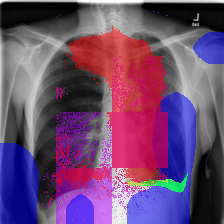
\includegraphics[width=\linewidth,height=0.26\textheight,keepaspectratio]{figures/iter_27__tp__585_test_1__consensus_selected_top_20.png}
		\subcaption{True positive}
	\end{minipage}\hfill
	\begin{minipage}{0.48\linewidth}
		\centering
		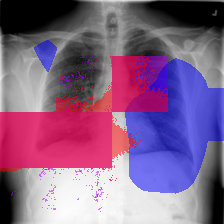
\includegraphics[width=\linewidth,height=0.26\textheight,keepaspectratio]{figures/iter_27__fp__9009_train_0__consensus_selected_top_20.png}
		\subcaption{False positive}
	\end{minipage}

	\vspace{1em}

	\begin{minipage}{0.48\linewidth}
		\centering
		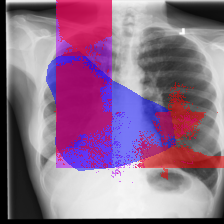
\includegraphics[width=\linewidth,height=0.26\textheight,keepaspectratio]{figures/iter_27__tn__8080_train_0__consensus_selected_top_20.png}
		\subcaption{True negative}
	\end{minipage}\hfill
	\begin{minipage}{0.48\linewidth}
		\centering
		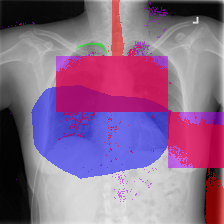
\includegraphics[width=\linewidth,height=0.26\textheight,keepaspectratio]{figures/iter_27__fn__152_test_1__consensus_selected_top_20.png}
		\subcaption{False negative}
	\end{minipage}
	\caption{Representative consensus-selected evidence regions for each classifier outcome}
	\label{figure:c-1}
\end{figure}

Figure~\ref{figure:c-2} illustrates how the selected region changes as
the top-fraction threshold is swept for the consensus map.

\begin{figure}[htbp]
	\centering
	\begin{minipage}{0.9\linewidth}
		\centering
		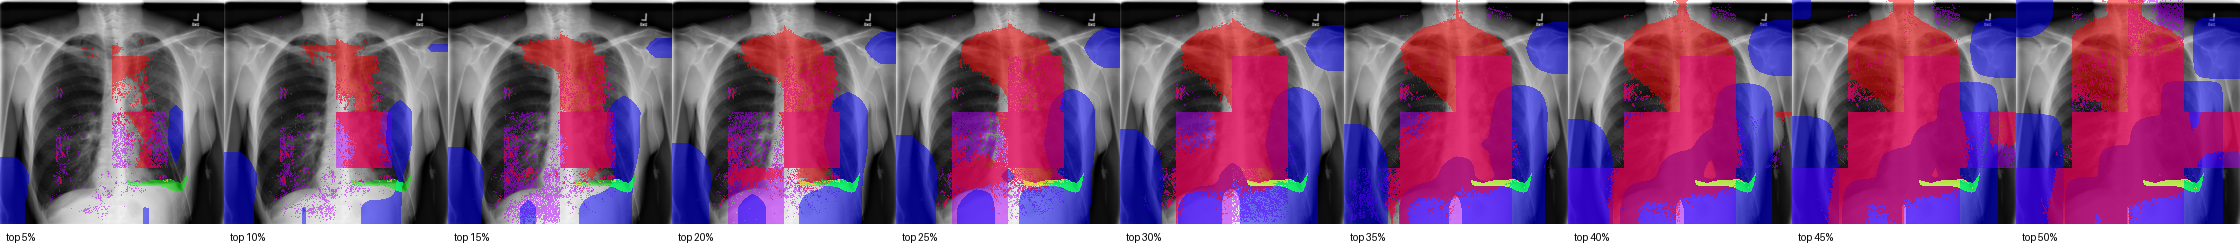
\includegraphics[width=\linewidth,height=0.30\textheight,keepaspectratio]{figures/iter_27__tp__585_test_1__consensus_threshold_sweep_panel.png}
		\subcaption{True-positive case}
	\end{minipage}

	\vspace{1em}

	\begin{minipage}{0.9\linewidth}
		\centering
		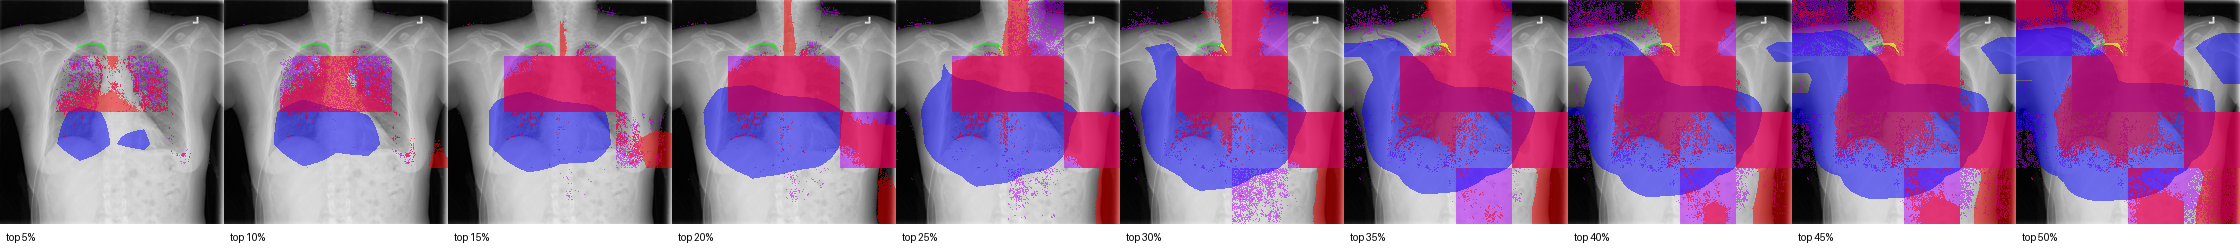
\includegraphics[width=\linewidth,height=0.30\textheight,keepaspectratio]{figures/iter_27__fn__152_test_1__consensus_threshold_sweep_panel.png}
		\subcaption{False-negative case}
	\end{minipage}
	\caption{Consensus top-fraction threshold sweeps}
	\label{figure:c-2}
\end{figure}

Figure~\ref{figure:c-3} reports the paired consensus-versus-individual
Dice distributions for the two CXR baselines.

\begin{figure}[htbp]
	\centering
	\begin{minipage}{\linewidth}
		\centering
		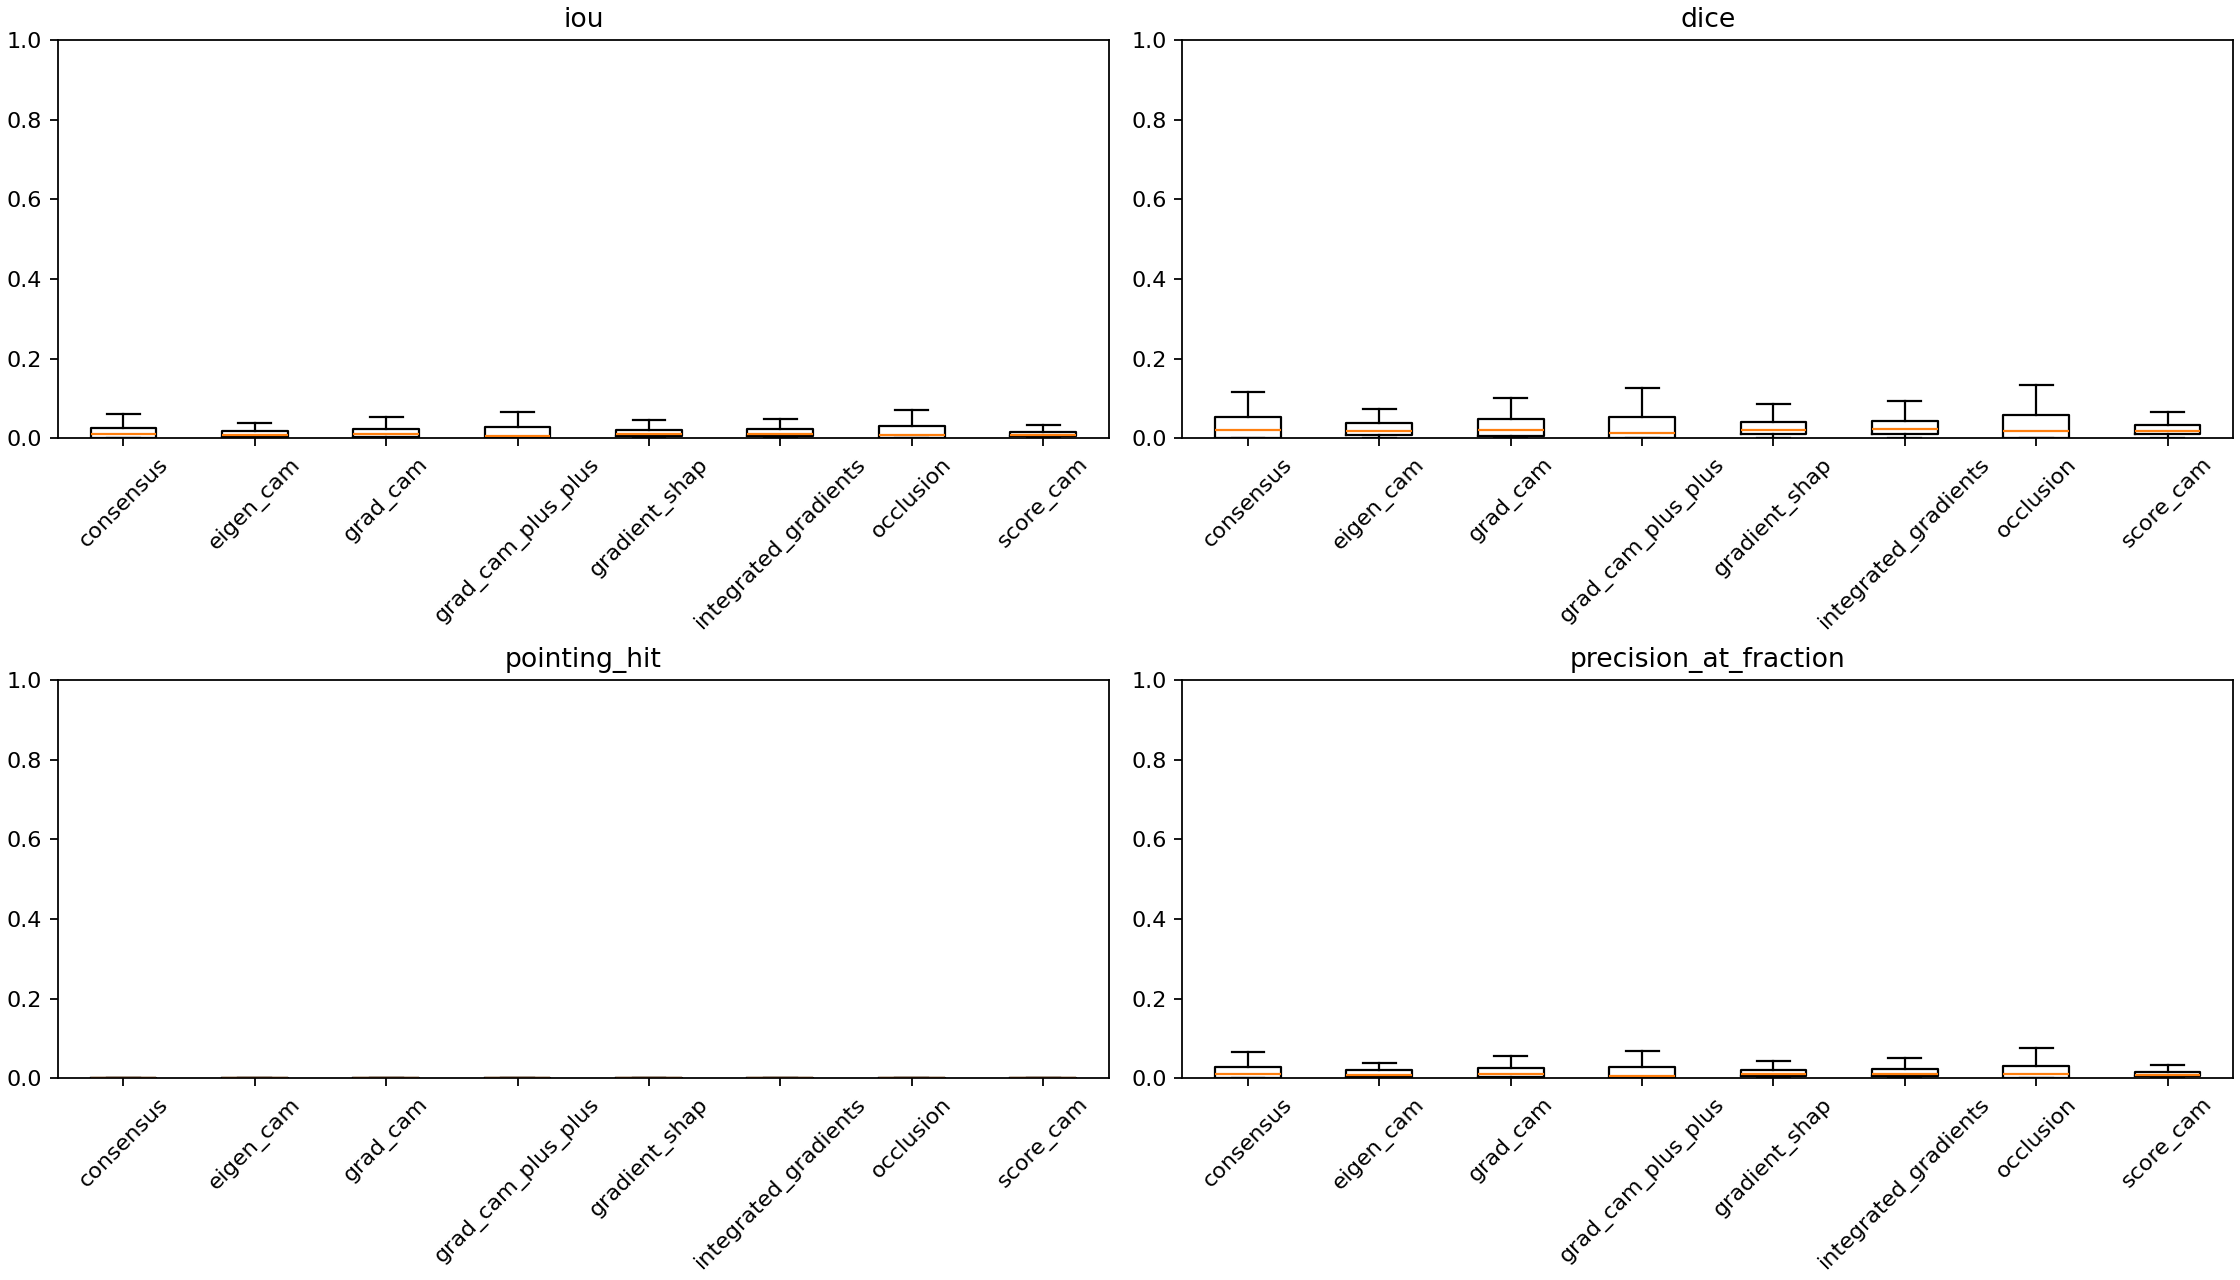
\includegraphics[width=0.85\linewidth,height=0.30\textheight,keepaspectratio]{figures/iter_58_chex_improvement_v3__improvement_experiment_boxplots.png}
		\subcaption{DenseNet-chex}
	\end{minipage}

	\vspace{1em}

	\begin{minipage}{\linewidth}
		\centering
		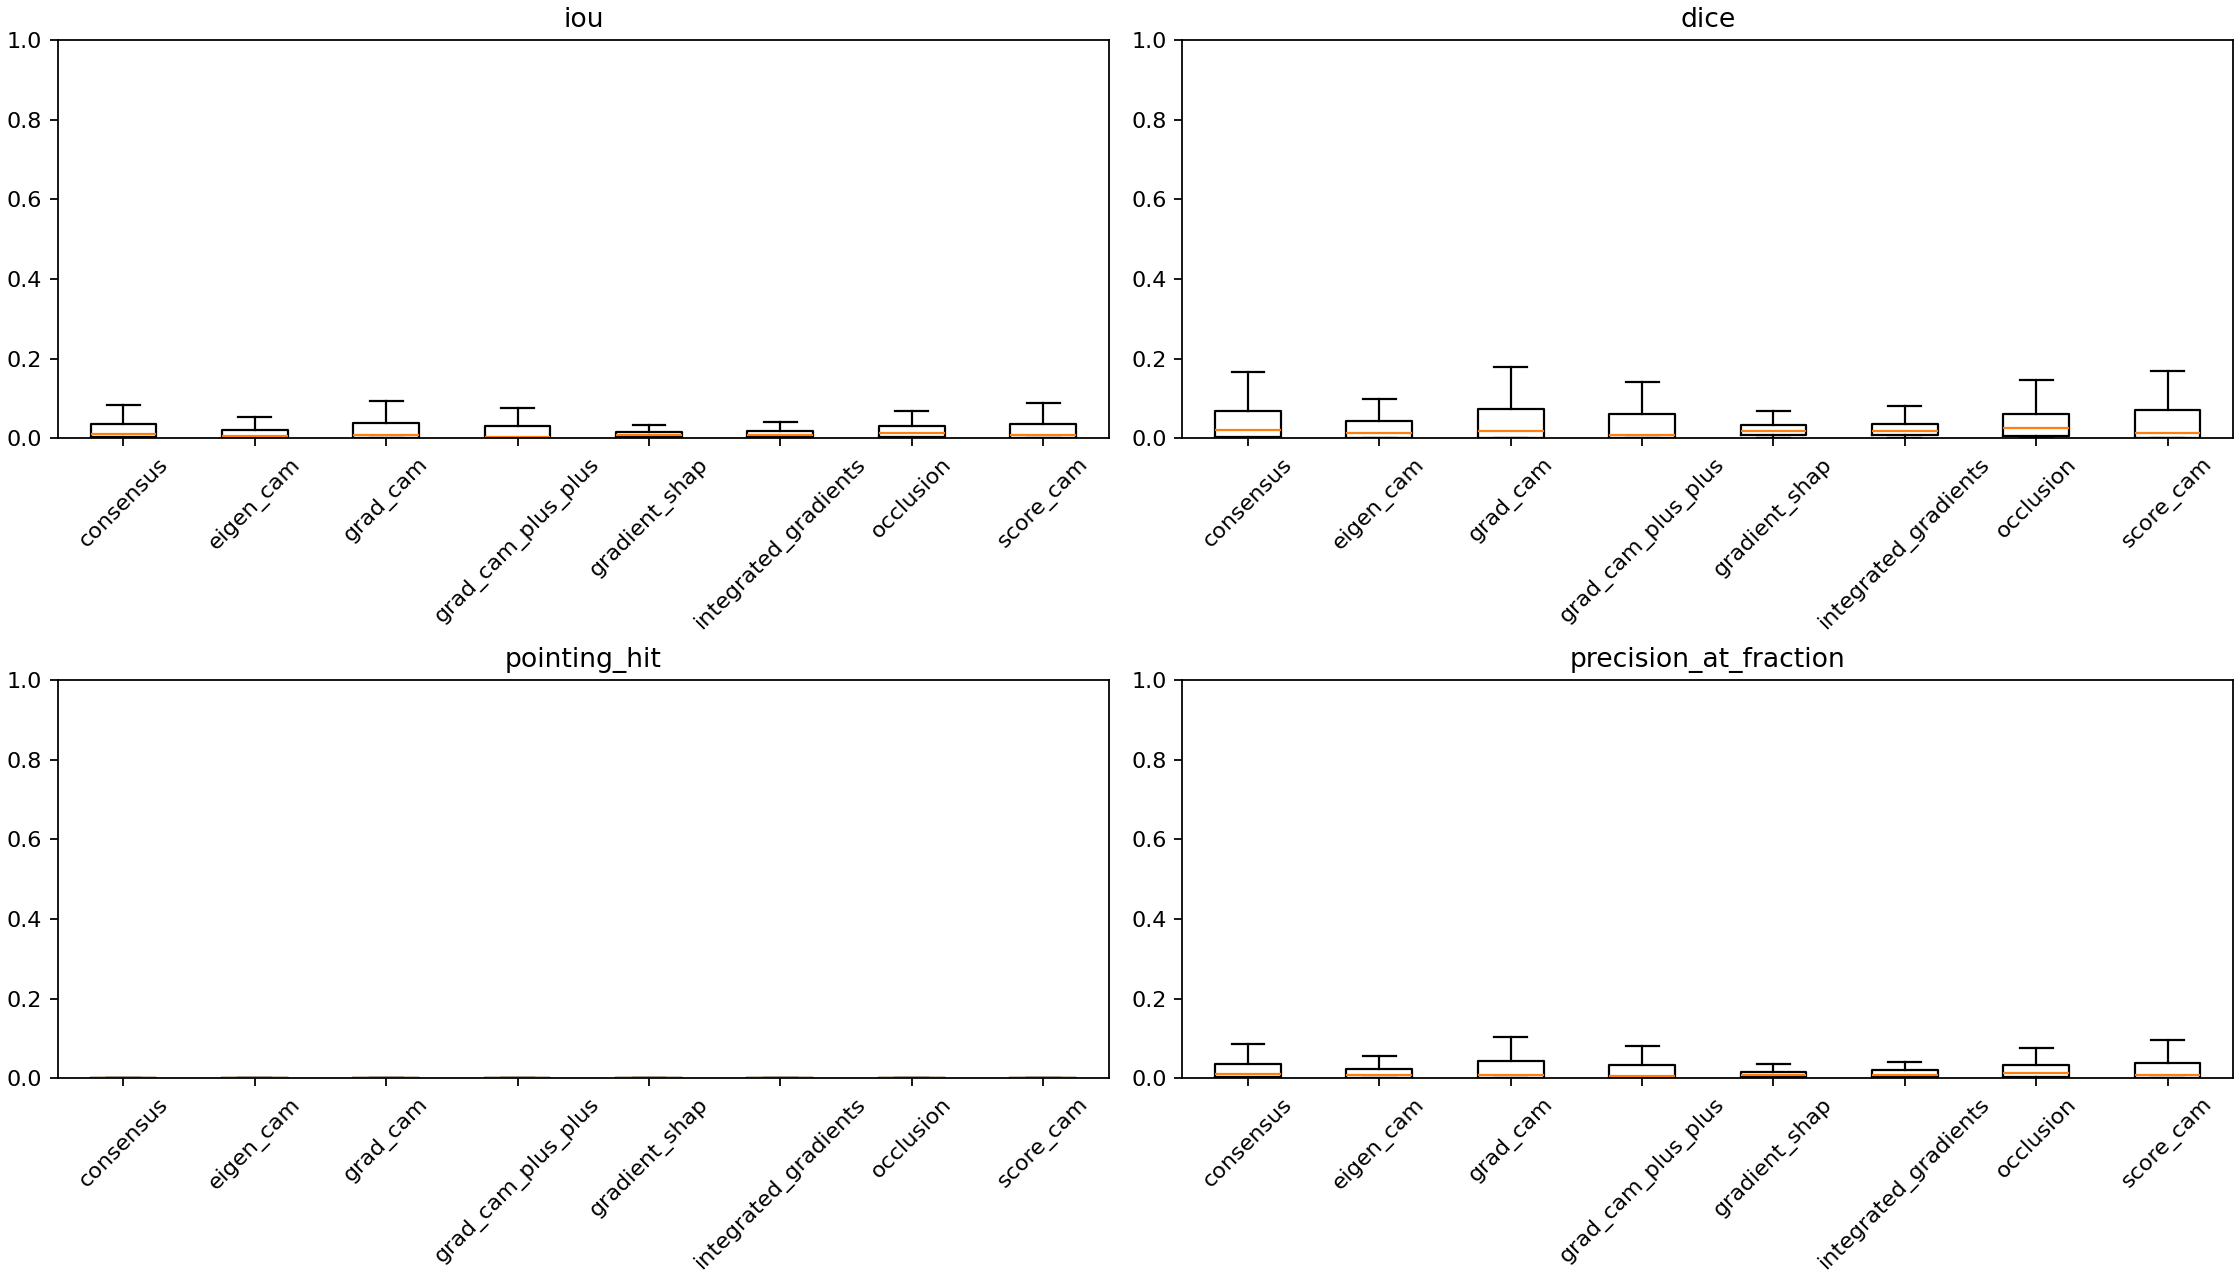
\includegraphics[width=0.85\linewidth,height=0.30\textheight,keepaspectratio]{figures/iter_52_resnet_improvement_v3__improvement_experiment_boxplots.png}
		\subcaption{ResNet-50}
	\end{minipage}
	\caption{Consensus-versus-individual Dice distributions by model}
	\label{figure:c-3}
\end{figure}

Figure~\ref{figure:c-4} shows the deletion and insertion faithfulness
curves for the CT hemorrhage model, including the occlusion-family
detail.

\begin{figure}[htbp]
	\centering
	\begin{minipage}{\linewidth}
		\centering
		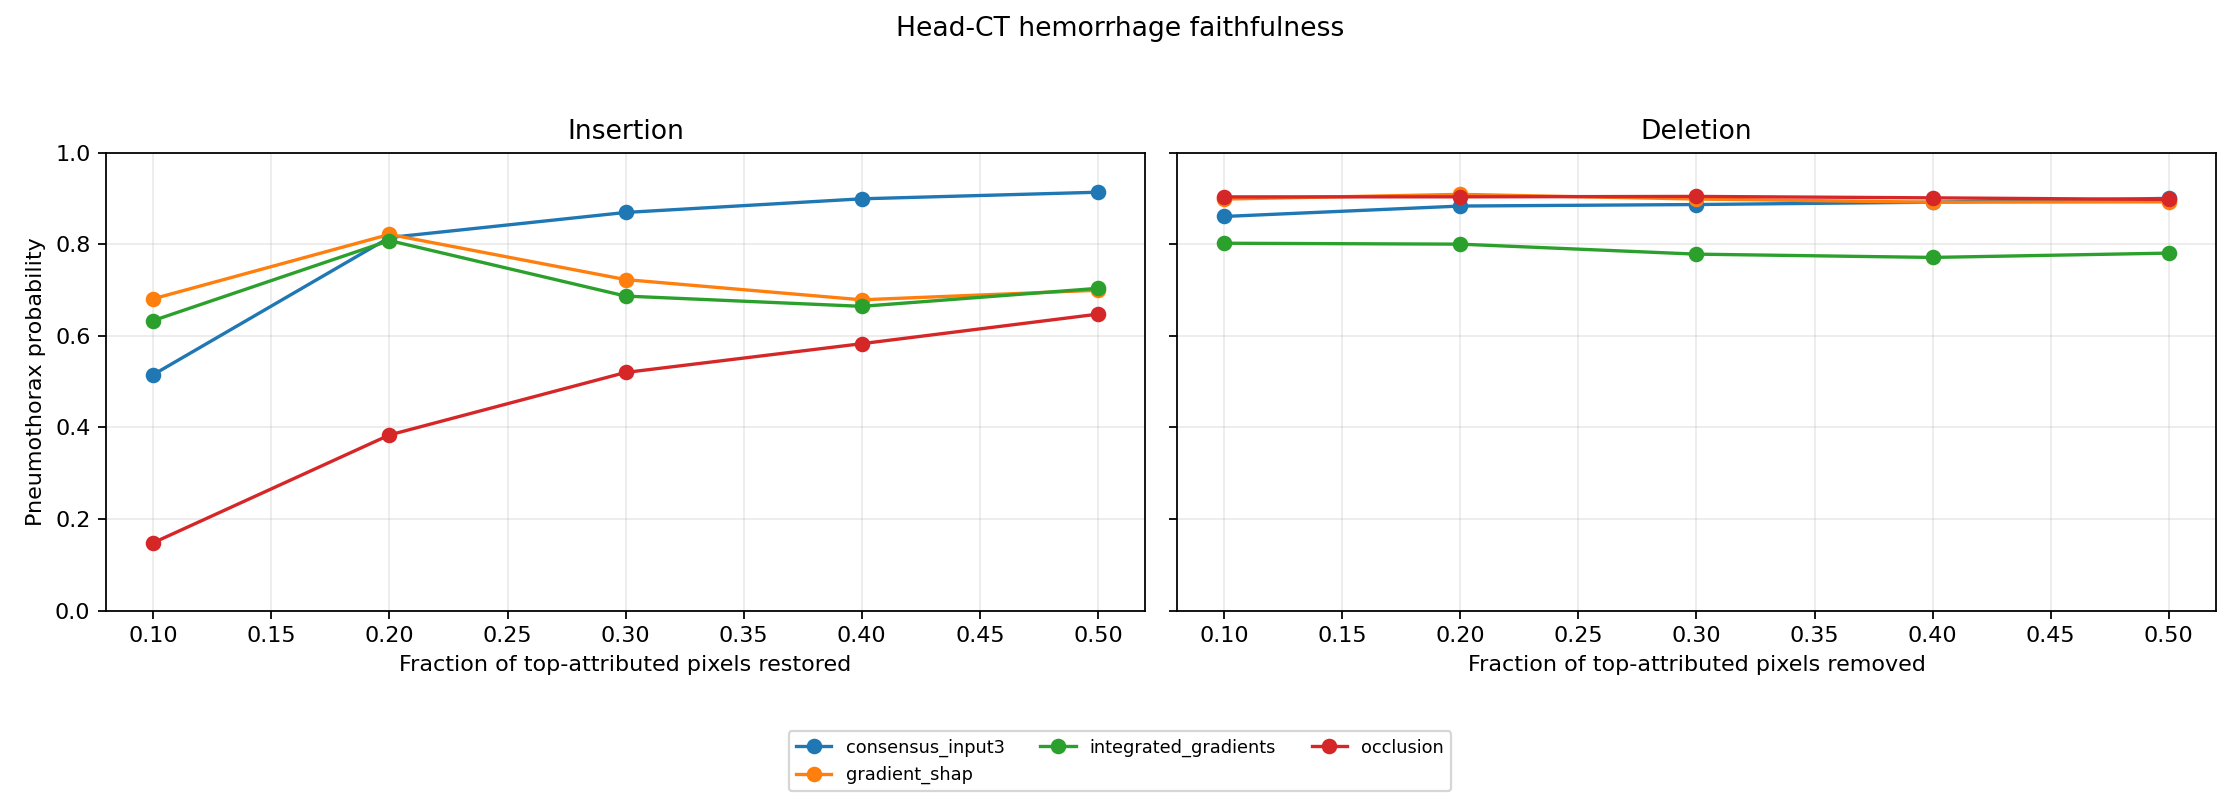
\includegraphics[width=0.85\linewidth,height=0.30\textheight,keepaspectratio]{figures/iter_53_ct_smoke_test__faithfulness_curves.png}
		\subcaption{All methods}
	\end{minipage}

	\vspace{1em}

	\begin{minipage}{\linewidth}
		\centering
		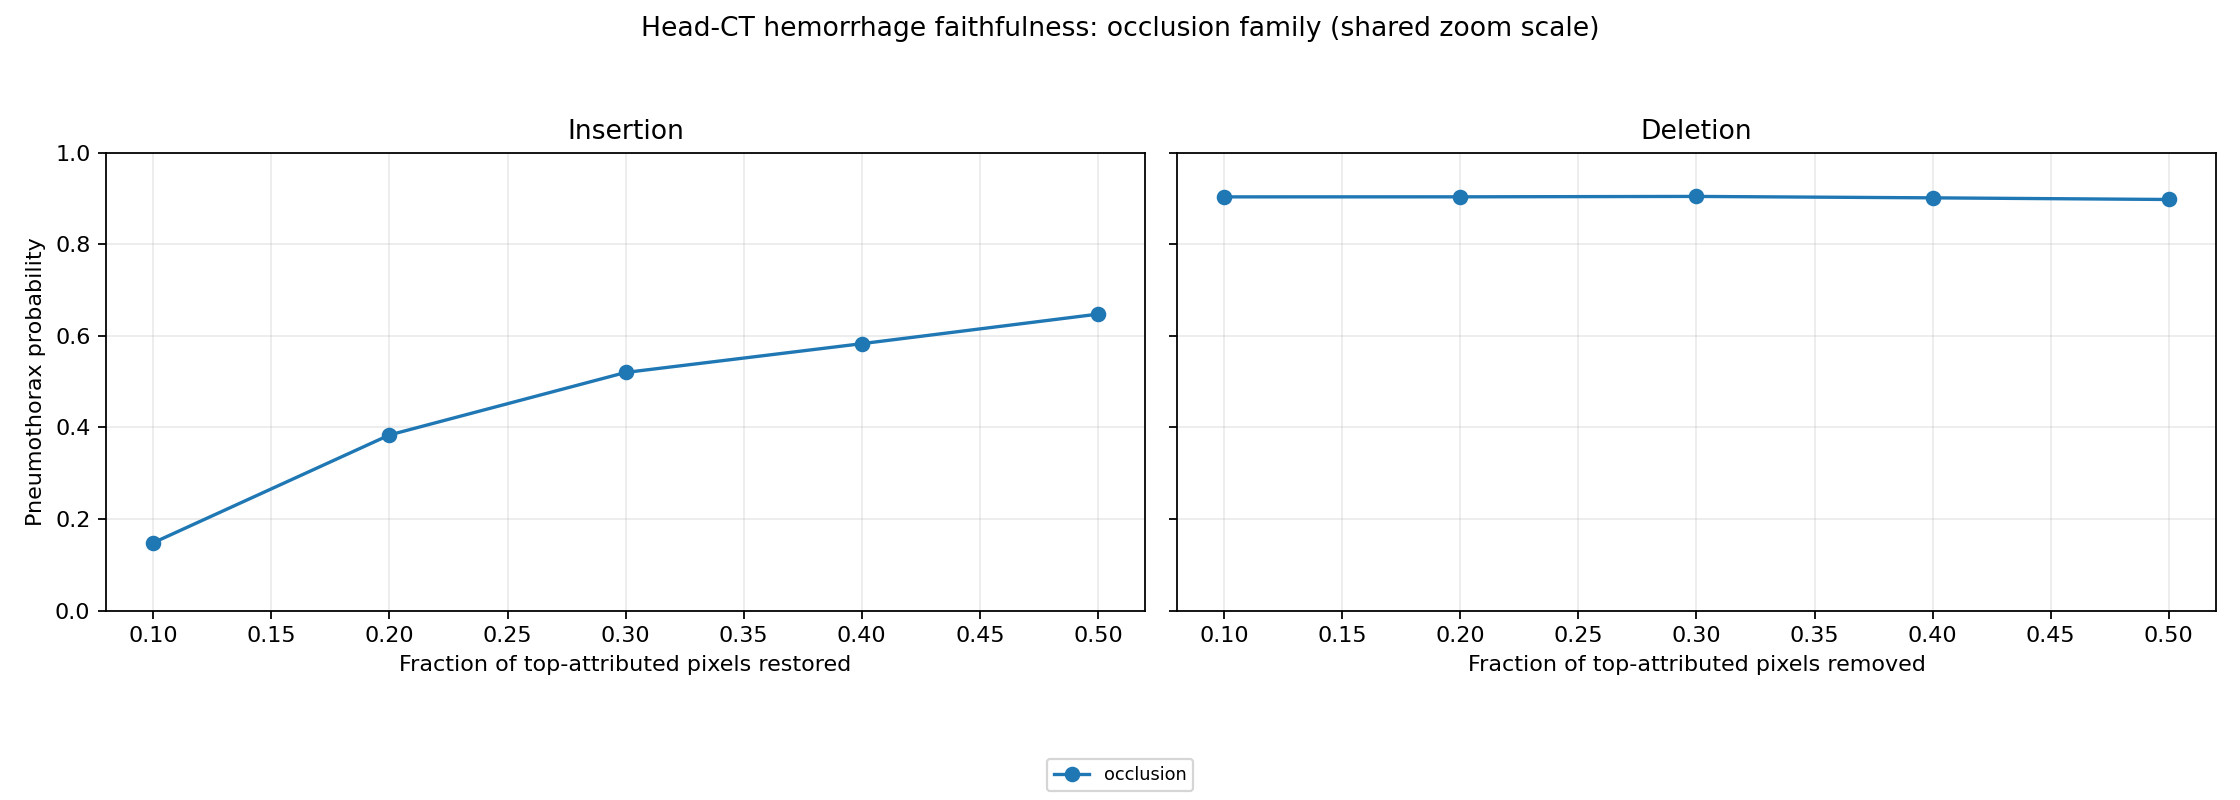
\includegraphics[width=0.85\linewidth,height=0.30\textheight,keepaspectratio]{figures/iter_53_ct_smoke_test__faithfulness_curves_occlusion_family.png}
		\subcaption{Occlusion family}
	\end{minipage}
	\caption{Faithfulness deletion and insertion curves for the CT model}
	\label{figure:c-4}
\end{figure}

Figure~\ref{figure:c-5} gives the consensus-versus-individual
localization box plots for the CT hemorrhage model.

\begin{figure}[htbp]
	\centering
	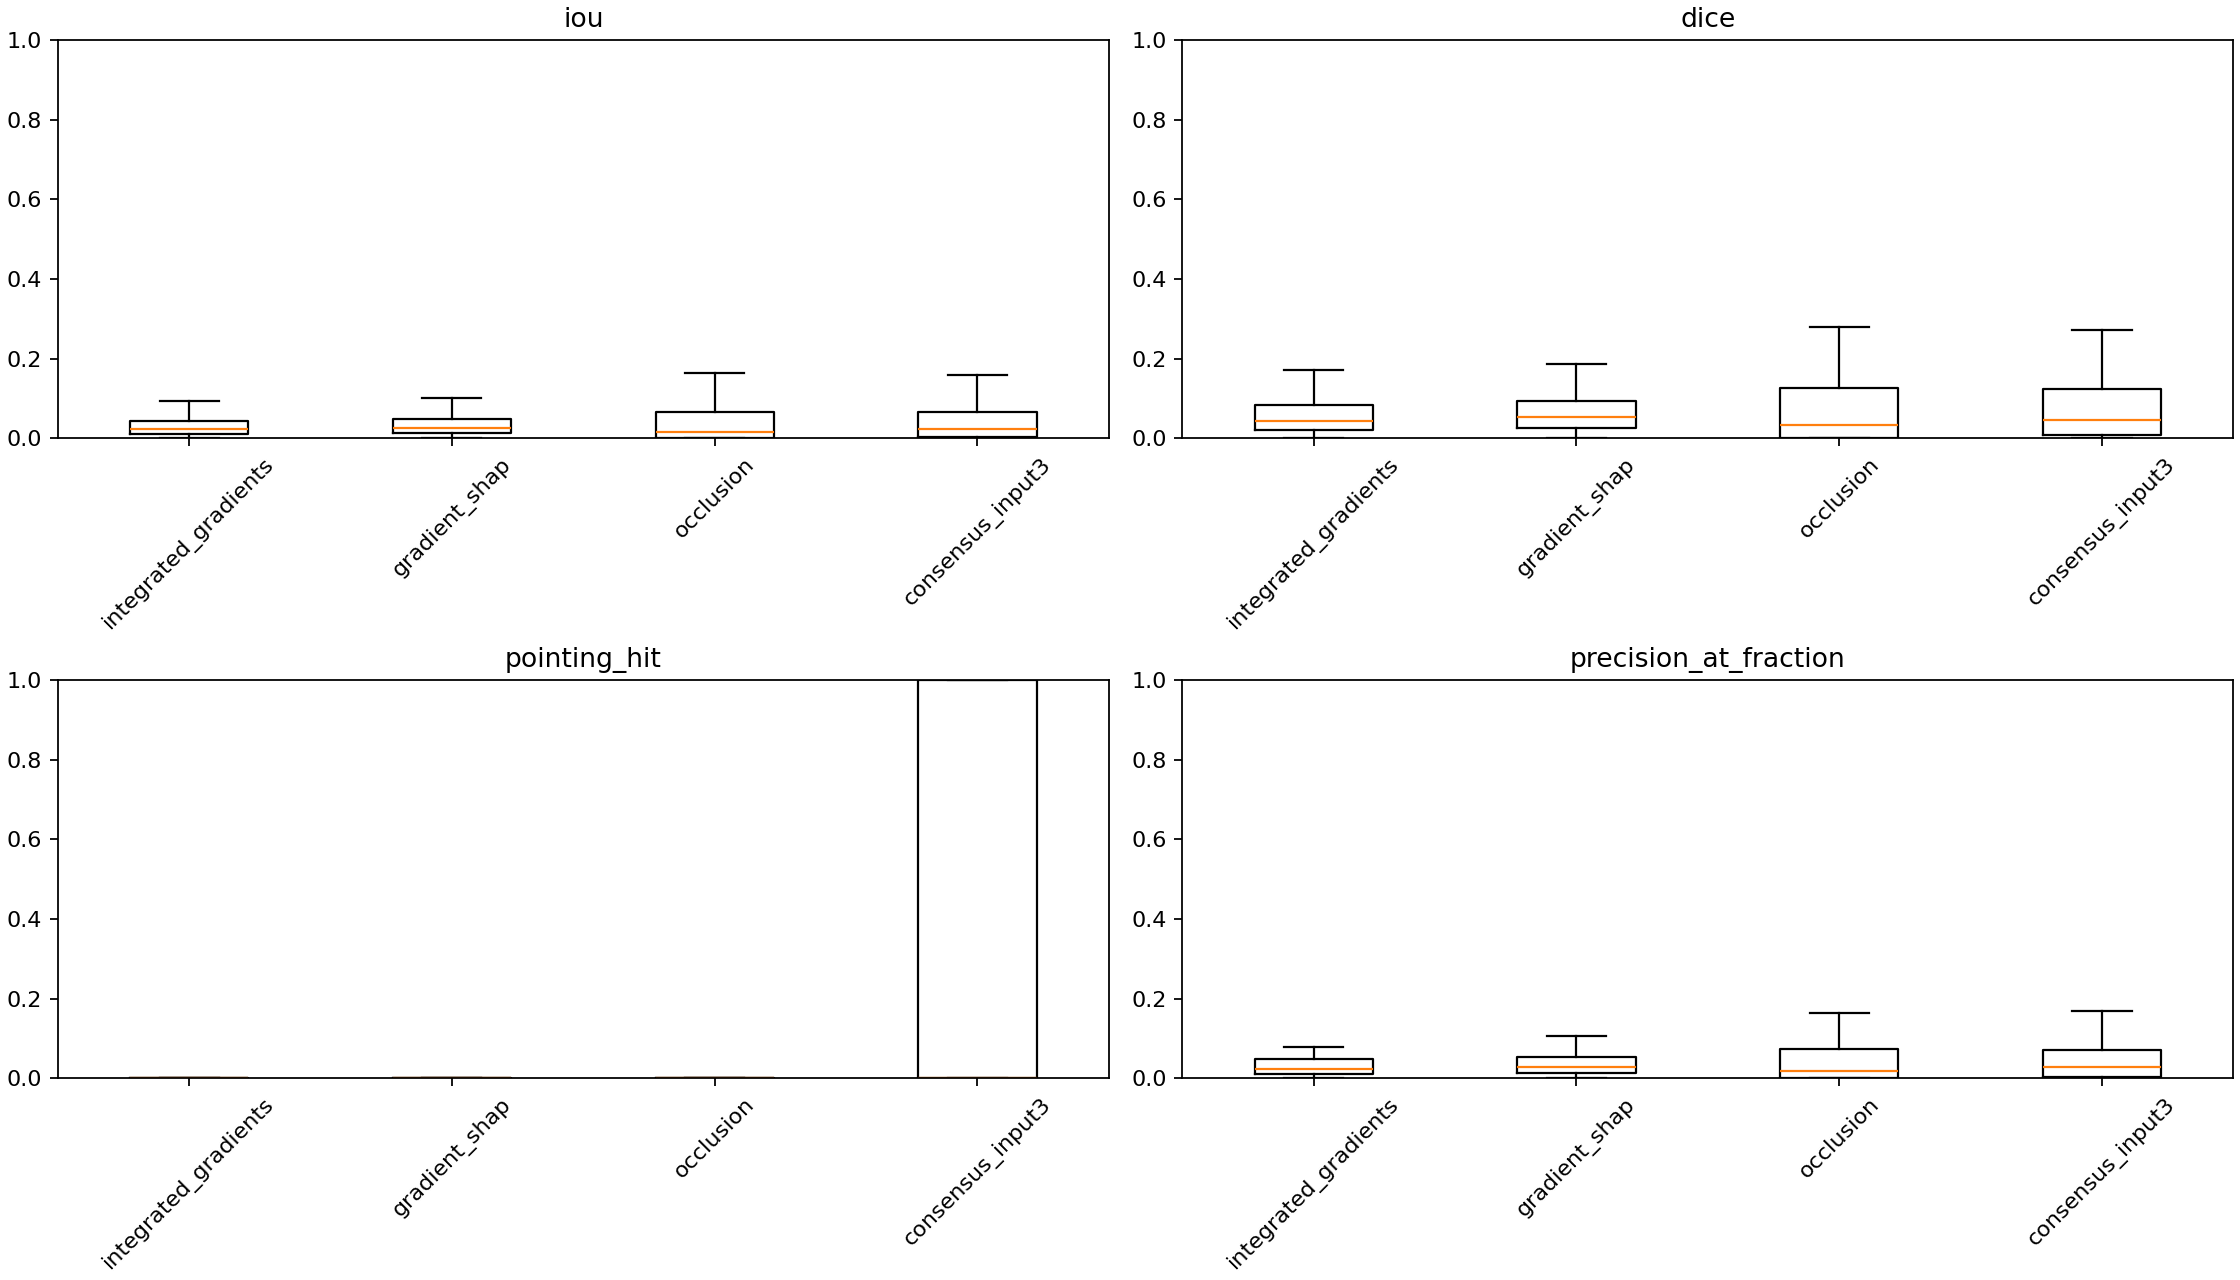
\includegraphics[width=0.85\linewidth,height=0.34\textheight,keepaspectratio]{figures/iter_54_ct_improvement_test__ct_improvement_experiment_boxplots.png}
	\caption{Consensus-versus-individual localization box plots for the CT model}
	\label{figure:c-5}
\end{figure}


% ===========================================================================
% Back matter (inserted after the body, before \end{document}, via pandoc -A).
% IEEE-style numbered bibliography harvested from docs/references.md.
% Note: in-text \cite wiring is intentionally left to the human pass; this is
% the formatted, numbered source list required by the template.
% ===========================================================================
\begin{thebibliography}{99}
\addcontentsline{toc}{chapter}{Bibliography}
\bibitem{ref1} R. R. Selvaraju, M. Cogswell, A. Das, R. Vedantam, D. Parikh, and D. Batra, "Grad-CAM: Visual Explanations From Deep Networks via Gradient-Based Localization," in \emph{Proceedings of the IEEE International Conference on Computer Vision (ICCV)}, 2017.

\bibitem{ref2} A. Chattopadhay, A. Sarkar, P. Howlader, and V. N. Balasubramanian, "Grad-CAM++: Generalized Gradient-Based Visual Explanations for Deep Convolutional Networks," in \emph{2018 IEEE Winter Conference on Applications of Computer Vision (WACV)}, 2018, pp. 839-847.

\bibitem{ref3} M. Sundararajan, A. Taly, and Q. Yan, "Axiomatic Attribution for Deep Networks," in \emph{Proceedings of the 34th International Conference on Machine Learning (ICML)}, PMLR, vol. 70, 2017, pp. 3319-3328.

\bibitem{ref4} S. M. Lundberg and S.-I. Lee, "A Unified Approach to Interpreting Model Predictions," in \emph{Advances in Neural Information Processing Systems}, 2017.

\bibitem{ref5} H. Wang, Z. Wang, M. Du, F. Yang, Z. Zhang, S. Ding, P. Mardziel, and X. Hu, "Score-CAM: Score-Weighted Visual Explanations for Convolutional Neural Networks," in \emph{2020 IEEE/CVF Conference on Computer Vision and Pattern Recognition Workshops (CVPRW)}, 2020, pp. 111-119.

\bibitem{ref6} M. D. Zeiler and R. Fergus, "Visualizing and Understanding Convolutional Networks," in \emph{Computer Vision -- ECCV 2014}, Lecture Notes in Computer Science, vol. 8689, Springer, 2014, pp. 818-833.

\bibitem{ref7} M. B. Muhammad and M. Yeasin, "Eigen-CAM: Class Activation Map using Principal Components," in \emph{2020 International Joint Conference on Neural Networks (IJCNN)}, 2020, pp. 1-7.

\bibitem{ref8} M. T. Ribeiro, S. Singh, and C. Guestrin, "'Why Should I Trust You?': Explaining the Predictions of Any Classifier," in \emph{Proceedings of the 22nd ACM SIGKDD International Conference on Knowledge Discovery and Data Mining (KDD)}, 2016, pp. 1135-1144.

\bibitem{ref9} Meta PyTorch, "Captum: Model Interpretability for PyTorch," official documentation and API reference.

\bibitem{ref10} J. Adebayo, J. Gilmer, M. Muelly, I. Goodfellow, M. Hardt, and B. Kim, "Sanity Checks for Saliency Maps," in \emph{Advances in Neural Information Processing Systems}, 2018.

\bibitem{ref11} C.-K. Yeh, C.-Y. Hsieh, A. S. Suggala, D. I. Inouye, and P. Ravikumar, "On the (In)fidelity and Sensitivity of Explanations," in \emph{Advances in Neural Information Processing Systems}, vol. 32, 2019.

\bibitem{ref12} V. Petsiuk, A. Das, and K. Saenko, "RISE: Randomized Input Sampling for Explanation of Black-box Models," in \emph{British Machine Vision Conference (BMVC)}, 2018.

\bibitem{ref13} W. Samek, A. Binder, G. Montavon, S. Lapuschkin, and K.-R. Muller, "Evaluating the Visualization of What a Deep Neural Network Has Learned," \emph{IEEE Transactions on Neural Networks and Learning Systems}, vol. 28, no. 11, pp. 2660-2673, 2017.

\bibitem{ref14} R. C. Fong and A. Vedaldi, "Interpretable Explanations of Black Boxes by Meaningful Perturbation," in \emph{Proceedings of the IEEE International Conference on Computer Vision (ICCV)}, 2017, pp. 3449-3457.

\bibitem{ref15} A. S. Ross, M. C. Hughes, and F. Doshi-Velez, "Right for the Right Reasons: Training Differentiable Models by Constraining their Explanations," in \emph{Proceedings of the Twenty-Sixth International Joint Conference on Artificial Intelligence (IJCAI-17)}, 2017, pp. 2662-2670.

\bibitem{ref16} N. Arun et al., "Assessing the Trustworthiness of Saliency Maps for Localizing Abnormalities in Medical Imaging," \emph{Radiology: Artificial Intelligence}, vol. 3, no. 6, Art. no. e200267, 2021.

\bibitem{ref17} A. Saporta et al., "Benchmarking saliency methods for chest X-ray interpretation," \emph{Nature Machine Intelligence}, vol. 4, pp. 867-878, 2022.

\bibitem{ref18} Stanford Center for Artificial Intelligence in Medicine and Imaging, "CheXlocalize," official dataset page; associated with A. Saporta et al., "Benchmarking saliency methods for chest X-ray interpretation," \emph{Nature Machine Intelligence}, 2022.

\bibitem{ref19} B. H. M. van der Velden, H. J. Kuijf, K. G. A. Gilhuijs, and M. A. Viergever, "Explainable artificial intelligence (XAI) in deep learning-based medical image analysis," \emph{Medical Image Analysis}, vol. 79, 2022, Art. no. 102470.

\bibitem{ref20} H. Chen, C. Gomez, C.-M. Huang, and M. Unberath, "Explainable medical imaging AI needs human-centered design: guidelines and evidence from a systematic review," \emph{npj Digital Medicine}, vol. 5, 2022, Art. no. 156.

\bibitem{ref21} A. DeGrave, J. D. Janizek, and S.-I. Lee, "AI for radiographic COVID-19 detection selects shortcuts over signal," \emph{Nature Machine Intelligence}, vol. 3, pp. 610-619, 2021.

\bibitem{ref22} J. R. Zech, M. A. Badgeley, M. Liu, A. B. Costa, J. J. Titano, and E. K. Oermann, "Variable generalization performance of a deep learning model to detect pneumonia in chest radiographs: A cross-sectional study," \emph{PLOS Medicine}, vol. 15, no. 11, Art. no. e1002683, 2018.

\bibitem{ref23} L. Oakden-Rayner, J. Dunnmon, G. Carneiro, and C. Re, "Hidden stratification causes clinically meaningful failures in machine learning for medical imaging," in \emph{Proceedings of the ACM Conference on Health, Inference, and Learning (CHIL)}, 2020, pp. 151-159.

\bibitem{ref24} M. Reyes, R. Meier, S. Pereira, C. A. Silva, F.-M. Dahlweid, H. von Tengg-Kobligk, R. M. Summers, and R. Wiest, "On the interpretability of artificial intelligence in radiology: challenges and opportunities," \emph{Radiology: Artificial Intelligence}, vol. 2, no. 3, Art. no. e190043, 2020.

\bibitem{ref25} M. Ghassemi, L. Oakden-Rayner, and A. L. Beam, "The false hope of current approaches to explainable artificial intelligence in health care," \emph{The Lancet Digital Health}, vol. 3, no. 11, pp. e745-e750, 2021.

\bibitem{ref26} R. Geirhos, J.-H. Jacobsen, C. Michaelis, R. Zemel, W. Brendel, M. Bethge, and F. A. Wichmann, "Shortcut learning in deep neural networks," \emph{Nature Machine Intelligence}, vol. 2, pp. 665-673, 2020.

\bibitem{ref27} I. Banerjee et al., "'Shortcuts' Causing Bias in Radiology Artificial Intelligence: Causes, Evaluation, and Mitigation," \emph{Journal of the American College of Radiology}, vol. 20, no. 9, pp. 842-851, 2023.

\bibitem{ref28} J. W. Gichoya et al., "AI recognition of patient race in medical imaging: a modelling study," \emph{The Lancet Digital Health}, vol. 4, no. 6, pp. e406-e414, 2022.

\bibitem{ref29} J. Mongan, L. Moy, and C. E. Kahn Jr., "Checklist for Artificial Intelligence in Medical Imaging (CLAIM): A Guide for Authors and Reviewers," \emph{Radiology: Artificial Intelligence}, vol. 2, no. 2, Art. no. e200029, 2020.

\bibitem{ref30} G. S. Collins et al., "TRIPOD+AI statement: updated guidance for reporting clinical prediction models that use regression or machine learning methods," \emph{BMJ}, vol. 385, Art. no. e078378, 2024.

\bibitem{ref31} V. Sounderajah et al., "A quality assessment tool for artificial intelligence-centered diagnostic test accuracy studies: QUADAS-AI," \emph{Nature Medicine}, vol. 27, no. 10, pp. 1663-1665, 2021.

\bibitem{ref32} B. Vasey et al. and the DECIDE-AI expert group, "Reporting guideline for the early-stage clinical evaluation of decision support systems driven by artificial intelligence: DECIDE-AI," \emph{Nature Medicine}, vol. 28, no. 5, pp. 924-933, 2022.

\bibitem{ref33} Society for Imaging Informatics in Medicine (SIIM), "SIIM-ACR Pneumothorax Segmentation Kaggle Challenge," official challenge information page.

\bibitem{ref34} J. P. Cohen et al., "TorchXRayVision: A library of chest X-ray datasets and models," in \emph{Proceedings of the 5th International Conference on Medical Imaging with Deep Learning}, PMLR, vol. 172, 2022, pp. 231-249.

\bibitem{ref35} X. Wang, Y. Peng, L. Lu, Z. Lu, M. Bagheri, and R. M. Summers, "ChestX-Ray8: Hospital-Scale Chest X-Ray Database and Benchmarks on Weakly-Supervised Classification and Localization of Common Thorax Diseases," in \emph{Proceedings of the IEEE Conference on Computer Vision and Pattern Recognition (CVPR)}, 2017, pp. 3462-3471.

\bibitem{ref36} P. Rajpurkar et al., "Deep learning for chest radiograph diagnosis: A retrospective comparison of the CheXNeXt algorithm to practicing radiologists," \emph{PLOS Medicine}, vol. 15, no. 11, Art. no. e1002686, 2018.

\bibitem{ref37} J. Irvin et al., "CheXpert: A Large Chest Radiograph Dataset with Uncertainty Labels and Expert Comparison," in \emph{Proceedings of the AAAI Conference on Artificial Intelligence}, vol. 33, no. 1, 2019, pp. 590-597.

\bibitem{ref38} A. E. W. Johnson et al., "MIMIC-CXR, a de-identified publicly available database of chest radiographs with free-text reports," \emph{Scientific Data}, vol. 6, Art. no. 317, 2019.

\bibitem{ref39} H. Q. Nguyen et al., "VinDr-CXR: An open dataset of chest X-rays with radiologist's annotations," \emph{Scientific Data}, vol. 9, Art. no. 429, 2022.

\bibitem{ref40} F. Wilcoxon, "Individual Comparisons by Ranking Methods," \emph{Biometrics Bulletin}, vol. 1, no. 6, pp. 80-83, 1945.

\bibitem{ref41} S. Holm, "A Simple Sequentially Rejective Multiple Test Procedure," \emph{Scandinavian Journal of Statistics}, vol. 6, no. 2, pp. 65-70, 1979.

\bibitem{ref42} M. Aickin and H. Gensler, "Adjusting for Multiple Testing When Reporting Research Results: The Bonferroni vs Holm Methods," \emph{American Journal of Public Health}, vol. 86, no. 5, pp. 726-728, 1996.

\bibitem{ref43} J. Demšar, "Statistical Comparisons of Classifiers over Multiple Data Sets," \emph{Journal of Machine Learning Research}, vol. 7, pp. 1-30, 2006.

\bibitem{ref44} A. E. Flanders et al., "Construction of a Machine Learning Dataset through Collaboration: The RSNA 2019 Brain CT Hemorrhage Challenge," \emph{Radiology: Artificial Intelligence}, vol. 2, no. 3, Art. no. e190211, 2020.

\bibitem{ref45} A. Dosovitskiy, L. Beyer, A. Kolesnikov, D. Weissenborn, X. Zhai, T. Unterthiner, M. Dehghani, M. Minderer, G. Heigold, S. Gelly, J. Uszkoreit, and N. Houlsby, "An Image Is Worth 16x16 Words: Transformers for Image Recognition at Scale," in \emph{Proc. International Conference on Learning Representations (ICLR)}, 2021.

\bibitem{ref46} S. Abnar and W. Zuidema, "Quantifying Attention Flow in Transformers," in \emph{Proc. 58th Annual Meeting of the Association for Computational Linguistics (ACL)}, 2020, pp. 4190-4197.

\bibitem{ref47} H. Chefer, S. Gur, and L. Wolf, "Transformer Interpretability Beyond Attention Visualization," in \emph{Proc. IEEE/CVF Conference on Computer Vision and Pattern Recognition (CVPR)}, 2021, pp. 782-791.

\bibitem{ref48} W. Xie, X.-H. Li, C. C. Cao, and N. L. Zhang, "ViT-CX: Causal Explanation of Vision Transformers," in \emph{Proc. 32nd International Joint Conference on Artificial Intelligence (IJCAI)}, 2023.

\bibitem{ref49} J. Gildenblat and contributors, \emph{PyTorch library for CAM methods (pytorch-grad-cam)}, GitHub repository, 2021.
\end{thebibliography}


\end{document}
